\chapter{Sequenti\"ele Schakelingen (Schakelingen met geheugen)}
\label{ch:SeqComp}
\chapterquote{We denken dat sommige mensen intelligent zijn, terwijl ze alleen maar een goed geheugen hebben.}{Fr\'ed\'eric Dard, Frans humoristisch schrijver (1921-2000)}
\begin{chapterintro}
??
\end{chapterintro}
\minitoc[n]
\section{Terminologie}
Een \termen{Sequenti\"ele schakeling} is een schakeling waarbij niet alleen de ingangen $X$ van belang zijn, maar ook de toestand van deze schakeling. De \termen{toestand $S$} wordt bepaald door de ingang, en door de vorige toestand $S_{\mbox{\tiny{prev.}}}$. In de wiskunde wordt een dergelijke constructie beschreven als een \termen{eindige-toestanden machine} of \termen{finite state machine (FSM)}. Om dit te verwezenlijken hebben we een \termen{geheugencomponent} nodig, een component die de toestand bijhoudt. Dit kunnen we bijvoorbeeld verwezenlijken met een condensator. In DRAM geheugens wordt dergelijke implementatie gebruikt. Het probleem met een condensator is dat de lading na verloop van tijd verloren gaat, wat tot dynamische logica leidt. In DRAM wordt dit opgelost door de condensatoren in kwestie terug op te laden. Een alternatief zijn componenten met \termen{positieve terugkoppeling}, doorgaans zijn deze bekend als \termen{flipflop} of \termen{register}. In sectie \ref{s:memoryBlocks} zullen we verschillende van deze bouwblokken bespreken.
\subsection{Classificatie van sequenti\"ele schakelingen}
\label{ss:classificationSequential}
Doorgaans kunnen we sequenti\"ele schakelingen onderverdelen volgens twee classificatiesystemen: gebaseerd op de uitgangsfunctie $F$, en de synchroniciteit van de schakeling. Wat betreft de uitgangsfunctie beschouwen we twee types:
\begin{itemize}
 \item \termen{Toestandsgebonden sequenti\"ele schakelingen}: In dit geval hangt de uitgangsfunctie enkel af van de toestand op dat moment. In dat geval is de uitgangsfunctie $F\left(S\right)$. Dit concept is ook bekend als de \termen{Moore machine} ofwel \termen{Moore-FSM}. Bij een Moore machine is de invloed van de ingang dus met vertraging te zien, vermits de schakeling eerste van toestand moet veranderen.
 \item \termen{Inputgebonden sequenti\"ele schakelingen}: Hierbij wordt de signatuur van de uitgangsfunctie uitgebreid. De uitgang is zowel afhankelijk van de toestand $S$ als van de ingang $X$. Dit betekent dat indien de ingang verandert, maar de toestand niet de uitvoer $F\left(S,X\right)$ ook verandert. Dit concept wordt ook wel de \termen{Mealy machine} ofwel \termen{Mealy-FSM} genoemd. Elke Moore machine is dus ook een Mealy machine waar de invoer geen onderdeel uitmaakt van de logica die de uitgang berekend.
\end{itemize}
Verder maken we ook een onderscheid in schakelingen inzake synchroniciteit, ook hier beschouwen we twee soorten:
\begin{itemize}
 \item \termen{Asynchrone sequenti\"ele schakelingen}: Hierbij verandert uitgang $F$ en toestand $S$ wanneer de ingang $X$ verandert. We zullen asynchrone schakelingen kort in sectie \ref{s:asynchroneSequence}, bovendien zullen we veronderstellen dat slechts \'e\'en bit tegelijk verandert aan de ingang.
 \item \termen{Synchrone sequenti\"ele schakelingen}: Hierbij veranderen de uitgang $F$ en toestand $S$ enkel op het moment de zogenoemde \termen{klokingang} verandert.
Veruit de meeste sequenti\"ele schakelingen worden gebouwd op basis van een klok. In sectie \ref{s:synchroneSequence} zullen we uitgebreid synchrone schakelingen en hun synthese bespreken.
\end{itemize}
\subsection{Terminologie van het kloksignaal}
Bij synchrone schakelingen maken we gebruik van een klokingang. Op deze klokingang staat periodiek een 0 gevolgd door een 1. Om dit kloksignaal te beschrijven maken we gebruik van de volgende terminologie:
\begin{itemize}
 \item \termen{Klokperiode}: de tijd tussen twee opeenvolgende klokovergangen van 0 naar 1.
 \item \termen{Klokfrequentie}: het aantal klokperiodes per seconden of formeler:
\begin{equation}
\mbox{klokfrequentie}=\displaystyle\frac{1}{\mbox{klokperiode}}
\end{equation}
 \item ``\termen{Duty cycle}'': fragment van de klokcyclus die dat de klok op 1 staat.
\begin{equation}
\mbox{duty cycle}=\displaystyle\frac{\mbox{tijd klok is 1}}{\mbox{klokperiode}}
\end{equation}
De klok staat dus niet per definitie even lang op 0 als op 1.
 \item \termen{Stijgende flank} (ook wel \termen{rising edge} genoemd): de klokovergang waarbij de klok van 0 naar 1 gaat.
 \item \termen{Dalende flank} (ook wel \termen{falling edge} genoemd): de klokovergang waarbij de klok van 1 naar 0 gaat.
\end{itemize}
\section{Bouwblokken}
\label{s:memoryBlocks}
In deze sectie zullen we de bouwblokken van geheugen ontwikkelen. Hierbij zullen we in subsectie \ref{ss:flipflop} eerst het basisblok ontwikkelen om \'e\'en bit te onthouden: de flipflop. Door flipflops te groeperen kunnen we een groter geheugen ontwikkelen. Dergelijke geheugens worden registers genoemd. Registers kunnen meestal maar een beperkt aantal flipflops tegelijk aanspreken. Registers bespreken we in subsectie \ref{ss:registers}. Een andere populaire toepassing van geheugens is een teller. We ontwikkelen een tellerschakeling in subsectie \ref{ss:counters}.
\subsection{De flipflop}
\label{ss:flipflop}
Bij de synthese van een flipflop zullen we een eerste positief feedback component introduceren: de \termen{set-reset latch}. Vervolgens zullen we deze latch uitbreiden en verschillende varianten bespreken. Een probleem met latches is het zogenaamde \termen{transparantie-probleem}. Dit probleem zullen we oplossen door extra logica met deze latch te verbinden wat resulteert in een \termen{flipflop}. Er zijn verschillende varianten van flipflops om verschillende toepassingen te ondersteunen, we eindigen met een beknopt overzicht van de verschillende flipflops.
\subsubsection{De latch}
\begin{figure}[hbt]
\centering
\subfigure[Implementatie met NOR-poorten.]{\begin{tikzpicture}[circuit logic US]
\node[nor gate] (NO0) at (0,0.65) {};
\node[nor gate] (NO1) at (0,-0.65) {};
\draw (NO0.input 1) -- (NO0.input 1 -| -1,0) node[anchor=east,scale=0.75]{Set $S$};
\draw (NO1.input 2) -- (NO1.input 2 -| -1,0) node[anchor=east,scale=0.75]{Reset $R$};
\draw (NO0.output) -- (NO0.output -| 1.1,0) node[anchor=west,scale=0.75]{$Q_n$};
\draw (NO1.output) -- (NO1.output -| 1.1,0) node[anchor=west,scale=0.75]{$Q$};
\pdot{NO0.output -| 0.85,0};
\pdot{NO1.output -| 0.85,0};
\draw (NO1.output -| 0.85,0) -- (0.85,-0.4) -- (-0.75,0.4) -- (NO0.input 2 -| -0.75,0) -- (NO0.input 2);
\draw (NO0.output -| 0.85,0) -- (0.85,0.4) -- (-0.75,-0.4) -- (NO1.input 1 -| -0.75,0) -- (NO1.input 1);
\node[scale=0.75] (TT) at (3,0) {$\begin{array}{cc|c}S&R&Q_{\mbox{\tiny{next}}}\\\hline0&0&Q\\0&1&0\\1&0&1\\1&1&\mbox{N/A}\end{array}$};
%\timebehav{5}{-1}{8.5}{4}{0.75}{0/$Q_n$,1/$Q$,2/$R$,3/$S$}{3/0/0/1/1,3/1/1/2/0,3/2/0/5/1,3/5/1/7/0,3/7/0/9/1,3/9/1/10/0,3/10/0/11.5/0, 2/0/0/3/1,2/3/1/4/0,2/4/0/6/1,2/6/1/8/0,2/8/0/9/1,2/9/1/10/0,2/10/0/11.5/0, 1/0/0/1.5/1,1/1.5/1/3.25/0,1/3.25/0/5.5/1,1/5.5/1/6.25/0,1/6.25/0/10.25/1,1/10.25/1/10.5/0,1/10.5/0/10.75/1,1/10.75/1/11/0,1/11/0/11.25/1,1/11.25/1/11.5/1, 0/0/1/1.25/0,0/1.25/0/3.5/1,0/3.5/1/5.25/0,0/5.25/0/7.25/1,0/7.25/1/9.25/0,0/9.25/0/10.25/1,0/10.25/1/10.5/0,0/10.5/0/10.75/1,0/10.75/1/11/0,0/11/0/11.25/1,0/11.25/1/11.5/1}{1/0.25/3/0,1.25/0.25/0/1,3/0.25/2/1,3.25/0.25/1/0,5/0.25/3/0,5.25/0.25/0/1,6/0.25/2/1,7/0.25/3/0,9/0.25/3/0,10/0.25/3/0,10/0.25/2/1,10.25/0.25/1/0,10.25/0.25/0/1,10.5/0.25/1/0,10.5/0.25/0/1,10.75/0.25/1/0,10.75/0.25/0/1,11/0.25/1/0,11/0.25/0/1};
\timebehav{5.00}{-1.00}{8.50}{4}{0.75}{0/$Q_n$,1/$Q$,2/$R$,3/$S$}{0/0.00/1/1.25/0, 0/1.25/0/3.50/1, 0/3.50/1/5.25/0, 0/5.25/0/7.25/1, 0/7.25/1/9.25/0, 0/9.25/0/10.25/1, 0/10.25/1/10.50/0, 0/10.50/0/10.75/1, 0/10.75/1/11.00/0, 0/11.00/0/11.25/1, 0/11.25/1/11.48/1, 1/0.00/0/1.50/1, 1/1.50/1/3.25/0, 1/3.25/0/5.50/1, 1/5.50/1/6.25/0, 1/6.25/0/10.25/1, 1/10.25/1/10.50/0, 1/10.50/0/10.75/1, 1/10.75/1/11.00/0, 1/11.00/0/11.25/1, 1/11.25/1/11.48/1, 2/0.00/0/3.00/1, 2/3.00/1/4.00/0, 2/4.00/0/6.00/1, 2/6.00/1/8.00/0, 2/8.00/0/9.00/1, 2/9.00/1/10.00/0, 2/10.00/0/11.48/0, 3/0.00/0/1.00/1, 3/1.00/1/2.00/0, 3/2.00/0/5.00/1, 3/5.00/1/7.00/0, 3/7.00/0/9.00/1, 3/9.00/1/10.00/0, 3/10.00/0/11.48/0}{1.00/0.25/3/0, 3.25/0.25/1/0, 5.00/0.25/3/0, 7.00/0.25/3/0, 9.00/0.25/3/0, 10.00/0.25/3/0, 10.25/0.25/1/0, 10.50/0.25/1/0, 10.75/0.25/1/0, 11.00/0.25/1/0, 1.25/0.25/0/1, 3.00/0.25/2/1, 5.25/0.25/0/1, 6.00/0.25/2/1, 10.00/0.25/2/1, 10.25/0.25/0/1, 10.50/0.25/0/1, 10.75/0.25/0/1, 11.00/0.25/0/1};
\end{tikzpicture}}
\subfigure[Implementatie met NAND-poorten.]{\begin{tikzpicture}[circuit logic US]
\node[nand gate] (NO0) at (0,0.65) {};
\node[nand gate] (NO1) at (0,-0.65) {};
\draw (NO0.input 1) -- (NO0.input 1 -| -1,0) node[anchor=east,scale=0.75]{Set $S^*$};
\draw (NO1.input 2) -- (NO1.input 2 -| -1,0) node[anchor=east,scale=0.75]{Reset $R^*$};
\draw (NO0.output) -- (NO0.output -| 1.1,0) node[anchor=west,scale=0.75]{$Q$};
\draw (NO1.output) -- (NO1.output -| 1.1,0) node[anchor=west,scale=0.75]{$Q_n$};
\pdot{NO0.output -| 0.85,0};
\pdot{NO1.output -| 0.85,0};
\draw (NO1.output -| 0.85,0) -- (0.85,-0.4) -- (-0.75,0.4) -- (NO0.input 2 -| -0.75,0) -- (NO0.input 2);
\draw (NO0.output -| 0.85,0) -- (0.85,0.4) -- (-0.75,-0.4) -- (NO1.input 1 -| -0.75,0) -- (NO1.input 1);
\node[scale=0.75] (TT) at (3,0) {$\begin{array}{cc|c}S^*&R^*&Q_{\mbox{\tiny{next}}}\\\hline1&1&Q\\1&0&0\\0&1&1\\0&0&\mbox{N/A}\end{array}$};
%\timebehav{5}{-1}{8.5}{4}{0.75}{0/$Q_n$,1/$Q$,2/$R^*$,3/$S^*$}{3/0/1/1/0,3/1/0/2/1,3/2/1/5/0,3/5/0/7/1,3/7/1/9/0,3/9/0/10/1,3/10/1/11.5/1, 2/0/1/3/0,2/3/0/4/1,2/4/1/6/0,2/6/0/8/1,2/8/1/9/0,2/9/0/10/1,2/10/1/11.5/1, 1/0/0/1.5/1,1/1.5/1/3.25/0,1/3.25/0/5.5/1,1/5.5/1/6.25/0,1/6.25/0/10.25/1,1/10.25/1/10.5/0,1/10.5/0/10.75/1,1/10.75/1/11/0,1/11/0/11.25/1,1/11.25/1/11.5/1, 0/0/1/1.25/0,0/1.25/0/3.5/1,0/3.5/1/5.25/0,0/5.25/0/7.25/1,0/7.25/1/9.25/0,0/9.25/0/10.25/1,0/10.25/1/10.5/0,0/10.5/0/10.75/1,0/10.75/1/11/0,0/11/0/11.25/1,0/11.25/1/11.5/1}{1/0.25/3/0,1.25/0.25/0/1,3/0.25/2/1,3.25/0.25/1/0,5/0.25/3/0,5.25/0.25/0/1,6/0.25/2/1,7/0.25/3/0,9/0.25/3/0,10/0.25/3/0,10/0.25/2/1,10.25/0.25/1/0,10.25/0.25/0/1,10.5/0.25/1/0,10.5/0.25/0/1,10.75/0.25/1/0,10.75/0.25/0/1,11/0.25/1/0,11/0.25/0/1};
\timebehav{5.00}{-1.00}{8.50}{4}{0.75}{0/$Q_n$,1/$Q$,2/$R^*$,3/$S^*$}{0/0.00/1/1.50/0, 0/1.50/0/3.25/1, 0/3.25/1/5.50/0, 0/5.50/0/6.25/1, 0/6.25/1/10.25/0, 0/10.25/0/10.50/1, 0/10.50/1/10.75/0, 0/10.75/0/11.00/1, 0/11.00/1/11.25/0, 0/11.25/0/11.48/0, 1/0.00/0/1.25/1, 1/1.25/1/3.50/0, 1/3.50/0/5.25/1, 1/5.25/1/7.25/0, 1/7.25/0/9.25/1, 1/9.25/1/10.25/0, 1/10.25/0/10.50/1, 1/10.50/1/10.75/0, 1/10.75/0/11.00/1, 1/11.00/1/11.25/0, 1/11.25/0/11.48/0, 2/0.00/1/3.00/0, 2/3.00/0/4.00/1, 2/4.00/1/6.00/0, 2/6.00/0/8.00/1, 2/8.00/1/9.00/0, 2/9.00/0/10.00/1, 2/10.00/1/11.48/1, 3/0.00/1/1.00/0, 3/1.00/0/2.00/1, 3/2.00/1/5.00/0, 3/5.00/0/7.00/1, 3/7.00/1/9.00/0, 3/9.00/0/10.00/1, 3/10.00/1/11.48/1}{1.25/0.25/1/0, 3.00/0.25/2/0, 5.25/0.25/1/0, 6.00/0.25/2/0, 10.00/0.25/2/0, 10.25/0.25/1/0, 10.50/0.25/1/0, 10.75/0.25/1/0, 11.00/0.25/1/0, 1.00/0.25/3/1, 3.25/0.25/0/1, 5.00/0.25/3/1, 7.00/0.25/3/1, 9.00/0.25/3/1, 10.00/0.25/3/1, 10.25/0.25/0/1, 10.50/0.25/0/1, 10.75/0.25/0/1, 11.00/0.25/0/1};
\end{tikzpicture}}
\caption{Set-reset latch.}
\label{fig:setResetLatch}
\end{figure}
Figuur \ref{fig:setResetLatch} toont de NOR- en NAND-implementatie van de zogenaamde set-reset latch (ofwel \termen{SR-latch}). Dit component werkt met positieve terugkoppeling waarbij de uitgangen dus ook een deel van de ingangen vormen. We onthouden de uitvoer door bepaalde waarden aan de ingang aan te leggen, die resulteren in het opnieuw bekomen van dezelfde uitvoer. Bij de NOR-implementatie is dit $\left(S,R\right)=\left(0,0\right)$. De NAND-implementatie is in feite de volledig duale vorm en werkt volledig equivalent, alleen zijn $S$ en $R$ hier laag actieve signalen (zie \ref{s:negativeLogic}). We zouden ook negatieve logica aan $Q$ en $Q_n$ moeten toekennen maar omdat altijd geldt $Q_n=Q'$ kunnen we ook eenvoudigweg de twee uitgangen omdraaien en bekomen we positieve logica aan de uitgang. De stabiele invoer van de NAND-implementatie is dan ook $\left(S^*,R^*\right)=\left(1,1\right)$. Indien we \'e\'en van de ingangen laten afwijken van de stabiele toestand, komen we in een onstabiele toestand. Deze stabiele toestand kan maar op \'e\'en manier terug stabiel worden. Op deze manier kunnen we een nieuwe waarde toekennen aan de latch. Deze waarde zal ook verder gelden nadat de ingangen weer stabiel zijn. Hierdoor kent men ook de termen \termen{set} (1 in het geheugen) en \termen{reset} (0 in het geheugen) toe aan de ingangen. Indien beide ingangen afwijken van de stabiele ingangen is het gedrag niet meer bepaald. In dat geval zal de uiteindelijke waarde afhangen van de implementatie van de latch en de vertraging van de poorten. Bij identieke vertragingen leidt dit tot een oscillerend effect wat ook te zien is op de tijdsgrafieken op figuur \ref{fig:setResetLatch}. In een minder ideaal systeem zal de snelste poort\footnote{Uiteraard zijn de twee poorten in theorie even traag, in de praktijk zullen er altijd kleine verschillen zijn.} de uiteindelijke vertraging bepalen. Dit gedrag noemt men een ``\termen{race}'' (zie \ref{term:race}).
\paragraph{Geklokte SR-latch}
Bij de SR-latch is er geen sprake van een klokingang. We kunnen immers ook geheugens zonder klok gebruiken in bijvoorbeeld asynchrone schakelingen. Door extra hardware voor de SR-latch te plaatsen, kunnen we een \termen{geklokte SR-latch} bouwen. Figuur \ref{fig:clockedSRLatch} toont hoe we dit kunnen realiseren. Zolang het kloksignaal op 0 staat zal het geheugen zijn waarde behouden, indien het kloksignaal op 1 staat gelden dezelfde regels als bij een SR-latch.
\begin{figure}[hbt]
\centering
\subfigure[Met AND- en NOR-poorten.]{\begin{tikzpicture}[circuit logic US]
\node[nor gate] (NO0) at (0,0.65) {};
\node[nor gate] (NO1) at (0,-0.65) {};
\node[and gate,anchor=output] (A0) at (NO0.input 1 -| -1,0) {};
\node[and gate,anchor=output] (A1) at (NO1.input 2 -| -1,0) {};
\draw (A0.output) -- (NO0.input 1);
\draw (A1.output) -- (NO1.input 2);
\draw (A0.input 2) -- (A0.input 2 -| -2,0) |- (A1.input 1);
\pdot{-2,0};
\draw (A0.input 1) -- (A0.input 1 -| -2.5,0) node[anchor=east,scale=0.75]{Set $S$};
\draw (-2,0) -- (-2.5,0) node[anchor=east,scale=0.75]{Klok Clk};
\draw (A1.input 2) -- (A1.input 2 -| -2.5,0) node[anchor=east,scale=0.75]{Reset $R$};
\draw (NO0.output) -- (NO0.output -| 1.1,0) node[anchor=west,scale=0.75]{$Q_n$};
\draw (NO1.output) -- (NO1.output -| 1.1,0) node[anchor=west,scale=0.75]{$Q$};
\pdot{NO0.output -| 0.85,0};
\pdot{NO1.output -| 0.85,0};
\draw (NO1.output -| 0.85,0) -- (0.85,-0.4) -- (-0.75,0.4) -- (NO0.input 2 -| -0.75,0) -- (NO0.input 2);
\draw (NO0.output -| 0.85,0) -- (0.85,0.4) -- (-0.75,-0.4) -- (NO1.input 1 -| -0.75,0) -- (NO1.input 1);
\end{tikzpicture}}
\subfigure[Met NAND-poorten.]{\begin{tikzpicture}[circuit logic US]
\node[nand gate] (NO0) at (0,0.65) {};
\node[nand gate] (NO1) at (0,-0.65) {};
\node[nand gate,anchor=output] (NA0) at (NO0.input 1 -| -1,0) {};
\node[nand gate,anchor=output] (NA1) at (NO1.input 2 -| -1,0) {};
\draw (NA0.output) -- (NO0.input 1);
\draw (NA1.output) -- (NO1.input 2);
\draw (NA0.input 2) -- (NA0.input 2 -| -2,0) |- (NA1.input 1);
\pdot{-2,0};
\draw (NA0.input 1) -- (NA0.input 1 -| -2.5,0) node[anchor=east,scale=0.75]{Set $S$};
\draw (-2,0) -- (-2.5,0) node[anchor=east,scale=0.75]{Klok Clk};
\draw (NA1.input 2) -- (NA1.input 2 -| -2.5,0) node[anchor=east,scale=0.75]{Reset $R$};
\draw (NO0.output) -- (NO0.output -| 1.1,0) node[anchor=west,scale=0.75]{$Q$};
\draw (NO1.output) -- (NO1.output -| 1.1,0) node[anchor=west,scale=0.75]{$Q_n$};
\pdot{NO0.output -| 0.85,0};
\pdot{NO1.output -| 0.85,0};
\draw (NO1.output -| 0.85,0) -- (0.85,-0.4) -- (-0.75,0.4) -- (NO0.input 2 -| -0.75,0) -- (NO0.input 2);
\draw (NO0.output -| 0.85,0) -- (0.85,0.4) -- (-0.75,-0.4) -- (NO1.input 1 -| -0.75,0) -- (NO1.input 1);
\end{tikzpicture}}
\subfigure[Overgangstabel]{
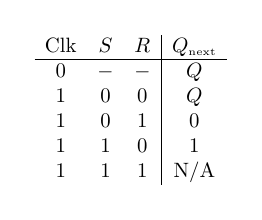
\begin{tikzpicture}
\node[scale=0.75] (TT) at (3,0) {$\begin{array}{ccc|c}\mbox{Clk}&S&R&Q_{\mbox{\tiny{next}}}\\\hline0&-&-&Q\\1&0&0&Q\\1&0&1&0\\1&1&0&1\\1&1&1&\mbox{N/A}\end{array}$};
\end{tikzpicture}
}
\caption{Geklokte SR-latch.}
\label{fig:clockedSRLatch}
\end{figure}
\paragraph{Geklokte D-latch}
Indien we elke klokflank een nieuwe waarde in de latch willen opslaan loont het meestal de moeite om de geklokte SR-latch om te vormen tot een \termen{geklokte D-latch}. Een geklokte D-latch zoals op figuur \ref{fig:clockedDLatch} bouwt meestal extra logica rond een geklokte SR-latch die met de \termen{data-ingang $D$} de $S$ en $R$ ingang aanstuurt. D-latches zijn populair bij schakelingen waarbij bij iedere klokflank een nieuwe waarde wordt ingelezen. Soms wordt dan echter ook een SR-latch gebruikt omdat dit de logica rond deze geheugenmodules soms kan vereenvoudigen.
\begin{figure}[hbt]
\centering
\subfigure[Implementatie.]{\begin{tikzpicture}[circuit logic US]
\node[nand gate] (NO0) at (0,0.65) {};
\node[nand gate] (NO1) at (0,-0.65) {};
\node[nand gate,anchor=output] (NA0) at (NO0.input 1 -| -1,0) {};
\node[nand gate,anchor=output] (NA1) at (NO1.input 2 -| -1,0) {};
\node[not gate,anchor=output,rotate=-90,scale=0.6] (N0) at (NA1.input 1 -| -2.25,0) {};
\draw (NA0.output) -- (NO0.input 1);
\draw (NA1.output) -- (NO1.input 2);
\draw (NA0.input 2) -- (NA0.input 2 -| -2,0) |- (NA1.input 1);
\pdot{-2,0};
\draw (NA0.input 1) -- (NA0.input 1 -| -2.5,0) node[anchor=east,scale=0.75]{Data $D$};
\draw (-2,0) -- (-2.5,0) node[anchor=east,scale=0.75]{Klok Clk};
\draw (NA1.input 2) -| (N0.output);
\draw (N0.input) -- (N0.input |- NA0.input 1);
\pdot{N0.input |- NA0.input 1};
\draw (NO0.output) -- (NO0.output -| 1.1,0) node[anchor=west,scale=0.75]{$Q$};
\draw (NO1.output) -- (NO1.output -| 1.1,0) node[anchor=west,scale=0.75]{$Q_n$};
\pdot{NO0.output -| 0.85,0};
\pdot{NO1.output -| 0.85,0};
\draw (NO1.output -| 0.85,0) -- (0.85,-0.4) -- (-0.75,0.4) -- (NO0.input 2 -| -0.75,0) -- (NO0.input 2);
\draw (NO0.output -| 0.85,0) -- (0.85,0.4) -- (-0.75,-0.4) -- (NO1.input 1 -| -0.75,0) -- (NO1.input 1);
\end{tikzpicture}}
\subfigure[Overgangstabel]{
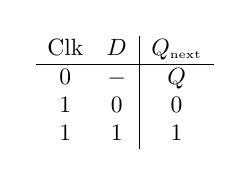
\begin{tikzpicture}
\node[scale=0.85] (TT) at (3,0) {$\begin{array}{cc|c}\mbox{Clk}&D&Q_{\mbox{\tiny{next}}}\\\hline0&-&Q\\1&0&0\\1&1&1\end{array}$};
\end{tikzpicture}
}
\caption{Geklokte D-latch.}
\label{fig:clockedDLatch}
\end{figure}
\paragraph{Set-up- en houdtijd}
Aan de hand van de implementatie van de geklokte D-latch op figuur \ref{fig:clockedDLatch} zullen we de vertragingen van verschillende signalen berekenen:
\begin{equation}
\begin{array}{ccl}
D\rightarrow Q&:&\left\{\begin{array}{lll}
t_{HL}=1.4+1.4=2.8&\ifun&D=0\wedge\mbox{Clk}=1\\
t_{LH}=1+1.4+1.4+1.4=5.2&\ifun&D=1\wedge\mbox{Clk}=1
\end{array}\right.\\\\
D\rightarrow Q_n&:&\left\{\begin{array}{lll}
t_{HL}=1+1.4+1.4=3.8&\ifun&D=0\wedge\mbox{Clk}=1\\
t_{LH}=1.4+1.4+1.4=4.2&\ifun&D=1\wedge\mbox{Clk}=1
\end{array}\right.\\\\
\mbox{Clk}\rightarrow Q&:&\left\{\begin{array}{lll}
t_{HL}=1.4+1.4+1.4=4.2&\ifun&D=0\wedge\mbox{Clk}=1\\
t_{LH}=1.4+1.4=2.8&\ifun&D=1\wedge\mbox{Clk}=1
\end{array}\right.\\\\
\mbox{Clk}\rightarrow Q_n&:&\left\{\begin{array}{lll}
t_{HL}=1.4+1.4+1.4=4.2&\ifun&D=0\wedge\mbox{Clk}=1\\
t_{LH}=1.4+1.4=2.8&\ifun&D=1\wedge\mbox{Clk}=1
\end{array}\right.
\end{array}
\label{eqn:dLatchDelays}
\end{equation}
We kunnen dergelijke vertragingen grafisch weergeven zoals op de tijdsgrafieken op figuur \ref{fig:timebehavDLatch}.
\begin{figure}[hbt]
\centering
\subfigure[Set-up-tijd??]{%TODO: ongeldige toestand op figuur zetten
\begin{tikzpicture}
%\timebehav{5}{-1}{14.5}{6}{1.3}{0/$Q$,1/$R^*$,2/$S^*$,3/$D'$,4/Clk,5/$D$}{5/0/0/1/1,5/1/1/5/1, 4/0/1/2.2/0,4/2.2/0/5/0, 3/0/1/2/0,3/2/0/5/0, 2/0/1/2.4/0,2/2.4/0/3.6/1,2/3.6/1/5/1, 1/0/0/3.4/1,1/3.4/1/5/1, 0/0/0/3.8/1,0/3.8/1/5/1, 5/6/0/7/1,5/7/1/11/1,4/6/1/7.5/0,4/7.5/0/11/0, 3/6/1/8/0,3/8/0/11/0, 2/6/1/8.4/0,2/8.4/0/8.9/1,2/8.9/1/11/1, 1/6/0/9.4/1,1/9.4/1/11/1, 0/6/0/9.8/1,0/9.8/1/11/1}{1/1/5/3,1/1.4/5/2,2/1.4/3/1,2.2/1.4/4/2,2.4/1.4/2/0, 7/1/5/3,7/1.4/5/2,7.5/1.4/4/2,8/1.4/3/1,8.4/1.4/2/0,8.9/1.4/2/0,9.4/1.4/1/0}
%\timebehav{5.00}{-1.00}{6.70}{7}{0.80}{0/$Q_n$,1/$Q$,2/$R^*$,3/$S^*$,4/$D'$,5/Clk,6/$D$}{0/0.00/1/5.20/0, 0/5.20/0/8.00/0, 1/0.00/0/3.80/1, 1/3.80/1/8.00/1, 2/0.00/0/3.40/1, 2/3.40/1/8.00/1, 3/0.00/1/2.40/0, 3/2.40/0/5.40/1, 3/5.40/1/8.00/1, 4/0.00/1/2.00/0, 4/2.00/0/8.00/0, 5/0.00/1/4.00/0, 5/4.00/0/8.00/0, 6/0.00/0/1.00/1, 6/1.00/1/8.00/1}{3.80/1.40/1/0, 2.40/1.40/3/1, 2.00/1.40/4/2, 1.00/1.40/6/3, 4.00/1.40/5/3, 1.00/1.00/6/4};

\timebehav{0.00}{0.00}{6.70}{7}{0.80}{0/$Qn$,1/$Q$,2/$R*$,3/$S*$,4/$Dn$,5/$Clk$,6/$D$}{0/0.00/1/5.20/0, 0/5.20/0/8.00/0, 1/0.00/0/3.80/1, 1/3.80/1/8.00/1, 2/0.00/0/3.40/1, 2/3.40/1/8.00/1, 3/0.00/1/2.40/0, 3/2.40/0/5.40/1, 3/5.40/1/8.00/1, 4/0.00/1/2.00/0, 4/2.00/0/8.00/0, 5/0.00/1/4.00/0, 5/4.00/0/8.00/0, 6/0.00/0/1.00/1, 6/1.00/1/8.00/1}{3.80/1.40/1/0, 2.40/1.40/3/1, 2.00/1.40/4/2, 1.00/1.40/6/3, 4.00/1.40/5/3, 1.00/1.00/6/4};
\timebehav{8.00}{0.00}{6.70}{7}{0.80}{0/$Qn$,1/$Q$,2/$R*$,3/$S*$,4/$Dn$,5/$Clk$,6/$D$}{0/0.00/1/5.20/0, 0/5.20/0/5.70/1, 0/5.70/1/8.00/0, 0/8.00/0/8.00/0, 1/0.00/0/3.80/1, 1/3.80/1/4.30/0, 1/4.30/0/6.60/1, 1/6.60/1/7.10/0, 1/7.10/0/8.00/0, 2/0.00/0/2.90/1, 2/2.90/1/8.00/1, 3/0.00/1/2.40/0, 3/2.40/0/2.90/1, 3/2.90/1/8.00/1, 4/0.00/1/2.00/0, 4/2.00/0/8.00/0, 5/0.00/1/1.50/0, 5/1.50/0/8.00/0, 6/0.00/0/1.00/1, 6/1.00/1/8.00/1}{3.80/1.40/1/0, 4.30/1.40/1/0, 6.60/1.40/1/0, 2.40/1.40/3/1, 2.90/1.40/3/1, 5.20/1.40/0/1, 5.70/1.40/0/1, 1.50/1.40/5/2, 1.00/1.40/6/3, 1.50/1.40/5/3, 1.00/1.00/6/4};
%\timebehav{13.00}{-1.00}{6.70}{7}{0.80}{0/$Q_n$,1/$Q$,2/$R^*$,3/$S^*$,4/$D'$,5/Clk,6/$D$}{0/0.00/1/5.20/0, 0/5.20/0/6.40/1, 0/6.40/1/8.00/0, 0/8.00/0/8.00/0, 1/0.00/0/3.80/1, 1/3.80/1/5.00/0, 1/5.00/0/6.60/1, 1/6.60/1/7.80/0, 1/7.80/0/8.00/0, 2/0.00/0/3.40/1, 2/3.40/1/8.00/1, 3/0.00/1/2.40/0, 3/2.40/0/3.60/1, 3/3.60/1/8.00/1, 4/0.00/1/2.00/0, 4/2.00/0/8.00/0, 5/0.00/1/2.20/0, 5/2.20/0/8.00/0, 6/0.00/0/1.00/1, 6/1.00/1/8.00/1}{3.80/1.40/1/0, 5.00/1.40/1/0, 6.60/1.40/1/0, 2.40/1.40/3/1, 3.60/1.40/3/1, 5.20/1.40/0/1, 6.40/1.40/0/1, 2.00/1.40/4/2, 1.00/1.40/6/3, 2.20/1.40/5/3, 1.00/1.00/6/4};
%\timebehav{13.00}{-6.00}{6.70}{7}{0.80}{0/$Q_n$,1/$Q$,2/$R^*$,3/$S^*$,4/$D'$,5/Clk,6/$D$}{0/0.00/1/5.20/0, 0/5.20/0/6.20/1, 0/6.20/1/8.00/0, 0/8.00/0/8.00/0, 1/0.00/0/3.80/1, 1/3.80/1/4.80/0, 1/4.80/0/6.60/1, 1/6.60/1/7.60/0, 1/7.60/0/8.00/0, 2/0.00/0/3.40/1, 2/3.40/1/8.00/1, 3/0.00/1/2.40/0, 3/2.40/0/3.40/1, 3/3.40/1/8.00/1, 4/0.00/1/2.00/0, 4/2.00/0/8.00/0, 5/0.00/1/2.00/0, 5/2.00/0/8.00/0, 6/0.00/0/1.00/1, 6/1.00/1/8.00/1}{3.80/1.40/1/0, 4.80/1.40/1/0, 6.60/1.40/1/0, 2.40/1.40/3/1, 3.40/1.40/3/1, 5.20/1.40/0/1, 6.20/1.40/0/1, 2.00/1.40/5/2, 2.00/1.40/4/2, 1.00/1.40/6/3, 2.00/1.40/5/3, 1.00/1.00/6/4};
\end{tikzpicture}
\label{fig:timebehavDLatchSetup}
}
\subfigure[Houdtijd??]{%TODO: afwerken
\begin{tikzpicture}
\timebehav{0.00}{0.00}{6.70}{7}{0.80}{0/$Qn$,1/$Q$,2/$R*$,3/$S*$,4/$Dn$,5/$Clk$,6/$D$}{0/0.00/1/5.20/0, 0/5.20/0/7.70/1, 0/7.70/1/8.00/0, 0/8.00/0/8.00/0, 1/0.00/0/3.80/1, 1/3.80/1/6.30/0, 1/6.30/0/6.60/1, 1/6.60/1/8.00/1, 2/0.00/0/3.40/1, 2/3.40/1/8.00/1, 3/0.00/1/2.40/0, 3/2.40/0/4.90/1, 3/4.90/1/8.00/1, 4/0.00/1/2.00/0, 4/2.00/0/4.50/1, 4/4.50/1/8.00/1, 5/0.00/1/4.00/0, 5/4.00/0/8.00/0, 6/0.00/0/1.00/1, 6/1.00/1/3.50/0, 6/3.50/0/8.00/0}{3.80/1.40/1/0, 6.30/1.40/1/0, 6.60/1.40/1/0, 2.40/1.40/3/1, 4.90/1.40/3/1, 5.20/1.40/0/1, 2.00/1.40/4/2, 1.00/1.40/6/3, 3.50/1.40/6/3, 1.00/1.00/6/4, 3.50/1.00/6/4};
\timebehav{8.00}{0.00}{6.70}{7}{0.80}{0/$Qn$,1/$Q$,2/$R*$,3/$S*$,4/$Dn$,5/$Clk$,6/$D$}{0/0.00/1/5.20/0, 0/5.20/0/8.00/0, 1/0.00/0/3.80/1, 1/3.80/1/8.00/1, 2/0.00/0/3.40/1, 2/3.40/1/8.00/1, 3/0.00/1/2.40/0, 3/2.40/0/5.20/1, 3/5.20/1/8.00/1, 4/0.00/1/2.00/0, 4/2.00/0/4.80/1, 4/4.80/1/8.00/1, 5/0.00/1/4.00/0, 5/4.00/0/8.00/0, 6/0.00/0/1.00/1, 6/1.00/1/3.80/0, 6/3.80/0/8.00/0}{3.80/1.40/1/0, 2.40/1.40/3/1, 2.00/1.40/4/2, 1.00/1.40/6/3, 3.80/1.40/6/3, 1.00/1.00/6/4, 3.80/1.00/6/4};
%\timebehav{5}{-1}{14.5}{6}{1.3}{0/$Q$,1/$R^*$,2/$S^*$,3/$D'$,4/Clk,5/$D$}{5/0/1/2.2/0, 4/0/1/1/0, 3/0/0/3.2/1}{1/1/5/3}
\end{tikzpicture}
\label{fig:timebehavDLatchHold}
}
\caption{Tijdsgrafieken van een D-latch.}
\label{fig:timebehavDLatch}
\end{figure}
Deze grafische voorstelling toont twee bekende problemen die veroorzaakt worden door het niet respecteren van twee parameters:
\begin{itemize}
 \item \termen{Set-up-tijd}: De tijd alvorens de het actieve kloksignaal wordt verlaten waarin de waarde op de data-ingang niet meer mag wijzigen. Bij een geklokte $D$-latch zoals op figuur \ref{fig:clockedDLatch} is dit:
\begin{equation}
\begin{array}{cr}
t_{\mbox{\tiny{set-up}}}=t_{pHL}\left(\mbox{inverter}\right)&\mbox{(vertraging van een hoog-naar-laag signaal door een inverter)}
\end{array}
\end{equation}
Figuur \ref{fig:timebehavDLatchSetup} toont twee senarios. Bij het eerste wordt de set-up tijd gerespecteerd, bij het tweede faalt de toekenning. Dit komt omdat bij dit scenario $S^*$ weer hoog wordt alvorens $R^*$ een hoog signaal aanlegt. Indien we de vertragingen van de poorten doorrekenen komen we uit dat de vertraging van aan de inverter een cruciale rol speelt. Dit is ook enigszins logisch: indien we een 0 aan de data-ingang $D$ aanleggen zal gedurende deze periode 1 op zowel de $S$ als $R$ van de geklokte SR-latch worden aangelegd, wat eigenlijk een ongeldige invoer is.
 \item \termen{Houdtijd}: We moeten niet alleen het signaal op tijd aanleggen voor de klok een laag signaal aanlegt. Meestal moeten we het signaal daarna nog een tijdje laten staan om te vermijden dat de latch alsnog een foute waarde aanneemt. Figuur \ref{fig:timebehavDLatchHold} toont opnieuw twee scenarios.??%TODO: afwerken
\end{itemize}
\paragraph{Metastabiliteit}
Een ander probleem dat komt kijken bij latches is de \termen{metastabiliteit}. Dit probleem treed op bij de twee poorten\footnote{NAND- of NOR-implementatie maakt niet uit.} van de SR-latch en dus bijgevolg alle afgeleide latches. Als we bij de NOR-implementatie $\left(S,R\right)=\left(0,0\right)$ aanleggen, of bij een NAND-implementatie $\left(S^*,R^*\right)=\left(1,1\right)$, kunnen we deze poorten modelleren als NOT-poorten zoals op figuur \ref{fig:metastabilityNotGates}.
\begin{figure}[hbt]
\centering
\subfigure[Implementatie.]{
\begin{tikzpicture}[circuit logic US,scale=1.2]
\node[not gate] (NO0) at (0,0.65) {};
\node[not gate] (NO1) at (0,-0.65) {};
\draw (NO1.output) -- (NO1.output -| 0.85,0) node[anchor=west,scale=0.75]{$x$} -- (0.85,-0.4) -- (-0.75,0.4) -- (NO0.input -| -0.75,0) -- (NO0.input);
\draw (NO0.output) -- (NO0.output -| 0.85,0) node[anchor=west,scale=0.75]{$y$} -- (0.85,0.4) -- (-0.75,-0.4) -- (NO1.input -| -0.75,0) -- (NO1.input);
\end{tikzpicture}
\label{fig:metastabilityNotGates}}
\subfigure[Transfer-functies.]{
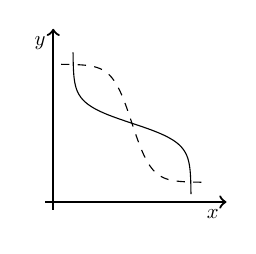
\begin{tikzpicture}
\draw[thick,->] (-0.1,0) -- (2.2,0) node[anchor=north east,scale=0.75]{$x$};
\draw[thick,->] (0,-0.1) -- (0,2.2) node[anchor=north east,scale=0.75]{$y$};
\draw [samples=100,smooth,domain=0.1:1.9,variable=\x,dashed] plot (\x,{1.75-1.5/(1+exp(-8*\x+8))});
\draw [samples=100,smooth,domain=0.1:1.9,variable=\x] plot ({1.75-1.5/(1+exp(-8*\x+8))},\x);
\pdot{1,1};
\pdot{0.2538,1.7462};
\pdot{1.7462,0.2538};
\end{tikzpicture}
\label{fig:metastabilityNotFunctions}}
\subfigure[Bal-en-heuvel-analogie.]{
\begin{tikzpicture}
\draw[pattern=vertical lines] [samples=100,smooth,domain=-2:2,variable=\x] plot (\x,{cos(114.591559029*\x)}) -- (2,-1.3) -- (-2,-1.3) -- cycle;
\filldraw[fill=black!20,draw=black] (0,1.125) circle (0.125 cm);
\filldraw[fill=black!20,draw=black] (-1.570796327,-0.875) circle (0.125 cm);
\filldraw[fill=black!20,draw=black] (1.570796327,-0.875) circle (0.125 cm);
\end{tikzpicture}
\label{fig:metastabilityAnalogy}}
\caption{Metastabiliteit.}
\label{fig:metastability}
\end{figure}
Indien we deze schakeling logisch analyseren zien we twee mogelijke stabiele oplossingen: waarbij ofwel $x$ ofwel $y$ 1 is, en de andere 0. Deze waarden zijn ook de enige die we beschouwen indien we de NOT-poort louter als logisch component zien. We implementeren deze poorten echter met behulp van transistoren, bijgevolg behoudt de poort een zeker analoog karakter. Op de grafiek op figuur \ref{fig:metastabilityNotFunctions} geven we de transfer-functie van de twee NOT-poorten weer. De stippelijn geeft de transfer-functie van de bovenste NOT-poort weer, de volle lijn de onderste. We zien zoals verwacht de twee \termen{stabiele toestanden}. We bemerken echter ook een \termen{metastabiele toestand}. Op het moment dat op $x$ of $y$ een kleine hoeveelheid ruis wordt aangebracht zullen de poorten dit effect versterken en zal zal de schakeling in een stabiele toestand terechtkomen. Het probleem is echter dat we uiteraard niet weten hoelang dit zal duren. We gaan er echter vanuit dat de kans dat na een bepaald tijdstip er nog onvoldoende ruis is opgetreden Poisson-verdeeld is\footnote{De meeste kansverdelingen op het voorkomen van een gebeurtenis zijn Poisson-verdeeld.}. We formaliseren dus tot:
\begin{equation}
p\left(\mbox{nog in metastabiele toestand na $t$}\right)=e^{-t/\tau}
\end{equation}
De \termen{tijdsconstante $\tau$} is hierbij afhangen van twee factoren:
\begin{itemize}
 \item De hoeveelheid ruis: hoe meer ruis hoe lager de tijdsconstante.
 \item De stijlheid van de curves rond de metastabiele toestand: hoe stijler hoe lager de tijdsconstante.
\end{itemize}
Een latch kan in een metastabiele toestand komen door een zogenaamde \termen{marginale triggering}: een schending van de set-up- of houdtijd of van de minimale pulsbreedte\footnote{De tijd dat een signaal wordt aangelegd.}. In deze gevallen kan een overgang tussen twee stabiele toestanden worden onderbroken. Indien dit gebeurt op het moment dat men net voorbij de metastabiele toestand passeert treed dit probleem op. Een latch komt dan ook bij elke overgang kortstondig in een metastabiele toestand. Ook een tijdje in een metastabiele toestand blijven is geen probleem. Zolang deze toestand niet meer actief is wanneer we het signaal gaan gebruiken zullen er geen problemen optreden. Een populaire voorstelling van metastabiliteit is de zogenaamde \termen{bal-en-heuvel-analogie}. In deze analogie beschrijven we een heuvel zoals op figuur \ref{fig:metastabilityAnalogy}. Een bal kan op deze heuvel in drie toestanden een evenwicht bereiken: twee toestanden in een dal (passief evenwicht) en een metastabiele toestand op de heuvel (actief evenwicht). Bij asynchrone circuits is metastabiliteit een veel voorkomend fenomeen. Zeker wanneer de klokfrequentie geen veelvoud is van de frequentie waarmee de ingang omwisselt. In dat geval bestaat de oplossing van het probleem eerder uit ``hoe ga ik om met metastabiliteit?'', in plaats van ``hoe los ik de metastabiliteit op?''.
\subsubsection{De flipflop}
Latches kunnen we gebruiken bij het opslaan van \'e\'en bit. Indien we een geklokte latch aan een kloksignaal hangen zijn er twee toestanden afhankelijk van het niveau van het kloksignaal:
\begin{itemize}
 \item Indien het kloksignaal hoog is $\mbox{Clk}=1$ is de latch \termen{transparant}. De latch neemt de waarde over die aan de ingang staat.
 \item Indien het kloksignaal laag is $\mbox{Clk}=0$ onthoud de latch de laatste waarde die aan de ingang stond toen de latch transparant was.
\end{itemize}
Latches geven echter problemen op het moment we verschillende latches na elkaar willen hangen. In dat geval zullen immers alle latches transparant zijn op hetzelfde moment. Hierdoor zal de laatste latch de waarde aannemen die op de eerste latch wordt aangelegd\footnote{Bij een groot aantal latches zal het signaal door vertragingen en set-up- en houdtijd uiteraard maar door een beperkt aantal latches in \'e\'en klokflank propageren.}. Dit probleem wordt ook wel het \termen{transparantie-probleem} genoemd. Meestal willen we echter bij een sequentie van een aantal geheugencomponenten afdwingen dat de informatie door \'e\'en geheugencomponent per klokflank propageert. De flipflop is een geheugencomponent die in tegenstelling tot de latch \termen{flankgevoelig} is. Dit betekent dat de flipflop enkel transparant is op het moment dat de klok van 0 naar 1 gaat, in tegenstelling tot een latch die transparant is gedurdende de volledige periode dat de klok hoog is. Om dit te realiseren zijn er doorgaans twee methodes:
\begin{itemize}
 \item De \termen{master-slave flipflop}.
 \item De \termen{edge-triggered flipflop}.
\end{itemize}
We zullen deze twee verschillende technieken in de volgende paragrafen toelichten.
\paragraph{Master-slave flipflop}
Een master-slave flipflop maakt gebruik van twee latches die beurtelings transparant zijn. De master (eerste latch) is transparant wanneer het kloksignaal laag is, de tweede latch is transparant bij een hoog kloksignaal. Gegroepeerd vormen we dus een geheugen die de laatste waarde opslaat die aan de ingang stond op het moment dat het kloksignaal laag was, en deze verder propageert op het moment dat het kloksignaal hoog is. Figuur \ref{fig:masterSlaveFlipflop} toont dit concept samen met een tijdsgrafiek.??
\begin{figure}[hbt]
\centering
\subfigure[Implementatie.]{
\begin{tikzpicture}[circuit logic US]
\def\cly{-1.125};
\def\nff{2};
\def\nffd{1};
\def\nffi{3};
\foreach\x in {0,...,\nff} {
  \filldraw[draw=black,dashed,fill=black!20] (4*\x-1.125,\cly-0.125) rectangle (4*\x+2.425,1.25);
  \node[cldlatchmaster,scale=0.75] (M\x) at (4*\x,0) {};
  \node[cldlatch,scale=0.75] (S\x) at (4*\x+1.75,0) {};
  \draw (M\x.Clk) -| (4*\x-1,\cly);
  \node[anchor=south] (Mt\x) at (M\x.north) {Master};
  \node[anchor=south] (St\x) at (S\x.north) {Slave};
  \pdot{4*\x-1,\cly};
  \draw (M\x.Q) -- (S\x.D);
  \draw (S\x.Clk) -| (4*\x+0.75,\cly);
}
\foreach\xd/\x in {0/1,1/2} {
  \draw (S\xd.Q) to node[midway,above,scale=0.75]{$Q_{\x}$} (M\x.D);
  \pdot{0.75+4*\xd,\cly};
}
\draw (0.75+4*\nff,\cly) -- (-1.5,\cly) node[scale=0.75,anchor=east]{Clk};
\draw (M0.D) -- (M0.D -| -1.5,0) node[scale=0.75,anchor=east]{$D$};
\draw (S\nff.Q) -- (S\nff.Q -| 4*\nff+3,0) node[scale=0.75,anchor=west]{$Q_{\nffi}$};
\end{tikzpicture}}
\subfigure[Interface]{
\begin{tikzpicture}
\node[dff] (DFF) at (0,0) {};
\end{tikzpicture}}
\caption{Master-slave flipflop.}
\label{fig:masterSlaveFlipflop}
\end{figure}
\paragraph{Edge-triggered flipflop}
Een Edge-trigger flipflop maakt gebruik van een structuur die we kunnen groeperen als drie latches. Deze schakeling stelt ons in staat om om het signaal op te slaan die aan de ingang staat op het moment dat de klok van 0 naar 1 gaat. Figuur \ref{fig:edgeTriggeredFlipflop} toont een basis en meer uitgebreide implementatie samen met een tijdsgrafiek.
\begin{figure}[hbt]
\centering
\subfigure[Basisimplementatie.]{
\begin{tikzpicture}[circuit logic US]
\def\dx{-1.75};
\def\dy{1.35};
\node[nand gate] (NA10) at (0,0.65) {};
\node[nand gate] (NA11) at (0,-0.65) {};
\draw (NA11.output -| 0.85,0) -- (0.85,-0.4) -- (-0.75,0.4) -- (NA10.input 2 -| -0.75,0) -- (NA10.input 2);
\draw (NA10.output -| 0.85,0) -- (0.85,0.4) -- (-0.75,-0.4) -- (NA11.input 1 -| -0.75,0) -- (NA11.input 1);
\draw (NA10.output) -- (NA10.output -| 1.1,0) node[anchor=west,scale=0.75]{$Q_n$};
\draw (NA11.output) -- (NA11.output -| 1.1,0) node[anchor=west,scale=0.75]{$Q$};
\pdot{NA10.output -| 0.85,0};
\pdot{NA11.output -| 0.85,0};
\node[nand gate] (NA01) at (NA10.input 1 -| \dx,0) {};
\node[nand gate,inputs={normal,normal,normal}] (NA02) at (NA11.input 2 -| \dx,0) {};
\draw (NA01.output) -- (NA10.input 1);
\draw (NA02.output) -- (NA11.input 2);
\node[nand gate] (NA00) at (\dx,2) {};
\node[nand gate] (NA03) at (\dx,-2) {};
\draw (NA01.output -| \dx+0.85,0) -- (\dx+0.85,\dy-0.3) -- (\dx-0.75,\dy+0.3) -- (NA00.input 2 -| \dx-0.75,0) -- (NA00.input 2);
\draw (NA00.output) -- (NA00.output -| \dx+0.85,0) -- (\dx+0.85,\dy+0.3) -- (\dx-0.75,\dy-0.3) -- (NA01.input 1 -| \dx-0.75,0) -- (NA01.input 1);
\draw (NA03.output) -- (NA03.output -| \dx+0.85,0) -- (\dx+0.85,-\dy-0.3) -- (\dx-0.75,-\dy+0.3) -- (NA02.input 3 -| \dx-0.75,0) -- (NA02.input 3);
\draw (NA02.output -| \dx+0.85,0) -- (\dx+0.85,-\dy+0.4) -- (\dx-0.75,-\dy-0.4) -- (NA03.input 1 -| \dx-0.75,0) -- (NA03.input 1);
\draw (NA01.output -| \dx+0.85,0) -- (\dx+0.85,0.4) -- (\dx-0.75,-0.4) -- (NA02.input 1 -| \dx-0.75,0) -- (NA02.input 1);
\draw (NA00.output -| \dx+0.85,0) node[anchor=west,scale=0.75]{$A$};
\pdot{NA01.output -| \dx+0.85,0};
\draw (NA01.output -| \dx+0.85,0) node[anchor=south west,scale=0.75]{$S^*$};
\pdot{NA02.output -| \dx+0.85,0};
\draw (NA02.output -| \dx+0.85,0) node[anchor=north west,scale=0.75]{$R^*$};
\pdot{NA02.input 3 -| \dx-0.75,0};
\draw (NA03.output -| \dx+0.85,0) node[anchor=west,scale=0.75]{$B$};
\draw (NA02.input 3 -| \dx-0.75,0) -- ++(-0.5,0) |- (NA00.input 1);
\draw (NA02.input 2) -- (NA02.input 2 -| \dx-0.75,0) -- ++(-0.25,0) |- (NA01.input 2);
\draw (\dx-1,0) -- ++(-0.5,0) node[anchor=east,scale=0.75]{Klok Clk};
\pdot{\dx-1,0};
\draw (NA03.input 2) -- (NA03.input 2 -| \dx-1.5,0) node[anchor=east,scale=0.75]{$D$};
\end{tikzpicture}
\label{fig:edgeTriggeredFlipflopBasic}}
\subfigure[Uitgebreide implementatie.]{
\begin{tikzpicture}[circuit logic US]
\def\dx{-1.75};
\def\dy{1.35};
\node[nand gate,inputs={normal,normal,normal}] (NA10) at (0,0.65) {};
\node[nand gate,inputs={normal,normal,normal}] (NA11) at (0,-0.65) {};
\draw (NA11.output -| 0.85,0) -- (0.85,-0.3) -- (-0.75,0.3) -- (NA10.input 3 -| -0.75,0) -- (NA10.input 3);
\draw (NA10.output -| 0.85,0) -- (0.85,0.3) -- (-0.75,-0.3) -- (NA11.input 1 -| -0.75,0) -- (NA11.input 1);
\draw (NA10.output) -- (NA10.output -| 1.1,0) node[anchor=west,scale=0.75]{$Q_n$};
\draw (NA11.output) -- (NA11.output -| 1.1,0) node[anchor=west,scale=0.75]{$Q$};
\pdot{NA10.output -| 0.85,0};
\pdot{NA11.output -| 0.85,0};
\node[nand gate,inputs={normal,normal,normal}] (NA01) at (NA10.input 2 -| \dx,0) {};
\node[nand gate,inputs={normal,normal,normal}] (NA02) at (NA11.input 2 -| \dx,0) {};
\draw (NA01.output) -- (NA10.input 2);
\draw (NA02.output) -- (NA11.input 2);
\node[nand gate,inputs={normal,normal,normal}] (NA00) at (\dx,2) {};
\node[nand gate,inputs={normal,normal,normal}] (NA03) at (\dx,-2) {};
\draw (NA01.output -| \dx+0.85,0) -- (\dx+0.85,\dy-0.3) -- (\dx-0.75,\dy+0.3) -- (NA00.input 3 -| \dx-0.75,0) -- (NA00.input 3);
\draw (NA00.output) -- (NA00.output -| \dx+0.85,0) -- (\dx+0.85,\dy+0.3) -- (\dx-0.75,\dy-0.3) -- (NA01.input 1 -| \dx-0.75,0) -- (NA01.input 1);
\draw (NA03.output) -- (NA03.output -| \dx+0.85,0) -- (\dx+0.85,-\dy-0.3) -- (\dx-0.75,-\dy+0.3) -- (NA02.input 3 -| \dx-0.75,0) -- (NA02.input 3);
\draw (NA02.output -| \dx+0.85,0) -- (\dx+0.85,-\dy+0.3) -- (\dx-0.75,-\dy-0.3) -- (NA03.input 1 -| \dx-0.75,0) -- (NA03.input 1);
\draw (NA01.output -| \dx+0.85,0) -- (\dx+0.85,0.4) -- (\dx-0.75,-0.4) -- (NA02.input 1 -| \dx-0.75,0) -- (NA02.input 1);
\pdot{NA01.output -| \dx+0.85,0};
\pdot{NA02.output -| \dx+0.85,0};
\pdot{NA02.input 3 -| \dx-0.75,0};
\draw (NA02.input 3 -| \dx-0.75,0) -- ++(-0.5,0) |- (NA00.input 2);
\draw (NA02.input 2) -- (NA02.input 2 -| \dx-0.75,0) -- ++(-0.25,0) |- (NA01.input 2);
\draw (\dx-1,0) -- ++(-0.75,0) node[anchor=east,scale=0.75]{Klok Clk};
\pdot{\dx-1,0};
\draw (NA03.input 2) -- (NA03.input 2 -| \dx-1.75,0) node[anchor=east,scale=0.75]{$D$};
\coordinate (CLRI) at (\dx-1.75,-2.5);
\coordinate (PRI) at (\dx-1.75,2.5);
\draw (PRI) node[anchor=east,scale=0.75]{Preset $\mbox{PR}^*$} -- (PRI -| -0.75,0) |- (NA10.input 1);
\draw (CLRI) node[anchor=east,scale=0.75]{Clear $\mbox{CLR}^*$} -- (CLRI -| -0.75,0) |- (NA11.input 3);
\draw (PRI -| \dx-0.75,0) |- (NA00.input 1);
\pdot{PRI -| \dx-0.75,0};
\draw (CLRI -| \dx-1.5,0) |- (NA03.input 3);
\pdot{CLRI -| \dx-1.5,0};
\draw (\dx-1.5,0 |- NA03.input 3) |- (NA01.input 3);
\pdot{\dx-1.5,0 |- NA03.input 3};
\end{tikzpicture}
\label{fig:edgeTriggeredFlipflopExtended}}
\subfigure[Tijdsgrafiek]{\begin{tikzpicture}
\timebehav{5.00}{-1.00}{8.50}{8}{0.75}{0/$Qn$,1/$Q$,2/$S^*$,3/$R^*$,4/$A$,5/$B$,6/$D$,7/Clk}{0/0.00/1/1.55/0, 0/1.55/0/3.88/1, 0/3.88/1/6.55/0, 0/6.55/0/8.88/1, 0/8.88/1/11.48/1, 1/0.00/0/1.30/1, 1/1.30/1/4.13/0, 1/4.13/0/6.30/1, 1/6.30/1/9.13/0, 1/9.13/0/11.48/0, 2/0.00/1/1.05/0, 2/1.05/0/2.30/1, 2/2.30/1/6.05/0, 2/6.05/0/7.30/1, 2/7.30/1/11.48/1, 3/0.00/1/3.63/0, 3/3.63/0/4.88/1, 3/4.88/1/8.63/0, 3/8.63/0/9.88/1, 3/9.88/1/11.13/0, 3/11.13/0/11.48/0, 4/0.00/0/0.68/1, 4/0.68/1/3.18/0, 4/3.18/0/5.38/1, 4/5.38/1/7.55/0, 4/7.55/0/11.48/0, 5/0.00/1/0.43/0, 5/0.43/0/2.93/1, 5/2.93/1/5.13/0, 5/5.13/0/6.68/1, 5/6.68/1/11.48/1, 6/0.00/0/0.18/1, 6/0.18/1/2.68/0, 6/2.68/0/3.93/1, 6/3.93/1/6.43/0, 6/6.43/0/11.48/0, 7/0.00/0/0.80/1, 7/0.80/1/2.05/0, 7/2.05/0/3.30/1, 7/3.30/1/4.55/0, 7/4.55/0/5.80/1, 7/5.80/1/7.05/0, 7/7.05/0/8.30/1, 7/8.30/1/9.55/0, 7/9.55/0/10.80/1, 7/10.80/1/11.48/1}{1.30/0.25/1/0, 3.63/0.25/3/0, 6.30/0.25/1/0, 8.63/0.25/3/0, 1.05/0.25/2/1, 3.88/0.25/0/1, 6.05/0.25/2/1, 8.88/0.25/0/1, 0.80/0.25/7/2, 2.05/0.25/7/2, 5.80/0.25/7/2, 7.05/0.25/7/2, 3.30/0.32/7/3, 4.55/0.32/7/3, 8.30/0.32/7/3, 9.55/0.32/7/3, 10.80/0.32/7/3, 0.43/0.25/5/4, 2.93/0.25/5/4, 5.13/0.25/5/4, 7.30/0.25/2/4, 0.18/0.25/6/5, 2.68/0.25/6/5, 4.88/0.25/3/5, 6.43/0.25/6/5};
\end{tikzpicture}
}
\caption{Edge-triggered flipflop.}
\label{fig:edgeTriggeredFlipflop}
\end{figure}
In de meer uitgebreide versie zijn er naast de data- en klokingang ook nog twee andere ingangen beschreven:
\begin{itemize}
 \item \termen{Preset $\mbox{PR}^*$}: Indien dit signaal laag wordt, slaan we asynchroon een 1 op in de flipflop.
 \item \termen{Clear $\mbox{CLR}^*$}: Indien dit signaal laag wordt, slaan we asynchroon een 0 op in de flipflop. 
\end{itemize}
Deze twee signalen worden ook wel de \termen{asynchrone set en reset} genoemd. Ze zijn asynchroon omdat ze onafhankelijk van de toestand van de klok een waarde in het geheugen kunnen inbrengen, deze eigenschap wordt bijvoorbeeld gebruikt om bij het opkomen van de stroom in de elektronica de flipflop in een gekende toestand te brengen\footnote{Bij het opkomen van de stroom zal de flipflop of latch immers een waarde aannemen afhankelijk van de ruis en minimale verschillen in poortvertragingen.}.??
\subsubsection{Types flipflops}
\label{sss:typesFlipflops}
Er bestaan analoog aan de latches ook verschillende types flipflops. Hierbij is niet de klokaansturing variabel, maar de manier hoe data ingelezen wordt. Denk bijvoorbeeld aan het verschil tussen een SR-latch en D-latch. Elk type flipflop kunnen we karakteriseren aan de hand van twee tabellen:
\begin{itemize}
 \item De \termen{karakteristieke tabel}: deze tabel gebruikt men bij de implementatie van de flipflops. Het toont aan de linkerkant de ingangen, en aan de rechterkant geeft het weer hoe er op deze ingangen wordt ingespeeld. 
 \item De \termen{excitatietabel}: deze tabel beschrijft de verschillende vormen van gedrag van het component aan de linkerkant, en aan de rechterkant hoe we dit gedrag kunnen verwezenlijken met de ingangen.
\end{itemize}
Deze twee tabellen zijn niet strikt het omgekeerde omdat de excitatietabel een kolom voorziet voor $Q$ en $Q_{\mbox{\tiny{next}}}$, terwijl de karakteristieke tabel uitsluitend \'e\'en kolom aan de rechterkant voorziet. In de volgende paragrafen zullen we de verschillende types flipflops bespreken met hun karakteristieke- en excitatietabel.
\paragraph{SR-flipflop} De \termen{SR-flipflop} ofwel \termen{set-reset flipflop} werkt volledig analoog aan een SR-latch, alleen verandert de waarde uitsluitend op het moment dat de klok van een laag signaal naar een hoog signaal gaat. De karakteristieke tabel is dan ook volledig equivalent met deze van de SR-latch op figuur \ref{fig:setResetLatch}. Figuur \ref{fig:setResetFlipflop} toont de interface en de karakteristieke- en excitatietabel van de SR-flipflop.
\begin{figure}[hbt]
\centering
\begin{tikzpicture}
\node[srff,anchor=west] (I) at (0,0) {};
\node (KT) at (8.5,0) {$\begin{array}{cc|c}
S&R&Q_{\mbox{\tiny{next}}}\\\hline
0&0&Q\\
0&1&0\\
1&0&1\\
1&1&\mbox{N/A}
\end{array}$};
\node[anchor=east] (ET) at (14,0) {$\begin{array}{cc|cc}
Q&Q_{\mbox{\tiny{next}}}&S&R\\\hline
0&0&0&-\\
0&1&1&0\\
1&0&0&1\\
1&1&-&0\\
\end{array}$};
\node[anchor=north] (IT) at (I.south) {Symbool};
\node[anchor=north] (KTT) at (KT.south |- IT.north) {Karakteristieke tabel};
\node[anchor=north] (ETT) at (ET.south |- IT.north) {Excitatietabel};
\end{tikzpicture}
\caption{Set-reset flipflop.}
\label{fig:setResetFlipflop}
\end{figure}
\paragraph{D-flipflop} Ook de \termen{data-flipflop} of \termen{D-flipflop} is conceptueel equivalent aan zijn latch tegenhanger. Op het moment dat de klok van laag naar hoog gaat, zal het signaal dat aan de data-ingang $D$ staat in het geheugen worden geladen. Hierdoor is het bouwen van schakelingen met D-flipflops meestal zeer eenvoudig. Merk dus op dat elk signaal slechts \'e\'en klokperiode bewaard wordt. Figuur \ref{fig:dataFlipflop} toont het symbool samen met de karakteristieke- en excitatietabel.
\begin{figure}[hbt]
\centering
\begin{tikzpicture}
\node[dff,anchor=west] (I) at (0,0) {};
\node (KT) at (8.5,0) {$\begin{array}{c|c}
D&Q_{\mbox{\tiny{next}}}\\\hline
0&0\\
1&1
\end{array}$};
\node[anchor=east] (ET) at (14,0) {$\begin{array}{cc|c}
Q&Q_{\mbox{\tiny{next}}}&D\\\hline
0&0&0\\
0&1&1\\
1&0&0\\
1&1&1\\
\end{array}$};
\node[anchor=north] (IT) at (I.south) {Symbool};
\node[anchor=north] (KTT) at (KT.south |- IT.north) {Karakteristieke tabel};
\node[anchor=north] (ETT) at (ET.south |- IT.north) {Excitatietabel};
\end{tikzpicture}
\caption{Data-flipflop.}
\label{fig:dataFlipflop}
\end{figure}
\paragraph{T-flipflop} Een nieuwe variant is de zogenaamde \termen{toggle-flipflop} ofwel \termen{T-flipflop}. De toggle-flipflop heeft een `toggle'-ingang $T$. Indien deze ingang bij een stijgende klokflank hoog is, zal de flipflop het omgekeerde van zijn huidige waarde opslaan, de zogenaamde `\termen{toggle}'-operatie. Indien $T=0$, blijft opgeslagen toestand dezelfde. We kunnen een toggle-flipflop bouwen met behulp van een data-flipflop en een XOR-poort. Figuur \ref{fig:toggleFlipflop} toont het symbool, een mogelijke implementatie en de karakteristieke- en excitatietabel van de T-flipflop.
\begin{figure}[hbt]
\centering
\begin{tikzpicture}[circuit logic US]
\node[tff,anchor=west] (I) at (0,0) {};
\begin{scope}[xshift=4.5cm]
\filldraw[draw=black,dashed,fill=black!20] (-1.55,-1.1) rectangle (1.55,1.1);
\node[dff,scale=0.7] (DFF) at (0.65,0) {};
\node[xor gate,scale=0.7] (X) at (DFF.D -| -0.65,0) {};
\draw (X.output) -- (DFF.D);
\draw (X.input 1) -- ++(-0.2,0) |- (1.35,0.9) |- (DFF.Q);
\pdot{DFF.Q -| 1.35,0};
\draw (DFF.Q -| 1.35,0) -- (DFF.Q -| 1.75,0) node[scale=0.75,anchor=west]{$Q$};
\draw (DFF.Qn) -- (DFF.Qn -| 1.75,0) node[scale=0.75,anchor=west]{$Q_n$};
\draw (DFF.Clk) -- (DFF.Clk -| -1.75,0) node[scale=0.75,anchor=east]{Clk};
\draw (X.input 2) -- (X.input 2 -| -1.75,0) node[scale=0.75,anchor=east]{$T$};
\end{scope}
\node (KT) at (8.5,0) {$\begin{array}{c|c}
T&Q_{\mbox{\tiny{next}}}\\\hline
0&Q\\
1&Q'\\
\end{array}$};
\node[anchor=east] (ET) at (14,0) {$\begin{array}{cc|c}
Q&Q_{\mbox{\tiny{next}}}&T\\\hline
0&0&0\\
0&1&1\\
1&0&1\\
1&1&0\\
\end{array}$};
\node[anchor=north] (IT) at (I.south) {Symbool};
\node[anchor=north] (IMT) at (4.5,0 |- IT.north) {Implementatie};
\node[anchor=north] (KTT) at (KT.south |- IT.north) {Karakteristieke tabel};
\node[anchor=north] (ETT) at (ET.south |- IT.north) {Excitatietabel};
\end{tikzpicture}
\caption{Toggle-flipflop.}
\label{fig:toggleFlipflop}
\end{figure}
\paragraph{JK-flipflop} De \termen{JK-flipflop} of voluit \termen{Jack Kilby-flipflop}\footnote{Genoemd naar Jack Kilby (1923-2005), Amerikaans natuurkundige en nobelprijswinnaar.} is een combinatie van de set-reset flipflop en de toggle-flipflop. Bij een SR-flipflop komen we immers in een ongeldige toestand indien we aan de ingangen $\left(S,R\right)=\left(1,1\right)$. De JK-flipflop lost dit probleem op door in dat geval een toggle-operatie uit te voeren op het geheugenelement, zoals te zien op de karakteristieke tabel op figuur \ref{fig:jackKilbyFlipflop}. We kunnen een JK-flipflop realiseren met behulp van een SR-flipflop waarbij:
\begin{equation}
\left\{\begin{array}{l}
S=J\cdot Q'\\
R=K\cdot Q
\end{array}\right.
\end{equation}
JK-flipflops worden vooral gebruikt om goedkopere schakelingen te synthetiseren. Deze eigenschap kunnen we afleiden uit de vele don't cares in de excitatietabel.
\begin{figure}[hbt]
\centering
\begin{tikzpicture}[circuit logic US]
\node[jkff,anchor=west] (I) at (0,0) {};
\begin{scope}[xshift=4.5cm]
\filldraw[draw=black,dashed,fill=black!20] (-1.55,-1.1) rectangle (1.55,1.1);
\node[srff,scale=0.7] (SRFF) at (0.65,0) {};
\node[and gate,scale=0.7] (A0) at (SRFF.S -| -0.65,0) {};
\node[and gate,scale=0.7] (A1) at (SRFF.R -| -0.65,0) {};
\draw (A0.output) -- (SRFF.S);
\draw (A1.output) -- (SRFF.R);
\draw (A0.input 2) -- ++(-0.2,0) |- (1.35,-0.9) |- (SRFF.Qn);
\draw (A1.input 1) -- ++(-0.4,0) |- (1.35,0.9) |- (SRFF.Q);
\pdot{SRFF.Q -| 1.35,0};
\pdot{SRFF.Qn -| 1.35,0};
\draw (SRFF.Q -| 1.35,0) -- (SRFF.Q -| 1.75,0) node[scale=0.75,anchor=west]{$Q$};
\draw (SRFF.Qn) -- (SRFF.Qn -| 1.75,0) node[scale=0.75,anchor=west]{$Q_n$};
\draw (SRFF.Clk) -- (SRFF.Clk -| -1.75,0) node[scale=0.75,anchor=east]{Clk};
\draw (A0.input 1) -- (A0.input 1 -| -1.75,0) node[scale=0.75,anchor=east]{$J$};
\draw (A1.input 2) -- (A1.input 2 -| -1.75,0) node[scale=0.75,anchor=east]{$K$};
\end{scope}
\node (KT) at (8.5,0) {$\begin{array}{cc|c}
J&K&Q_{\mbox{\tiny{next}}}\\\hline
0&0&Q\\
0&1&0\\
1&0&1\\
1&1&Q'
\end{array}$};
\node[anchor=east] (ET) at (14,0) {$\begin{array}{cc|cc}
Q&Q_{\mbox{\tiny{next}}}&J&K\\\hline
0&0&0&-\\
0&1&1&-\\
1&0&-&1\\
1&1&-&0\\
\end{array}$};
\node[anchor=north] (IT) at (I.south) {Symbool};
\node[anchor=north] (IMT) at (4.5,0 |- IT.north) {Implementatie};
\node[anchor=north] (KTT) at (KT.south |- IT.north) {Karakteristieke tabel};
\node[anchor=north] (ETT) at (ET.south |- IT.north) {Excitatietabel};
\end{tikzpicture}
\caption{Jack-Kilby flipflop.}
\label{fig:jackKilbyFlipflop}
\end{figure}
\paragraph{Overzicht} We bundelen vervolgens al de latches en flipflops in figuur \ref{fig:latchFlipflopOverview}. Indien een cel leeg is bij dit overzicht is er geen realisatie mogelijk. Zo kunnen we onmogelijk een toggle-latch bouwen: deze zou immers bij een actief kloksignaal continue inverteren, waardoor het uiteindelijke resultaat onvoorspelbaar is. We kunnen elke flipflop verrijken met de assynchrone preset en clear ingangen. Verder bestaan er ook nog varianten van deze componenten waarbij we eerst een negatie toepassen op de ingang. In dat geval plaatsen we een cirkel bij deze ingang. Indien we een negatie toepassen op de klokingang bij een flipflop zal de flipflop dus de waarde memoriseren bij een falling edge, in plaats van een rising edge.
\begin{figure}[hbt]
\centering
\begin{tikzpicture}[decoration={brace}]
\def\dx{3};
\def\dy{-2.5};
\def\ya{0.5*\dy+0.25};
\def\xa{0.5*\dx-0.25};
\node (T0) at (\dx,\ya) {\textbf{Set-Reset (SR)}};
\node (T1) at (2*\dx,\ya) {\textbf{Data (D)}};
\node (T2) at (3*\dx,\ya) {\textbf{Toggle (T)}};
\node (T3) at (4*\dx,\ya) {\textbf{Jack Kilby (JK)}};
\node[rotate=90] (C0) at (\xa,\dy) {\textbf{Ongeklokt}};
\node[rotate=90] (C1) at (\xa,2*\dy) {\textbf{Geklokt}};
\node[rotate=90] (C2) at (\xa,3*\dy) {\textbf{Flankgeklokt}};
\foreach \i in {1,2,3} {
  \draw[thin,dashed] (0.5*\dx+\i*\dx,0 |- T0.north) -- (0.5*\dx+\i*\dx,3.5*\dy);
}
\foreach \i in {1,2} {
  \draw[thin,dashed] (0,0.5*\dy+\i*\dy -| C0.north) -- (4.5*\dx,0.5*\dy+\i*\dy);
}
\draw[very thick] (T0.south -| C0.south) -- (T0.north -| C0.south) -- (4.5*\dx,0 |- T0.north) -- (4.5*\dx,3.5*\dy) -- (0,3.5*\dy -| C2.north) -- (T0.south -| C0.north) -- (T0.south -| C0.south);
\draw[very thick] (4.5*\dx,0 |- T0.south) -- (T0.south -| C0.south) -- (0,3.5*\dy -| C0.south);
\draw [decorate,thick] (4.5*\dx+0.25,0 |- T0.south) -- (4.5*\dx+0.25,2.5*\dy);
\node[rotate=-90,anchor=south] (G0) at (4.5*\dx+0.5,1.5*\dy) {\textbf{Latch}};
\draw [decorate,thick] (4.5*\dx+0.25,2.5*\dy) -- (4.5*\dx+0.25,3.5*\dy);
\node[rotate=-90,anchor=south] (G1) at (4.5*\dx+0.5,3*\dy) {\textbf{Flipflop}};
\foreach\i/\j/\dj/\t/\tx in {1/1/-1/srlatch/NOR,1/1/1/srlatchnand/NAND, 2/1/0/clsrlatch/,2/2/0/cldlatch/, 3/1/-1/srff/Basis,3/1/1/srffx/Uitgebreid,3/2/-1/dff/Basis,3/2/1/dffx/Uitgebreid,3/3/-1/tff/Basis,3/3/1/tffx/Uitgebreid,3/4/-1/jkff/Basis,3/4/1/jkffx/Uitgebreid} {
  \node[scale=0.75,\t] (P) at (\j*\dx+\dj*0.22*\dx,\i*\dy) {};
  \draw(P.south) node[anchor=north,scale=0.75]{\tx};
}
\end{tikzpicture}
\caption{Overzicht van de interfaces van geheugencomponenten.}
\label{fig:latchFlipflopOverview}
\end{figure}
\subsection{Registers}
\label{ss:registers}
\paragraph{Register}Een flipflop kan \'e\'en bit opslaan voor \'e\'en of meerdere klokflanken. Meestal willen we echter meerdere bits opslaan om bijvoorbeeld een getal voor te stellen. Dit kunnen we doen door middel van verschillende flipflops die elk een individuele bit opslaan. Een \termen{register} is in dat opzicht eigenlijk ook een $n$-flipflop. Omdat we vaak meerdere bits opslaan defini\"eren we dus het registercomponent. Een register neemt enige functionaliteit weg van de flipflops: zo kunnen we niet beslissen dat een individuele flipflop een bit aan de ingang opslaat, en de andere flipflops niet. Desalniettemin maken ze schema's eenvoudiger en worden registers op chipniveau verkocht. Verder biedt een dergelijk chip naast geheugenopslag ook extra functies aan: bijvoorbeeld schuifregisters en tellers. Een register heeft tradioneel ingangen voor de klok $\mbox{Clk}$, data $D_1, D_2,\ldots, D_n$, load $\mbox{LD}$ en assynchrone preset $\mbox{Pr}^*$ en clear $\mbox{Clr}^*$. Als uitgangen heeft het minstens de data-uitgangen $Q_1, Q_2, \ldots, Q_n$. Enkel indien de load hoog is bij een rising edge zal de waarde die aan de data-ingangen staat opgeslagen worden. Indien dit niet zo is, wordt de vorige waarde behouden. Figuur \ref{fig:register} toont de interface van een register, samen met een mogelijke implementatie. We werken hier met D-flipflops en multiplexers om te kiezen tussen het laden van een nieuwe waarde en een vorige waarde. Meestal wordt de clear en preset in negatieve logica ge\"implementeerd\footnote{Vandaar de asterisk (*) bij $\mbox{Clr}^*$ en $\mbox{Pr}^*$.}.
\begin{figure}[hbt]
\centering
\subfigure[Interface]{\begin{tikzpicture}
\node[regd,scale=0.85] (R) at (0,0) {};
\draw (R.Q0) -- ++(0,-0.4) node[scale=0.75,anchor=north]{$Q_0$};
\draw (R.Q1) -- ++(0,-0.4) node[scale=0.75,anchor=north]{$Q_1$};
\draw (R.Q2) -- ++(0,-0.4) node[scale=0.75,anchor=north]{$Q_2$};
\draw (R.Q3) -- ++(0,-0.4) node[scale=0.75,anchor=north]{$Q_3$};
\draw (R.D0) -- ++(0,0.4) node[scale=0.75,anchor=south]{$D_0$};
\draw (R.D1) -- ++(0,0.4) node[scale=0.75,anchor=south]{$D_1$};
\draw (R.D2) -- ++(0,0.4) node[scale=0.75,anchor=south]{$D_2$};
\draw (R.D3) -- ++(0,0.4) node[scale=0.75,anchor=south]{$D_3$};
\draw (R.PR) -- ++(0.4,0) node[scale=0.75,anchor=west]{$\mbox{Pr}^*$};
\draw (R.CLR) -- ++(0.4,0) node[scale=0.75,anchor=west]{$\mbox{Clr}^*$};
\draw (R.LD) -- ++(-0.4,0) node[scale=0.75,anchor=east]{LD};
\draw (R.Clk) -- ++(-0.4,0) node[scale=0.75,anchor=east]{Clk};
\end{tikzpicture}}
\subfigure[Implementatie]{\begin{tikzpicture}
\filldraw[dashed,fill=black!20] (-1.5,-1.25) rectangle (5.5,1.65);
\foreach \i/\j in {0/3,1/2,2/1,3/0} {
  \node[scale=0.75,mux2to1] (M\i) at (1.5*\i-0.6,1.2) {};
  \node[scale=0.5,dffxn] (D\i) at (1.5*\i,0) {};
  \draw (M\i.output) |- (D\i.D);
  \draw (M\i.data1) --++ (0,0.5) node[scale=0.75,anchor=south]{$D_\j$};
  \coordinate (outQ\i) at (D\i.Q -| 1.5*\i+0.6,0);
  \coordinate (clkQ\i) at (1.5*\i-0.6,-1);
  \draw (clkQ\i) |- (D\i.Clk);
  \pdot{outQ\i};
  \draw (D\i.Q) -| (1.5*\i+0.6,-1.45) node[scale=0.75,anchor=north]{$Q_\j$};
  \draw (D\i.PR) -- (D\i.PR |- 0,0.8);
  \draw (D\i.CLR) -- (D\i.CLR |- 0,-0.8);
}
\foreach \i/\ii in {0/1,1/2,2/3} {
  \draw (M\i.data0) -- ++(0,0.1) -| (1.5*\i+0.2,1) -| (outQ\i);
  \draw (M\i.selout0) -- (M\ii.selin0);
  \pdot{D\ii.CLR |- 0,-0.8};
  \pdot{D\ii.PR |- 0,0.8};
  \pdot{clkQ\i};
}
\draw (M3.data0) -- ++(0,0.1) -| (outQ3);
\draw (M0.selin0) -- (M0.selin0 -| -1.75,0) node[scale=0.75,anchor=east]{LD};
\draw (clkQ3) -- (clkQ3 -| -1.75,0) node[scale=0.75,anchor=east]{Clk};
\draw (D0.PR |- 0,0.8) -- (5.75,0.8) node[scale=0.75,anchor=west]{$\mbox{Pr}^*$};
\draw (D0.CLR |- 0,-0.8) -- (5.75,-0.8) node[scale=0.75,anchor=west]{$\mbox{Clr}^*$};
\end{tikzpicture}}
\caption{Interface en implementatie van een 4-bit register.}
\label{fig:register}
\end{figure}
\paragraph{Schijfregister}We hebben reeds vermeld dat men de meeste registers uitrust met extra functionaliteit. Een concreet voorbeeld hiervan is het \termen{schuifregister}. Indien we met normale registers werken kunnen we per klokflank tussen twee acties kiezen: een nieuwe waarde inladen (``load''), of de oude waarde behouden. Een schuifregisters voegt daar een functionaliteit aan toe: de oude waarde \'e\'en plaats naar schuiven, en deze waarde bij de rising edge inladen. Hiervoor bevat een schuifregister een extra ingang $\mbox{Shft}$ die indien actief, de waarde van het register opschuift. Sommige shuifregisters bevatten bovendien extra ingangen om te bepalen of er naar links of rechts geschoven moet worden. $\mbox{SerIn}$ is een andere ingang, deze bepaalt welke bit er op de vrijgekomen plaats komt te staan. Figuur \ref{fig:shiftRegister} toont de implementatie van een schuifregister die de data naar rechts opschuift.
\begin{figure}[hbt]
\centering
\subfigure[Implementatie]{\begin{tikzpicture}[scale=1.25]
\def\sc{1.25};
\filldraw[dashed,fill=black!20] (-1.5,-1.25) rectangle (5.5,2.15);
\foreach \i/\j in {0/3,1/2,2/1,3/0} {
  \node[scale=0.75*\sc,mux2to1] (M\i) at (1.5*\i-0.6,1.2) {};
  \node[scale=0.75*\sc,mux2to1] (N\i) at (1.5*\i-0.2,1.7) {};
  \draw (N\i.output) -- (N\i.output |- 0,1.45) -| (M\i.data0);
  \node[scale=0.5*\sc,dffxn] (D\i) at (1.5*\i,0) {};
  \draw (M\i.output) |- (D\i.D);
  \draw (M\i.data1) --++ (0,1) node[scale=0.75*\sc,anchor=south]{$D_\j$};
  \coordinate (outQ\i) at (D\i.Q -| 1.5*\i+0.6,0);
  \coordinate (clkQ\i) at (1.5*\i-0.6,-1);
  \draw (clkQ\i) |- (D\i.Clk);
  \pdot{outQ\i};
  \draw (D\i.Q) -| (1.5*\i+0.6,-1.45) node[scale=0.75*\sc,anchor=north]{$Q_\j$};
  \draw (D\i.PR) -- (D\i.PR |- 0,0.8);
  \draw (D\i.CLR) -- (D\i.CLR |- 0,-0.8);
}
\foreach \i/\ii in {0/1,1/2,2/3} {
  \coordinate (datbN\i) at (1.5*\i+0.4,1.95);
  \pdot{datbN\i};
  \draw (N\i.data0) |- (datbN\i) -- (1.5*\i+0.4,1) -| (outQ\i);
  \draw (N\ii.data1) |- (datbN\i);
  \draw (M\i.selout0) -- (M\ii.selin0);
  \draw (N\i.selout0) -- (N\ii.selin0);
  \pdot{D\ii.CLR |- 0,-0.8};
  \pdot{D\ii.PR |- 0,0.8};
  \pdot{clkQ\i};
}
\draw (N3.data0) -- ++(0,0.1) -| (outQ3);
\draw (M0.selin0) -- (M0.selin0 -| -1.75,0) node[scale=0.75*\sc,anchor=east]{LD};
\draw (N0.selin0) -- (N0.selin0 -| -1.75,0) node[scale=0.75*\sc,anchor=east]{Shft};
\draw (N0.data1) |- (-1.75,1.95) node[scale=0.75*\sc,anchor=east]{SerIn};
\draw (clkQ3) -- (clkQ3 -| -1.75,0) node[scale=0.75*\sc,anchor=east]{Clk};
\draw (D0.PR |- 0,0.8) -- (5.75,0.8) node[scale=0.75*\sc,anchor=west]{$\mbox{Pr}^*$};
\draw (D0.CLR |- 0,-0.8) -- (5.75,-0.8) node[scale=0.75*\sc,anchor=west]{$\mbox{Clr}^*$};
\end{tikzpicture}}
\caption{Implementatie van een 4-bit schuifregister.}
\label{fig:shiftRegister}
\end{figure}
Schuifregisters worden vooral gebruikt om data serieel te maken: er wordt een getal ingeladen in het register, en vervolgens kunnen we per klokflank de laatste bit doorsturen. Aangezien het getal telkens verder opschuift sturen we zo na $n$-klokcycli een $n$-bit getal door. Dit kan handig zijn indien de kostprijs van meerdere draden te hoog is.
\subsection{Tellers}
\label{ss:counters}
Een andere functionaliteit die men vaak combineert met registers is tellen. Een \termen{teller} maakt het mogelijk om de waarde tijdens een klokflank met \'e\'en op te hogen: \termen{increment}. De meeste tellers laten echter ook toe om naar beneden te tellen: \termen{decrement}. De meeste tellers laten ook toe om een waarde in te laden en deze dan vervolgens in de volgende klokcycli te verhogen of verlagen. Indien de teller op de maximale of minimale voor te stellen waarde komt, treed na de volgende cyclus een ``\termen{wrap-around}'' op: het getal voor het kleinste getal is het grootste en vice versa. Modulo-tellers wachten niet op de maximaal voor te stellen waarde alvorens deze wrap-around toe te passen. Zo telt een BCD-teller enkel tussen 0 en 9. We zouden een teller kunnen implementeren aan de hand van een register en een opteller\footnote{Analoog aan het schuifregister die uit een schuifoperatie en register bestaat.}. Er bestaan echter goedkopere manieren om tellers te implementeren.
\paragraph{}
Een teller die enkel naar boven telt wordt een \termen{up-counter} genoemd. Analoog wordt een teller die enkel naar beneden telt een \termen{down-counter} genoemd. Een teller die in beide richtingen kan tellen is een \termen{bidirectionial counter} ofwel \termen{bidirectionele teller}. Tellers introduceren ook een aantal nieuwe ingangen:
\begin{itemize}
 \item \termen{Counter Enabled $\mbox{CE}_{\mbox{\tiny{in}}}$}: enkel indien dit signaal hoog is, wordt het tellen uitgevoerd. In het andere geval blijft de waarde uit de vorige klokcyclus behouden.
 \item \termen{Down-Up $D/U^*$}: deze ingang bepaald de richting waarin er geteld wordt. Uit het symbool kunnen we afleiden dat indien het signaal laag is we naar boven tellen, indien het signaal hoog is tellen we naar beneden.
\end{itemize}
Een uitgang die we regelmatig in een teller zien terugkomen in \termen{Counter Enabled $\mbox{CE}_{\mbox{\tiny{out}}}$}. Deze uitgang is hoog op de klokflank waarbij de teller een wrap-around uitvoert. Indien we dan een cascade van tellers bouwen zal de teller die erna geschakeld is bij een wrap-around opgehoogd worden. Op die manier kunnen we bijvoorbeeld met 3 4-bit tellers een 12-bit teller bouwen. Deze uitgang wordt soms ook de ``\termen{Ripple Carry Output (RCO)}'' genoemd.
\begin{figure}[hbt]
\centering
\begin{tikzpicture}[circuit logic US]
\def\sc{0.8};
\filldraw[dashed,fill=black!20] (-1.7*\sc,-2*\sc) rectangle (3*3*\sc+2.5*\sc,1.6*\sc);
\node[anchor=east,scale=\sc] (CE) at (-2*\sc,1.4*\sc) {$\mbox{CE}_{\mbox{\tiny{in}}}$};
\node[anchor=west,scale=\sc] (CEO) at (12*\sc,1.4*\sc) {$\mbox{CE}_{\mbox{\tiny{out}}}$};
\node[anchor=east,scale=\sc] (Clk) at (-2*\sc,-1.4*\sc) {Clk};
\node[anchor=east,scale=\sc] (Clr) at (-2*\sc,-1.7*\sc) {$\mbox{Clr}^*$};
\foreach\i in {0,1,2,3} {
  \node[tffxn,scale=\sc] (T\i) at (3*\sc*\i,0) {};
  \coordinate(Q\i) at (3*\sc*\i+\sc,-2.2*\sc);
  \coordinate(TT\i) at (3*\sc*\i-\sc,1.4*\sc);
  \coordinate (C\i) at (T\i.CLR |- Clr);
  \draw (TT\i) |- (T\i.T);
  \pdot{TT\i};
  \draw (T\i.CLR) -- (C\i);
  \draw (T\i.Q) -| (Q\i) node[anchor=north,scale=\sc]{$Q_\i$};
}
\foreach \i/\ii in {0/1,1/2,2/3} {
  \pdot{C\i};
  \draw (T\i.Qn) -- (T\ii.Clk);
}
\draw (CEO) -- (CE);
\draw (C3) -- (Clr);
\draw (Clk) -- (Clk -| TT0) |- (T0.Clk);
\end{tikzpicture}
\caption{Asynchrone 4-bit teller}
\label{fig:asynchroneCounter}
\end{figure}
\paragraph{Asynchrone teller}
Bij een \termen{asynchrone teller}, \termen{asynchronous counter} ofwel \termen{ripple counter} wordt de verandering van de bittoestand van \'e\'en van de bits gebruikt als klokingang voor de volgende bit. Dit leidt tot minimaal hardwaregebruik, maar heeft hetzelfde probleem als een ripple adder: het signaal dient te propageren door de bits\footnote{Hiervan komt overigens de notie van asynchroniciteit: niet alle bits veranderen op hetzelfde moment van waarde.}, wat leidt tot grote vertragingen als het om veel bits gaat. Vooral indien we logica koppelen aan hoge bits kunnen deze vertragingen nefast zijn en leiden tot een lage performantie. We kunnen een down-counter realiseren door de $Q_n$-uitgang aan de toggle-ingang van de volgende flipflop te koppelen (en niet de $Q$-uitgang). Eventueel kunnen we deze schakeling dus zelfs uitbreiden door een multiplexer te plaatsen tussen de flipflops die selecteert tussen $Q$ en $Q_n$ en zo de gebruiker laat kiezen in welke richting de teller werkt. Het nadeel is dat ook deze multiplexer een vertraging induceert. Een eenvoudige implementatie van een asynchrone teller staat op figuur \ref{fig:asynchroneCounter}.
\begin{figure}[hbt]
\centering
\begin{tikzpicture}[circuit logic US]
\def\sc{0.8};
\filldraw[dashed,fill=black!20] (-1.7*\sc,-2*\sc) rectangle (3*3*\sc+2.5*\sc,1.6*\sc);
\node[anchor=east,scale=\sc] (CE) at (-2*\sc,1.4*\sc) {$\mbox{CE}_{\mbox{\tiny{in}}}$};
\node[anchor=west,scale=\sc] (CEO) at (12*\sc,1.4*\sc) {$\mbox{CE}_{\mbox{\tiny{out}}}$};
\node[anchor=east,scale=\sc] (Clk) at (-2*\sc,-1.4*\sc) {Clk};
\node[anchor=east,scale=\sc] (Clr) at (-2*\sc,-1.7*\sc) {$\mbox{Clr}^*$};
\foreach\i in {0,1,2,3} {
  \node[tffxn,scale=\sc] (T\i) at (3*\sc*\i,0) {};
  \coordinate(Q\i) at (3*\sc*\i+\sc,-2.2*\sc);
  \coordinate(TT\i) at (3*\sc*\i-\sc,1.4*\sc);
  \coordinate(Cl\i) at (3*\sc*\i-\sc,-1.4*\sc);
  \coordinate (C\i) at (T\i.CLR |- Clr);
  \draw (T\i.CLR) -- (C\i);
  \draw (T\i.Q) -| (Q\i) node[anchor=north,scale=\sc]{$Q_\i$};
  \draw (T\i.Clk) -| (Cl\i);
  \node[and gate,rotate=-90,scale=\sc] (A\i) at (3*\sc*\i+1.5*\sc,0.5*\sc) {};
  \draw (A\i.input 2) -- ++(0,0.2*\sc) -| (T\i.Q -| Q\i);
  \pdot{T\i.Q -| Q\i};
}
\draw (TT0) |- (T0.T);
\foreach \i/\ii in {0/1,1/2,2/3} {
  \draw (T\ii.T) -| (TT\ii |- 0,-0.2*\sc) -| (A\i.output);
  \draw (T\ii.T -| TT\ii) -- (TT\ii |- CE) -| (A\ii.input 1);
  \pdot{C\i};
  \pdot{Cl\i};
  \pdot{T\ii.T -| TT\ii};
}
\draw (CEO) -- ++(-1.5*\sc,0) |- (A3.output |- 0,-0.2*\sc) -- (A3.output);
\draw (A0.input 1) |- (CE);
\draw (C3) -- (Clr);
\draw (Clk) -- (Cl3);
\end{tikzpicture}
\caption{Synchrone 4-bit teller}
\label{fig:synchroneCounter}
\end{figure}
\paragraph{Synchrone teller}
Een \termen{synchrone teller} laat alle bits wel tegelijk van waarde veranderen. Dit doen we door de volgende toestand reeds vooraf uit te rekenen en bij het kloksignaal deze toestand op te slaan in de flipflops. Hoe we deze toestand berekenen staat ons in principe vrij net als de keuze van het type flipflop. Figuur \ref{fig:synchroneCounter} toont een implementatie met T-flipflops. Merk op dat ondanks het feit dat de nieuwe toestand berekend wordt voor de klokflank de teller daarom geen vertraging kan teweeg brengen: het berekenen van de volgende toestand van een teller met een grote woordlengte vraagt immers ook veel tijd (en kan dus het kritieke pad worden). Het voordeel van een synchrone teller is dat we deze berekening parallel doen met andere berekeningen die van de teller afhangen. Doordat de volgende toestand ook meteen beschikbaar is zullen berekeningen die afhangen van de teller ook onmiddellijk kunnen worden uitgerekend.
\begin{figure}[hbt]
\centering
\subfigure[Algemene implementatie]{\begin{tikzpicture}[circuit logic US]
\def\sc{0.8};
\def\ya{2.8*\sc};
\def\yb{\ya-0.6*\sc};
\filldraw[dashed,fill=black!20] (-1.7*\sc,-2*\sc) rectangle (3*3*\sc+2.5*\sc,3.6*\sc);
\node[anchor=east,scale=\sc] (CE) at (-2*\sc,2.7*\sc) {$\mbox{CE}_{\mbox{\tiny{in}}}$};
\node[anchor=west,scale=\sc] (CEO) at (12*\sc,2.7*\sc) {$\mbox{CE}_{\mbox{\tiny{out}}}$};
\node[anchor=east,scale=\sc] (DU) at (-2*\sc,3.4*\sc) {$\mbox{D}/\mbox{U}^*$};
\node[anchor=east,scale=\sc] (LD) at (-2*\sc,1.4*\sc) {LD};
\node[anchor=east,scale=\sc] (Clk) at (-2*\sc,-1.4*\sc) {Clk};
\node[anchor=east,scale=\sc] (Clr) at (-2*\sc,-1.7*\sc) {$\mbox{Clr}^*$};
\foreach\i in {0,1,2,3} {
  \node[dffxn,scale=\sc] (T\i) at (3*\sc*\i,0) {};
  \coordinate(TT\i) at (3*\sc*\i-\sc,1.4*\sc);
  \node[mux2to1,scale=\sc] (M\i) at (TT\i) {};
  \coordinate(Q\i) at (3*\sc*\i+\sc,-2.2*\sc);
  \coordinate(Cl\i) at (3*\sc*\i-\sc,-1.4*\sc);
  \coordinate (C\i) at (T\i.CLR |- Clr);
  \draw (T\i.CLR) -- (C\i);
  \draw (M\i.output) |- (T\i.D);
  \draw (M\i.data1) -- (M\i.data1 |- 0,3.9*\sc) node[anchor=south,scale=\sc]{$D_\i$};
  \draw (T\i.Q) -| (Q\i) node[anchor=north,scale=\sc]{$Q_\i$};
  \pdot{T\i.Q -| Q\i};
  \draw (T\i.Clk) -| (Cl\i);
  \node[counterdir,anchor=Ei,scale=\sc] (CD\i) at (CE -| 3*\sc*\i-0.5*\sc,0) {};
  \draw (CD\i.Di) -| (M\i.data0);
  \draw (T\i.Q -| Q\i) -- (Q\i |- M\i.north) -| (CD\i.Qi);
  \coordinate (DU\i) at (CD\i.Dir |- DU);
  \draw (CD\i.Dir) -- (DU\i);
  %\node[and gate,scale=0.75*\sc] (A\i) at (3*\sc*\i+2.5*\sc,\ya) {};
  %\node[xor gate,rotate=180,scale=0.75*\sc] (Xa\i) at (3*\sc*\i-0.35*\sc,\yb) {};
  %\node[xor gate,scale=0.75*\sc] (Xb\i) at (3*\sc*\i+\sc,\yb) {};
  %\coordinate (Xm\i) at (3*\sc*\i+0.325*\sc,0 |- Xb\i.input 2);
  %\coordinate (DU\i) at (3*\sc*\i+0.55*\sc,0 |- DU);
  %\coordinate (CE\i) at (3*\sc*\i+0.15*\sc,0 |- CE);
  %\pdot{Xm\i};
  %\pdot{CE\i};
  %\draw (Xm\i) -- (Xm\i |- M\i.data0) -| (T\i.Q -| Q\i);
  %\draw (Xa\i.output) -| (M\i.data0);
  %\draw (Xa\i.input 1) -- (Xb\i.input 2);
  %\draw (Xb\i.input 1) -| (DU\i);
  %\draw (Xa\i.input 2) -| (CE\i);
  %\draw (Xb\i.output) -- ++(0.2*\sc,0) |- (A\i.input 2);
}
\foreach \i/\ii in {0/1,1/2,2/3} {
  \draw (M\i.selout0) -- (M\ii.selin0);
  \draw (CD\i.Eii) -- (CD\ii.Ei);
  \pdot{DU\i};
  %\draw (A\i.output) -- (A\i.output -| 3*\sc*\ii+0.325*\sc,0) |- (A\ii.input 1);
}
%\draw (CE) -- (CE -| 0.325*\sc,0) |- (A0.input 1);
\draw (CE) -- (CD0.Ei);
\draw (CEO) -- (CD3.Eii);
\draw (M0.selin0) -- (LD);
\draw (DU3) -- (DU);
\draw (C3) -- (Clr);
\draw (Clk) -- (Cl3);
\end{tikzpicture}
\label{fig:loadableSynchroneCounter}}
\subfigure[Interface]{\begin{tikzpicture}[circuit logic US]
\node[counterdbit] (C) at (0,0) {};
\draw (C.Q0) -- ++(0,-0.4) node[scale=0.75,anchor=north]{$Q_0$};
\draw (C.Q1) -- ++(0,-0.4) node[scale=0.75,anchor=north]{$Q_1$};
\draw (C.Q2) -- ++(0,-0.4) node[scale=0.75,anchor=north]{$Q_2$};
\draw (C.Q3) -- ++(0,-0.4) node[scale=0.75,anchor=north]{$Q_3$};
\draw (C.D0) -- ++(0,0.4) node[scale=0.75,anchor=south]{$D_0$};
\draw (C.D1) -- ++(0,0.4) node[scale=0.75,anchor=south]{$D_1$};
\draw (C.D2) -- ++(0,0.4) node[scale=0.75,anchor=south]{$D_2$};
\draw (C.D3) -- ++(0,0.4) node[scale=0.75,anchor=south]{$D_3$};
\draw (C.CEIN) -- (-2.025,0 |- C.CEIN) node[scale=0.75,anchor=east]{$\mbox{CE}_{\mbox{\tiny{in}}}$};
\draw (C.CEOUT) -- ++(0.4,0) node[scale=0.75,anchor=west]{$\mbox{CE}_{\mbox{\tiny{out}}}$};
\draw (C.CLR) -- (-2.125,0 |- C.CLR) node[scale=0.75,anchor=east]{$\mbox{Clr}^*$};
\draw (C.LD) -- (-2.125,0 |- C.LD) node[scale=0.75,anchor=east]{LD};
\draw (C.DU) -- (-2.125,0 |- C.DU) node[scale=0.75,anchor=east]{D/U$^*$};
\draw (C.Clk) -- (-2.125,0 |- C.Clk) node[scale=0.75,anchor=east]{Clk};
\end{tikzpicture}
\label{fig:counterInterface}}
\subfigure[Hulpcomponent]{\begin{tikzpicture}[circuit logic US]
\def\sc{0.8};
\filldraw[dashed,fill=black!20] (-2.75*\sc,-1.25*\sc) rectangle (2.75*\sc,1.25*\sc);
\node[anchor=south,scale=\sc] (Dir) at (0,1.5*\sc) {Dir};
\node[anchor=north,scale=\sc] (Qi) at (0,-1.5*\sc) {$Q_i$};
\node[anchor=east,scale=\sc] (Ei) at (-3*\sc,0.5*\sc) {$E_i$};
\node[anchor=east,scale=\sc] (Di) at (-3*\sc,-0.5*\sc) {$D_i$};
\node[xor gate,scale=\sc,rotate=180] (Xa) at (-1.25*\sc,-0.5*\sc) {};
\node[xor gate,scale=\sc] (Xb) at (0.75*\sc,-0.5*\sc) {};
\node[and gate,scale=\sc,anchor=input 1] (A) at (1.75*\sc,0.5*\sc) {};
\node[anchor=west,scale=\sc] (Eii) at (3*\sc,0 |- A.output) {$E_{i+1}$};
\draw (Xa.input 1) -- (Xb.input 2);
\draw (Xb.input 1) -| (Dir);
\draw (Xa.output) -- (Di);
\draw (Ei) -- (A.input 1);
\draw (Xb.output) -- ++(0.25*\sc,0) |- (A.input 2);
\draw (Xa.input 2) -| (Ei -| -0.5*\sc,0);
\draw (A.output) -- (Eii);
\draw (Qi) -- (Qi |- Xa.input 1);
\pdot{Qi |- Xa.input 1};
\pdot{Ei -| -0.5*\sc,0};
\end{tikzpicture}
\label{fig:loadableSynchroneCounterLambda}}
\caption{Parallel-laarbare bidirectionele 4-bit teller.}
\label{fig:loadableSynchroneCounterTotal}
\end{figure}
\paragraph{Parallel-laadbare bidirectionele teller}
Een speciaal geval van een synchrone teller is een \termen{parallel-laadbare bidirectionele teller}. Een implementatie van zo'n teller staat op figuur \ref{fig:loadableSynchroneCounter}. Deze teller is \termen{parallel laadbaar} wanneer we de waarde van de teller kunnen zetten op een ingegeven waarde in \'e\'en klokflank\footnote{Het schuifregister of figuur \ref{fig:shiftRegister} kan bijvoorbeeld ook sequentieel geladen worden, waarbij we per klokflank een bit van het getal inschuiven.}. Bij het laden wordt de LD ingang hoog gezet. In het andere geval dienen we elke bit te berekenen. Hiervoor wordt op figuur \ref{fig:loadableSynchroneCounter} een naamloos component ingevoerd. De nieuwe waarde van een bit wordt ge\"inverteerd indien er geteld wordt op deze bit. In het andere geval blijft de bit onveranderd. Een bit wordt opgeteld indien de vorige bit geteld wordt en de bit \'e\'en is bij een telling naar boven (analoog aan een overdracht (``carry'') dus), of nul en een telling naar beneden (een lening (``borrow'') dus). Bij het berekenen van de eerste bit $Q_0$ gebruiken we logischerwijs de counter enabled CE ingang. Figuur \ref{fig:loadableSynchroneCounterLambda} toont een implementatie voor een dergelijk component. De teller die we hiermee ontwikkelen verenigd de meeste functionaliteiten die we in tellers kunnen terugvinden. Figuur \ref{fig:counterInterface} toont een interface die vaak gebruik wordt voor tellers. Indien een functionaliteit niet wordt aangeboden wordt de vermelding eenvoudigweg weggelaten.
\paragraph{Modulo-teller}Tot nu toe hebben we enkel teller geconstrueerd die tellen van 0 tot het maximaal voor te stellen getal. Bij een $n$-bit teller is dit dus $2^n-1$. In de praktijk komt het geregeld voor dat we tellen tot een bepaalde waarde om daarna terug bij 0 te beginnen. Stel bijvoorbeeld dat we een teller maken die het aantal minuten bijhoudt. Indien dit getal boven de 60 gaat komt het aantal minuten terug op 0, en dient het aantal uren verhoogd te worden. Ook controllers die elektronica aansturen dienen soms een beperkt aantal toestanden met de regelmaat van de klok te herhalen, zelden zijn dit aantal toestanden een macht van twee. Voor dergelijke problemen kunnen we een \termen{Modulo-teller} gebruiken. Een modulo-teller bestaat traditioneel uit een teller met daarrond extra logica die indien de maximale waarde wordt vastgesteld, in de volgende klokflank een 0 in de teller laadt. We kunnen deze teller veralgemenen door ook het tellen naar beneden toe te laten, in dat geval dient de maximale waarde in de klokcyclus na 0 ingeladen te worden. Figuur \ref{fig:moduloCounter} toont een algemeen geval van een 4-bit teller.
\begin{figure}[hbt]
\centering
\subfigure[Algemeen geval]{
\begin{tikzpicture}[circuit logic US]
\node[counterdbit] (C) at (0,0) {};%1,392625
\draw (C.CLR) -- (-4,0 |- C.CLR) node[scale=0.75,anchor=east]{Clr$^*$};
\draw (C.Clk) -- (-4,0 |- C.Clk) node[scale=0.75,anchor=east]{Clk};
\draw (C.DU) -- (-4,0 |- C.DU) node[scale=0.75,anchor=east]{D/U$^*$};
\draw (C.CEIN) -- (-4,0 |- C.CEIN) node[scale=0.75,anchor=east]{$\mbox{CE}_{\mbox{\tiny{in}}}$};
\draw (C.Q0) -- ++(0,-3) node[scale=0.75,anchor=north]{$Q_0$};
\draw (C.Q1) -- ++(0,-3) node[scale=0.75,anchor=north]{$Q_1$};
\draw (C.Q2) -- ++(0,-3) node[scale=0.75,anchor=north]{$Q_2$};
\draw (C.Q3) -- ++(0,-3) node[scale=0.75,anchor=north]{$Q_3$};
\node[or gate,rotate=90,scale=0.75] (O) at (-3.5,-1.25) {};
\node[mux8to4,xscale=1.450651042,yscale=0.75] (M) at (0,2) {};%0.96
\node[and gate,rotate=180,scale=0.75,inputs={normal,normal,inverted,inverted,inverted,inverted}] (A1) at (-2.75,-2) {};
\draw (A1.output) -| (O.input 2);
\coordinate (DUT) at (C.DU -| -2.25,0);
\pdot{DUT};
\coordinate (CET) at (C.CEIN -| -2.5,0);
\pdot{CET};
\coordinate (LDT) at (C.LD -| -2,0);
\pdot{LDT};
\draw (LDT) |- (2,1.25) |- (C.CEOUT -| 2.3,0) node[scale=0.75,anchor=west]{$\mbox{CE}_{\mbox{\tiny{out}}}$};
\draw (DUT) |- (M.selin0);
\draw (A1.output |- 0,-2.75) rectangle (A1.input 1 |- 0,-3.75);
\draw (A1.output |- 0,-3.25) -| (O.input 1);
\foreach \x in {0,1,2,3} {
  \draw (M.output\x) -- (C.D\x);
  \draw (M.data0\x) -- ++(0,0.3) node[scale=0.75,anchor=south]{$0$};
  \draw (M.data1\x) -- ++(0,0.3);
}
\draw (-1.160520834,2.75) node[scale=0.75,anchor=south]{MAX};
\foreach\x/\y in {3/3,2/4,1/5,0/6} {
  \draw (A1.input \y) -- (A1.input \y -| C.Q\x);
  \draw (A1.input 1 |- 0,-3.75+\y/7) -- (0,-3.75+\y/7 -| C.Q\x);
  \pdot{0,-3.75+\y/7 -| C.Q\x};
  \pdot{A1.input \y -| C.Q\x};
}
\draw (A1 |- 0,-3.25) node[scale=0.75,text width=0.75 cm]{= MAX};
\draw (A1.input 2) -- (A1.input 2 -| -1.5,0);
\pdot{A1.input 2 -| -1.5,0};
\draw (A1.input 1) -- (A1.input 1 -| -1.25,0);
\pdot{A1.input 1 -| -1.25,0};
\draw (DUT) |- (-1.25,-1.25) |- (A1.input 1 |- 0,-3.75+1/7);
\draw (CET) |- (-1.5,-1.5) |- (A1.input 1 |- 0,-3.75+2/7);
\draw (O.output) |- (C.LD);
\end{tikzpicture}
\label{fig:moduloCounter}}
\subfigure[BCD-teller]{
\begin{tikzpicture}[circuit logic US]
\node[counterdbit] (C) at (0,0) {};%1,392625
\draw (C.CLR) -- (-4,0 |- C.CLR) node[scale=0.75,anchor=east]{Clr$^*$};
\draw (C.Clk) -- (-4,0 |- C.Clk) node[scale=0.75,anchor=east]{Clk};
\draw (C.DU) -- (-4,0 |- C.DU) node[scale=0.75,anchor=east]{D/U$^*$};
\draw (C.CEIN) -- (-4,0 |- C.CEIN) node[scale=0.75,anchor=east]{$\mbox{CE}_{\mbox{\tiny{in}}}$};
\draw (C.Q0) -- ++(0,-3) node[scale=0.75,anchor=north]{$Q_0$};
\draw (C.Q1) -- ++(0,-3) node[scale=0.75,anchor=north]{$Q_1$};
\draw (C.Q2) -- ++(0,-3) node[scale=0.75,anchor=north]{$Q_2$};
\draw (C.Q3) -- ++(0,-3) node[scale=0.75,anchor=north]{$Q_3$};
\node[or gate,rotate=90,scale=0.75] (O) at (-3.5,-1.25) {};
\node[mux8to4,xscale=1.450651042,yscale=0.75] (M) at (0,2) {};%0.96
\node[and gate,rotate=180,scale=0.75,inputs={normal,normal,inverted,inverted,inverted,inverted}] (A1) at (-2.75,-2) {};
\node[and gate,rotate=180,scale=0.75,inputs={normal,normal,normal,inverted,inverted,normal}] (A2) at (-2.75,-3.25) {};
\draw (A1.output) -| (O.input 2);
\coordinate (DUT) at (C.DU -| -2.25,0);
\pdot{DUT};
\coordinate (CET) at (C.CEIN -| -2.5,0);
\pdot{CET};
\coordinate (LDT) at (C.LD -| -2,0);
\pdot{LDT};
\draw (LDT) |- (2,1.25) |- (C.CEOUT -| 2.3,0) node[scale=0.75,anchor=west]{$\mbox{CE}_{\mbox{\tiny{out}}}$};
\draw (DUT) |- (M.selin0);
\draw (A1.output |- 0,-3.25) -| (O.input 1);
\foreach \x/\y in {0/1,1/0,2/0,3/1} {
  \draw (M.output\x) -- (C.D\x);
  \draw (M.data0\x) -- ++(0,0.3) node[scale=0.75,anchor=south]{$0$};
  \draw (M.data1\x) -- ++(0,0.3) node[scale=0.75,anchor=south]{$\y$};
}
\foreach\x/\y in {3/3,2/4,1/5,0/6} {
  \draw (A1.input \y) -- (A1.input \y -| C.Q\x);
  \draw (A2.input \y) -- (A2.input \y -| C.Q\x);
  \pdot{A1.input \y -| C.Q\x};
  \pdot{A2.input \y -| C.Q\x};
}
\draw (A1.input 2) -- (A1.input 2 -| -1.5,0);
\pdot{A1.input 2 -| -1.5,0};
\draw (A1.input 1) -- (A1.input 1 -| -1.25,0);
\pdot{A1.input 1 -| -1.25,0};
\draw (DUT) |- (-1.25,-1.25) |- (A2.input 1);
\draw (CET) |- (-1.5,-1.5) |- (A2.input 2);
\draw (O.output) |- (C.LD);
\end{tikzpicture}
\label{fig:bcdCounter}}
\caption{4-bit modulo-tellers.}
\end{figure}
We tellen hierbij van 0 tot en met MAX. Uiteraard moet MAX in dit geval wel voor te stellen zijn met 4-bit. Voor een $n$-bit modulo-counter geldt dus steeds: MAX$\leq 2^n$. Verder dienen we \'e\'en component afhankelijk van MAX te synthetiseren. Dit component vergelijkt de waarde die op de $Q_i$-uitgangen staat met MAX, indien deze aan elkaar gelijk zijn en $\mbox{D/U}^*$ en $\mbox{CE}_{\mbox{\tiny{in}}}$ hoog zijn, dient een 1 aan de uitgang van dit component te verschijnen, in alle andere gevallen een 0. Voor eender welke MAX is dit te realiseren met een AND-poort\footnote{Waarom?}. Verder zien we op de figuur ook een variant van een multiplexer. Deze multiplexer stelt eigenlijk 4 multiplexer voor die elk een bit uit het linkse en een bit uit het rechtse vak als invoer hebben, en die selecteren met dezelfde ingang, namelijk: $\mbox{D/U}^*$. Vanaf de volgende sectie zullen we vaak met registers met een groot aantal bits werken. In dat geval besparen ontwerpers zich het tekenen van de verschillende parallelle lijnen door \'e\'en lijn te tekenen. Verder wordt er dus gebruik gemaakt van de notatie van de multiplexers om aan te duiden dat elke bit van deze lijnen door een dergelijk component gaat.
\paragraph{BCD-teller}
Een speciaal geval van een modulo teller is een \termen{BCD-teller}. Deze teller telt van 0 tot en met 9. BCD ofwel Binary Coded Decimal werd reeds eerder besproken in subsectie \ref{ss:bcd}. BCD-tellers zijn populair bij het voorstellen van getallen die ook snel naar de gebruiker moeten worden gecommuniceerd. Dit komt omdat bij de omzetting van een getal naar het equivalent op bijvoorbeeld seven-segment displays, we cijfer per cijfer kunnen werken. Indien we het getal binair opslaan wordt deze omzetting veel complexer. Op figuur \ref{fig:bcdCounter} implementeren we dan ook een BCD-teller. Vermits 9 binair voorgesteld wordt door $1001_2$ kunnen we een AND-poort realiseren die in dat geval een 1 op de uitgang plaatst. Verder dienen we dus ook deze waarde in de multiplexer in te brengen. Een oplettende lezer zal misschien merken dat sommige van de multiplexers in dat geval zinloos wordt, omdat we bijvoorbeeld moeten kiezen tussen een 0 en een 0.
\section{Synchrone schakelingen}
\label{s:synchroneSequence}
Nu we de bouwstenen hebben beschreven om een sequenti\"ele schakeling te bouwen zullen we een stappenplan ontwikkelen uit een set van specificaties een sequenti\"ele schakeling te ontwikkelen. In deze sectie gaan we ervan uit dat deze schakeling synchroon is. Dit betekent dat er sprake is van een klok die de schakeling aanstuurt. Het stappenplan kan opgedeeld worden in volgende stappen:
\begin{enumerate}
 \item Het opstellen van een toestandsdiagram uit de specificaties.
 \item Het minimaliseren van het aantal toestanden door F-gelijke toestanden te bepalen.
 \item Het implementeren van de toestanden in een geheugen
 \begin{enumerate}
  \item Het coderen van deze toestanden in geheugenelementen.
  \item Het kiezen van het type flipflop die de toestanden bijhoudt.
 \end{enumerate}
 \item Het implementeren van de combinatorische logica
 \begin{enumerate}
  \item Implementeren van logica die de volgende toestand berekend.
  \item Implementeren van logica die de uitgangen (uitvoer) berekend.
 \end{enumerate}
\end{enumerate}
\subsection{Leidende voorbeelden}
We zullen dit stappenplan doorlopen met behulp van twee voorbeelden. Het eerste is een Moore-FSM. Uit subsectie \ref{ss:classificationSequential} weten we nog dat de uitgang dus volledig bepaald wordt door de toestand, en een Mealy-FSM waarbij ook de invoer een rol speelt. Het stappenplan zelf verschilt meestal op enkele punten tussen het proces voor een Moore-machine en een Mealy-machine. In dat geval zullen op de afbeeldingen aan de linkerkant de Moore-machine staan, en aan de rechterkant de Mealy-machine. Indien dit niet relevant is voor het concept zullen we telkens gebruik maken van de Mealy-machine. Deze keuze is uiteraard louter arbitrair.
\paragraph{}
We implementeren een Moore-machine die 1 op de uitvoer aanlegt als de laatste drie klokcycli afwisselend een 0, 1 en 0 zijn. We implementeren een min of meer equivalente constructie voor een Mealy-machine. Alleen dienen hier de twee laatste klokcycli een 0 en 1 op de ingang aangelegd te worden, en dient er op het moment zelf een 0 op de ingang te staan. De Mealy-machine is dus de Moore-machine maar met \'e\'en klokcyclus verschoven.
\subsection{Stap 1: opstellen van het toestandsdiagram}
Het opstellen van het \termen{toestandsdiagram} is meestal de moeilijkste stap. Dit komt omdat men niet formeel kan uitdrukken hoe men uit de specificaties een toestandsdiagram opstelt. Het opstellen van een dergelijk diagram omvat echter meestal dezelfde vaardigheden als deze die bij bijvoorbeeld programmeren aan bod komen. Door middel van oefening kan men dan ook bekwaamheid verwerven.
\begin{figure}[hbt]
\centering
\subfigure[Moore-machine]{\begin{tikzpicture}[->,shorten >=1pt,auto,node distance=2cm,on grid,semithick,state/.style=state with output,every state/.style={draw=black!50,very thick,fill=black!20,scale=0.75}]
\node[state] (H) {$H$\nodepart{lower} $0$};
\node[state] (I) [right=of H] {$I$\nodepart{lower} $0$};
\node[state] (E) [above right=of I] {$E$\nodepart{lower} $0$};
\node[state] (M) [below right=of E] {$M$\nodepart{lower} $0$};
\node[state] (K) [right=of M] {$K$\nodepart{lower} $0$};
\node[state] (L) [below=of H] {$L$\nodepart{lower} $0$};
\node[state] (J) [below=of I] {$J$\nodepart{lower} $1$};
\node[state] (N) [below=of M] {$N$\nodepart{lower} $0$};
\node[state] (O) [below=of K] {$O$\nodepart{lower} $0$};
\node[state] (D) [left=of E] {$D$\nodepart{lower} $0$};
\node[state] (F) [below right=of J] {$F$\nodepart{lower} $0$};
\node[state] (G) [right=of F] {$G$\nodepart{lower} $0$};
\node[state] (B) [above=of H] {$B$\nodepart{lower} $0$};
\node[state] (C) [below=of L] {$C$\nodepart{lower} $0$};
\node[state,initial,initial text=RST, initial where=right] (A) [above=of B] {$A$\nodepart{lower} $0$};
\path (H) edge [loop above] node {0} (H)
          edge node {1} (I)
      (I) edge[swap] node {0} (J)
          edge[bend left] node {1} (K)
      (M) edge[bend left,swap] node {0} (J)
          edge node {1} (K)
      (K) edge node {0} (N)
          edge node {1} (O)
      (L) edge node {0} (H)
          edge node {1} (I)
      (J) edge node {0} (L)
          edge[bend left,swap] node {1} (M)
      (N) edge[bend left] node {0} (L)
          edge[swap] node {1} (M)
      (O) edge node {0} (N)
          edge [loop below] node {1} (O)
       (D) edge[swap] node {0} (H)
           edge node {1} (I)
       (E) edge node {0} (J)
           edge[bend left] node {1} (K)
       (F) edge[bend left] node {0} (L)
           edge node {1} (M)
       (G) edge node {0} (N)
           edge[swap] node {1} (O)
       (B) edge[bend left,swap] node {0} (D)
           edge[bend left] node {1} (E)
       (C) edge[bend right] node {0} (F)
           edge[bend right] node {1} (G)
       (A) edge node {0} (B)
           edge[bend right] node {1} (C);
\end{tikzpicture}}
\subfigure[Mealy-machine]{\begin{tikzpicture}[->,shorten >=1pt,auto,node distance=2cm,on grid,semithick,every state/.style={draw=black!50,very thick,fill=black!20,scale=0.75}]
\node[state] (D) {$D$};
\node[state] (B) [above right=of D] {$B$};
\node[state] (E) [below right=of B] {$E$};
\node[state,initial,initial text=RST, initial where=right] (A) [below right=of E]{$A$};
\node[state] (G) [below left=of A] {$G$};
\node[state] (C) [below left=of G] {$C$};
\node[state] (F) [above left=of C] {$F$};
\path (D) edge node[swap] {1/0} (E)
          edge [loop above] node {0/0} (D)
      (E) edge[bend left,swap] node {0/1} (F)
          edge node {1/0} (G)
      (F) edge node {0/0} (D)
          edge[bend left,swap] node {1/0} (E)
      (G) edge node[swap] {0/0} (F)
          edge [loop below] node {1/0} (G)
      (B) edge node {0/0} (D)
          edge node {1/0} (E)
      (C) edge node {0/0} (F)
          edge node {1/0} (G)
      (A) edge[bend right,swap] node {0/0} (B)
          edge[bend left] node {1/0} (C);
\end{tikzpicture}}
\caption{Toestandsdiagrammen van de leidende voorbeelden.}
\label{fig:toestandsdiagram}
\end{figure}
\paragraph{Het toestandsdiagram} Alvorens we een toestandsdiagram kunnen opstellen zullen we eerst een toestandsdiagram formeel defini\"eren. Een toestandsdiagram bestaat uit een set van \termen{toestanden}. Een toestand duiden we aan met een ellips. Meestal benoemen we toestanden met een hoofdletter. Dit is niet verplicht maar maakt het makkelijk om naar een toestand te verwijzen. Verder zijn er ook \termen{transities}: overgangen van de ene toestand naar de andere\footnote{Een transitie kan ook naar dezelfde toestand gaan.} toestand onder een bepaalde \termen{ingangscombinatie}. Een transitie duiden we dan ook aan met behulp van een gerichte pijl tussen de twee toestanden. Voor elke mogelijke ingangscombinatie dienen we in elke toestand een transitie te voorzien. De ingangscombinatie waarbij de transitie van toepassing is noteren we bij de gerichte pijl. Het kloksignaal is in een synchrone sequenti\"ele schakeling geen onderdeel van de ingangscombinatie. Tot slot bevat een toestandsdiagram ook de \termen{initalisatie}. Een gerichte pijl die naar een bepaalde toestand wijst maar niet uit een toestand komt. Het is de eerste toestand waarin de schakeling zich bevindt. Verder keert de schakeling ook naar deze toestand terug als de gebruiker een reset-operatie op de schakeling uitvoert. De \termen{uitgangscombinatie} wordt ook weergegeven op het toestandsdiagram. Deze verschilt uiteraard tussen een Moore-machine en een Mealy-machine: bij een Moore-machine wordt de uitgangen bij de toestanden genoteerd, dus in de ellips. Vermits de uitgangen bij een Mealy-machine afhangen van de ingangscombinatie wordt de uitgang bij de transitiepijlen gezet. We maken hierbij een onderscheid tussen de ingangscombinatie en de uitgang door hier een slash (``/'') tussen te plaatsen. Op figuur \ref{fig:toestandsdiagram} geven we de toestandsdiagrammen van de Moore- en Mealy-machine weer.
\begin{table}[hbt]
\centering
\subtable[Moore-machine]{\small{\begin{tabular}{c|cc|c}
Toestand&0&1&Uitgang\\\hline
$A$&$B$&$C$&0\\
$B$&$D$&$E$&0\\
$C$&$F$&$G$&0\\
$D$&$H$&$I$&0\\
$E$&$J$&$K$&0\\
$F$&$L$&$M$&0\\
$G$&$N$&$O$&0\\
$H$&$H$&$I$&0\\
$I$&$J$&$K$&0\\
$J$&$L$&$M$&1\\
$K$&$N$&$O$&0\\
$L$&$H$&$I$&0\\
$M$&$J$&$K$&0\\
$N$&$L$&$M$&0\\
$O$&$N$&$O$&0
\end{tabular}}}
\subtable[Mealy-machine]{\small{\begin{tabular}{c|cc}
Toestand&0&1\\\hline
$A$&$B/0$&$C/0$\\
$B$&$D/0$&$E/0$\\
$C$&$F/0$&$G/0$\\
$D$&$D/0$&$E/0$\\
$E$&$F/1$&$G/0$\\
$F$&$D/0$&$E/0$\\
$G$&$F/0$&$G/0$
\end{tabular}}}
\caption{Toestandstabellen van de leidende voorbeelden.}
\label{tbl:toestandstabel}
\end{table}
\paragraph{Toestandstabel}Een toestandsdiagram is een grafische voorstelling. Bij een groot aantal toestanden of bij bijvoorbeeld invoer van een toestandsdiagram in een computer, maken we meestal gebruik van een alternatieve voorstelling: de \termen{toestandstabel}. De rijen in de toestandstabel stellen de verschillende toestanden voor, de kolommen stellen de invoercombinatie voor. In een cel $i,j$ voor toestand $A_i$ en invoer $I_j$ plaatsen we de volgende toestand. In het geval van een Moore-machine voorzien we een extra kolom die per rij de uitgangscombinatie van deze toestand weergeeft. Bij een Mealy-machine plaatsen we in elke cel naast de volgende toestand de uitgangscombinatie voor toestand $A_i$ en invoer $I_j$. Ook hier plaatsen we een slash om de volgende toestand van de uitvoer te onderscheiden. De toestandstabellen van de leidende voorbeelden staan in tabel \ref{tbl:toestandstabel}.
\paragraph{Opstellen van een toestandsdiagram en -tabel}Zoals reeds gezegd is het opstellen van een toestandsdiagram of -tabel een kunst. Een algemene techniek die gehanteerd kan worden is het aantal klokflanken te bepalen dat we geheugen moeten voorzien.  In het geval van de voorbeelden is dit drie klokflanken voor de Moore-machine en twee klokflanken voor de Mealy-machine. Vervolgens kunnen we een toestandstabel of -diagram opstellen die de overgang naar verschillende toestanden van het geheugen voorstelt. Zo komt $A$ in beide voorbeelden overeen met de toestand waarin we starten, er is bijgevolg nog geen sprake over inhoud in het geheugen. $B$ en $C$ betekent dat er na de eerste klokflank respectievelijk een 0 en een 1 in het geheugen opgeslagen is. $D$, $E$, $F$ en $G$ spreken over de respectievelijke geheugentoestanden $00$, $01$, $10$ en $11$. Voor de Mealy-machine is dit reeds voldoende. Bij de Moore-machine introduceren we nog een extra niveau. De overgangen op dit laatste niveau houden in dat we de oudste bit vergeten en de nieuwe bit memoriseren. Hierdoor gaan alle overgangen van een toestand op het laatste niveau enkel naar toestanden op hetzelfde niveau. We kunnen machinaal eenvoudig een tabel opstellen voor een arbitraire diepte. Een groot nadeel is dat indien we $n$ klokflanken willen memoriseren, we $2^{n+1}-1$ toestanden bekomen. Na het opstellen van deze tabel dienen we enkel de specificaties nog te vertalen in de uitgangen van de toestanden in het geval van een Moore-machine, en de overgangen bij een Mealy-machine. Meestal kan men echter door logisch te redeneren voorkomen dat we dergelijke grote toestandstabellen moeten opstellen. In de volgende subsectie reduceren we het aantal toestanden tot de theoretische ondergrens. Of we de initi\"ele tabel opstellen met de hier beschreven methode of door logisch te redeneren verandert niets aan het resultaat van de volgende stap.
\subsection{Stap 2: Minimaliseren van de toestanden}
\label{ss:minimizeFSMSeq}
Nu we een toestandsdiagram opgesteld hebben kunnen we dit diagram implementeren met behulp van logica. Het loont echter meestal de moeite om eerst het toestandsdiagram te minimaliseren. Minder toestanden impliceren minder geheugencomponenten om de toestand bij te houden. Bovendien kunnen we meestal ook de achterliggende logica die de volgende toestand en de uitgangen berekend. Hiertoe geven we een methode die gegarandeert het kleinste toestandsdiagram vindt die de specificaties kan implementeren. Men minimaal bedoelen we hier het aantal toestanden. Dit betekent dus niet noodzakelijk dat de schakeling die we hiermee verwezenlijken ook minimaal is.
\subsubsection{Het minimalisatiealoritme}
\paragraph{Het algemeen idee}De methode die we implementeren gaat uit van een positief idee: alle toestanden zijn vertegenwoordigers van dezelfe toestand. Uiteraard is dit niet altijd het geval. Er zijn twee omstandigheden waarin twee toestanden niet gelijk aan elkaar zijn:
\begin{enumerate}
 \item De uitgang van de toestanden of overgangen uit een toestand zijn verschillend. In dat geval kunnen we immers onmogelijk de uitgangsfunctie implementeren. Een uitgang kan immers niet tegelijk 0 of 1 zijn.
 \item De uitgang na een willekeurig aantal willekeurige invoer (configuraties bij een klokflank) is verschillend. In dat geval betekent dit dat we dus in de toekomst op het vorige probleem zullen botsen.
\end{enumerate}
\paragraph{De eerste voorwaarde}We kunnen deze twee condities eenvoudig in een algoritme implementeren. Het algoritme werkt op basis van een partitionering van de aanvankelijke toestandsruimte. Als twee toestanden tot dezelfde partitite behoren. betekent dit dat ze eigenlijk hetzelfde zijn. Zoals eerder vermeld begint de methode met een positieve ingesteldheid: alle toestanden zijn gelijk. De initi\"ele configuratie bevat dus \'e\'en partitie waar alle toestanden in zitten. Vervolgens kunnen de eerste voorwaarde toepassen. Toestanden die een verschillende uitgang opleveren kunnen onmogelijk hetzelfde zijn. Voor een Moore-machine betekent dit dus de uitgang van de toestand. In het leidend voorbeeld is de uitgang 0 of 1. We partitioneren de configuratie dus in een partitie die 0 als uitgang geeft en een partitie met 1 als uitgang. De configuratie is dan:
\begin{equation}
\begin{array}{lr}
\mbox{partitie}_{\mbox{\small{Moore,0}}}=\left\{\left\{A,B,C,D,E,F,G,H,I,K,L,M,N,O\right\},\left\{J\right\}\right\}&\mbox{(Leidend voorbeeld)}
\end{array}
\end{equation}
Merk echter op dat een schakeling ook meerdere lijnen als uitgang kan hebben. Indien de uitgang $n$ bits telt levert dit ons een configuratie op van hoogstens $2^n$ partities. In het geval een Mealy-machine leidt een toestand niet rechtstreeks tot een uitgang. Twee toestanden zijn dan gelijk indien voor elke invoer-configuratie bij deze toestand, we dezelfde uitvoerconfiguratie bekomen. In het leidend voorbeeld beschouwen we een 1-bit ingang en een 1-bit uitgang. Dit leidt dus tot hoogstens 4 partities. In ons geval zijn er maar 2 partities:
\begin{equation}
\begin{array}{lr}
\mbox{partitie}_{\mbox{\small{Mealy,0}}}=\left\{\left\{A,B,C,D,F,G\right\},\left\{E\right\}\right\}&\mbox{(Leidend voorbeeld)}
\end{array}
\end{equation}
In het algemene geval met een $m$-bit ingang en een $n$-bit uitgang bekomen we hoogstens $2^{n+m}$ partities.
\paragraph{De tweede voorwaarde}De tweede voorwaarde kunnen we ook afdwingen door middel van iteratie. Hierbij itereren we over de lengte van de invoer. Het specifieke geval is uiteraard het geval waarbij de uitvoer na \'e\'en klokcyclus reeds verschilt. Dit kunnen we herformuleren tot het volgende: Indien twee toestanden $x_0$ en $y_0$ onder een willekeurige invoer $i_0$ naar twee toestanden $x_1$ en $y_1$ gaan, en deze twee toestanden behoren niet tot dezelfde partities, dan behoren $x_0$ en $y_0$ ook niet tot dezelfde partitie. Deze uitspraak is logisch, stel dat $x_0$ en $y_0$ tot dezelfde partitie zouden behoren, dan kan het gebeuren dat we in de toestand geraken die door de partitie waar $x_0$ en $y_0$ toe behoort. Indien we daarna de invoer $i_0$ dienen te verwerken komen we in toestand die zowel $x_1$ en $x_2$ dient te vertegenwoordigen. Vermits $x_1$ en $y_1$ echter tot een andere partitie behoren is dit onmogelijk. We gebruiken deze regel om partities vervolgens verder op te delen. We gebruiken de eerste configuratie van de minimale Moore-machine als voorbeeld. Hierbij gaan van de eerste partitie de toestanden $A$, $B$, $C$, $D$, $F$, $G$, $H$, $K$, $L$, $N$ en $O$ onder invoer van $0$ en $1$ naar de eerste partitie. De toestanden $E$, $I$ en $M$ gaan onder invoer van $0$ naar de tweede partitie ($J$) en onder invoer van $1$ naar de eerste partitie. Bijgevolg splitsen we de eerste partitie op in $\left\{\left\{A,B,C,D,F,G,H,K,L,N,O\right\},\left\{E,I,M\right\}\right\}$. Vermits de tweede partitie reeds uit \'e\'en element bestaat, valt deze niet verder op te delen. De totale partitie na \'e\'en iteratie is dan gelijk aan:
\begin{equation}
\begin{array}{lr}
\mbox{partitie}_{\mbox{\small{Moore,1}}}=\left\{\left\{A,B,C,D,F,G,H,K,L,N,O\right\},\left\{E,I,M\right\},\left\{J\right\}\right\}&\mbox{(Leidend voorbeeld)}
\end{array}
\end{equation}
Het enige wat we nu moeten doen is deze stap herhalen op de nieuwe partitie $\mbox{partitie}_{\mbox{\small{Moore,1}}}$. Op die manier passen we de regel toe bij een invoerlengte van 2. De enige vraag die open blijft is wanneer we mogen stoppen. Deze vraag is eenvoudig te beantwoorden: zolang er partities bijkomen kan een volgende stap de partities verder verdelen. Indien de uitvoering van een stap geen wijzigingen aan de partities aanbrengt, zal de volgende stap dit uiteraard ook niet meer doen, en alle stappen hierna ook niet meer. In dat geval is het veilig om te stoppen. Bij de minimalisatie van de Moore-machine zullen we dan volgende partities bekomen:
\begin{equation}
\small{
\begin{array}{lr}
\left\{\begin{array}{l}
\mbox{partitie}_{\mbox{\small{Moore,0}}}=\left\{\left\{A,B,C,D,E,F,G,H,I,K,L,M,N,O\right\},\left\{J\right\}\right\}\\
\mbox{partitie}_{\mbox{\small{Moore,1}}}=\left\{\left\{A,B,C,D,F,G,H,K,L,N,O\right\},\left\{E,I,M\right\},\left\{J\right\}\right\}\\
\mbox{partitie}_{\mbox{\small{Moore,2}}}=\left\{\left\{A,C,G,K,O\right\},\left\{B,D,F,H,L,N\right\},\left\{E,I,M\right\},\left\{J\right\}\right\}\\
\mbox{partitie}_{\mbox{\small{Moore,3}}}=\left\{\left\{A,C,G,K,O\right\},\left\{B,D,F,H,L,N\right\},\left\{E,I,M\right\},\left\{J\right\}\right\}
\end{array}\right.&\mbox{(Leidend voorbeeld)}
\end{array}}
\end{equation}
Het geval van de Mealy-machine is volledig analoog: we bekomen dan:
\begin{equation}
\small{
\begin{array}{lr}
\left\{\begin{array}{l}
\mbox{partitie}_{\mbox{\small{Mealy,0}}}=\left\{\left\{A,B,C,D,F,G\right\},\left\{E\right\}\right\}\\
\mbox{partitie}_{\mbox{\small{Mealy,1}}}=\left\{\left\{A,C,G\right\},\left\{B,D,F\right\},\left\{E\right\}\right\}\\
\mbox{partitie}_{\mbox{\small{Mealy,2}}}=\left\{\left\{A,C,G\right\},\left\{B,D,F\right\},\left\{E\right\}\right\}
\end{array}\right.&\mbox{(Leidend voorbeeld)}
\end{array}}
\end{equation}
\subsubsection{Omzetting naar een toestandsdiagram en -tabel}
Nadat we het aantal toestanden hebben geminimaliseerd hebben dienen we alleen nog een nieuwe Moore- of Mealy-machine te bouwen op basis van de partitie van de toestanden van de orginele machine. Zoals we al enkele keren vermeld hebben staat een partitie voor de toestand van de minimale machine. We dienen dus voor elke partitie een nieuwe toestand te voorzien. Dit doet men meestal door de nieuwe toestand dezelfde naam te geven als de toestand in de partitie die alfabetisch het eerst voorkomt. Maar we kunnen uiteraard ook een arbitraire naam kiezen, of een naam die de letters van alle inwendige toestanden omvat. Verder dienen we in het geval van een Moore machine aan elke toestand een uitvoerconfiguratie toe te kennen. Omdat we de eerste voorwaarde hebben afgedwongen hebben alle toestanden in een partitie dezelfde uitvoerconfiguratie, bijgevolg nemen we de configuratie van \'e\'en van de toestanden in de partitie over. Hetzelfde geldt voor de Mealy-machine. De uitgang verbonden aan de transitie uit een bepaalde nieuwe toestand is dezelfde als de uitgang van dezelfde transitie uit \'e\'en van de toestanden in de partitie. De transitiefunctie kunnen we opstellen op basis van de tweede voorwaarde: alle toestanden in partitie zullen voor eenzelfde ingangscombinatie naar eenzelfde partitie lopen. Op die manier kunnen we dus een transitie-functie opstellen over de nieuwe toestanden. De initi\"ele toestand ten slotte is de toestand verbonden aan de partitie die de oorspronkelijke initi\"ele toestand bevat. Op figuur \ref{fig:minimaalToestandsdiagram} en tabel \ref{tbl:minimaalToestandstabel} staan de nieuwe machines na minimalisatie van de leidende voorbeelden. We kunnen eenvoudig vaststellen dat minimalisatie soms tot spectaculaire reducties van het aantal toestanden kan leiden.
\begin{figure}[hbt]
\centering
\subfigure[Moore-machine]{\begin{tikzpicture}[->,shorten >=1pt,auto,node distance=2cm,on grid,semithick,state/.style=state with output,every state/.style={draw=black!50,very thick,fill=black!20,scale=0.75}]
\node[state,initial,initial text=RST, initial where=left] (A) {$A$\nodepart{lower} $0$};
\node[state] (B) [right=of A] {$B$\nodepart{lower} $0$};
\node[state] (E) [below=of B] {$E$\nodepart{lower} $0$};
\node[state] (J) [left=of E] {$J$\nodepart{lower} $1$};
\path (A) edge node {0} (B)
          edge[loop above] node {1} (A)
      (B) edge[loop above] node {0} (B)
          edge node {1} (E)
      (E) edge[swap] node {0} (J)
          edge[bend right] node {1} (A)
      (J) edge[bend left,swap] node {0} (B)
          edge[bend right] node {1} (E);
\end{tikzpicture}
\label{fig:minimaalToestandsdiagramMoore}}
\subfigure[Mealy-machine]{\begin{tikzpicture}[->,shorten >=1pt,auto,node distance=2cm,on grid,semithick,every state/.style={draw=black!50,very thick,fill=black!20,scale=0.75}]
\node[state,initial,initial text=RST, initial where=left] (A) {$A$};
\node[state] (B) [right=of A] {$B$};
\node[state] (E) [below=of B] {$E$};
\path (A) edge node {0/0} (B)
          edge[loop above] node {1/0} (A)
      (B) edge[loop above] node {0/0} (B)
          edge node[swap] {1/0} (E)
      (E) edge[bend right,swap] node {0/1} (B)
          edge node {1/0} (A);
\end{tikzpicture}
\label{fig:minimaalToestandsdiagramMealy}}
\caption{Geminimaliseerde toestandsdiagrammen van de leidende voorbeelden.}
\label{fig:minimaalToestandsdiagram}
\end{figure}
\begin{table}[hbt]
\centering
\subtable[Moore-machine]{\small{\begin{tabular}{c|cc|c}
Toestand&0&1&Uitgang\\\hline
$A$&$B$&$A$&0\\
$B$&$B$&$E$&0\\
$E$&$J$&$A$&0\\
$J$&$B$&$E$&1
\end{tabular}}}
\subtable[Mealy-machine]{\small{\begin{tabular}{c|cc}
Toestand&0&1\\\hline
$A$&$B/0$&$A/0$\\
$B$&$B/0$&$E/0$\\
$E$&$B/1$&$A/0$
\end{tabular}}}
\caption{Geminimaliseerde toestandstabellen van de leidende voorbeelden.}
\label{tbl:minimaalToestandstabel}
\end{table}
\paragraph{Een formeel algoritme}
De cursus ``Automaten en Berekenbaarheid'' van prof. Demoen\cite{aenb10} bevat een formeel algoritme voor de minimalisatie van een deterministische eindige toestandsautomaat (DFA). Met minimale veranderingen kan dit algoritme omgevormd worden tot een algoritme die Moore- en Mealy-machines minimaliseert. We beschouwen dit in \algoref{alg:minimizeFSM}. ??%TODO: complete algorithm
\begin{algorithm}[hbt]
\caption{Minimaliseren van een toestandsdiagram.}\label{alg:minimizeFSM}
\begin{algorithmic}[1]
\Procedure{Minimize}{$S,I,O,\delta,f$}\Comment{Minimaliseer de machine}
\State $\mathcal{Q}\gets\Call{Minimize1}{S,I,O,f}$\Comment{Initi\"ele partitionering gebaseerd op uitvoer.}
\Repeat
\State $\mathcal{P}\gets\mathcal{Q}$
\State $\mathcal{Q}\gets\Call{Minimize2}{S,I,\delta,\mathcal{P}}$\Comment{Bereken de nieuwe partitionering op basis van de oude.}
\Until{$\mathcal{P}=\mathcal{Q}$}\Comment{Indien geen verandering is het algoritme ten einde.}
\State \textbf{return} $\mathcal{Q}$\Comment{De uiteindelijke partitie.}
\EndProcedure
\Function{Minimize1Moore}{$S,I,O,f$}
\State \textbf{return} $\left\{\left\{s|s\in S:f\left(s\right)=o\right\}|o\in O\right\}$\Comment{$I$ wordt genegeerd.}
\EndFunction
\Function{Minimize1Mealy}{$S,I,O,f$}
\State \textbf{return} $\left\{\left\{s|s\in S,\forall i\in I:f\left(s,i\right)=o\right\}|o\in O\right\}$
\EndFunction
\Function{Minimize2}{$S,I,\delta,\mathcal{P}$}
\State \textbf{return} $\left\{\left\{s|s\in P:f\left(s\right)=o\right\}|P\in\mathcal{P},\right\}$
\EndFunction
\end{algorithmic}
\end{algorithm}
Het algoritme bevat de algemene \procedureref{Minimize}-procedure. Deze procedure maakt gebruik van twee functies: \procedureref{Minimize1} en \procedureref{Minimize2}. De eerste functie wijkt af tussen een Moore- en Mealy-machine. Daarom wordt deze functie opgesplitst: voor de Moore-machine gebruiken we dus \procedureref{Minimize1Moore}, de Mealy-machine maakt gebruik van \procedureref{Minimize1Mealy}. We dienen ook een formele beschrijving te geven van de variabelen in het algoritme. Het algoritme heeft als invoer 3 verzamelingen:
\begin{itemize}
 \item $S$ is de verzameling van alle toestanden.
 \item $I$ is de verzameling van alle invoerconfiguraties.
 \item $O$ is de verzameling van alle uitvoerconfiguraties.
\end{itemize}
Daarnaast heeft het algoritme ook nood aan twee functies:
\begin{itemize}
 \item Een transitiefunctie $\delta:S\times I\rightarrow S$ die de volgende toestand beschouwd na een bepaalde invoer op de ingangen te hebben waargenomen bij de klokflank.
 \item Een uitvoerfunctie $f$. Bij de Moore-machine is deze functie van de signatuur $f:S\rightarrow O$, bij een Mealy-machine is dit $f:S\times I\rightarrow O$.
\end{itemize}

\subsection{Stap 3: Implementeren van de toestanden in het geheugen}
\subsubsection{Stap 3A: Coderen van de toestanden}
\label{term:minimalBitChange}
\label{term:grayCodeCounter}
Tot nu toe hebben we toestanden altijd voorgesteld met letters. Uiteraard dienen we deze toestanden op de een of andere manier voor te stellen in de geheugencomponenten in onze schakeling. Vermits letters niet opgeslagen kunnen worden in een flipflop of een register\footnote{Uiteraard kunnen we bijvoorbeeld wel het ASCII equivalent opslaan.} zullen we de toestanden moeten omzetten naar een binaire voorstelling. Dit wordt het \termen{coderen} van de toestanden genoemd. Doorgaans lijkt dit geen ingewikkeld probleem, we kunnen eenvoudigweg elke toestand een opeenvolgend nummer geven en deze toestanden dan binair coderen. Merk echter op dat de toestand geen impliciete ordening hebben, alleen al door opeenvolgende nummers te gebruiken zijn er $n!$ mogelijke coderingen mogelijk. Er bestaan echter technieken die ervoor zorgen dat we door een intelligente codering minder hardware zullen gebruiken. Dit leidt meestal tot goedkopere en snellere schakelingen. Algemeen zijn er drie technieken die we kunnen gebruiken:
\begin{itemize}
 \item ``\termen{Straightforward codering}'': soms is de codering triviaal.
 \item De ``\termen{one-hot codering}'': hierbij stellen we $n$ toestanden voor door $n$ bits, elke toestand krijgt z'n eigen bit. Indien de toestand actief is, is deze bit hoog, de andere bits zijn dan laag.
 \item De ``\termen{minimal-bit-change}'': we zoeken een codering die telkens een minimum aan bits verandert. Hierbij gebruiken we $\left\lceil\log_2 n\right\rceil$ bits om de $n$ toestanden voor te stellen.
\end{itemize}
Uiteraard dienen we ons niet te beperken tot \'e\'en van deze implementaties. Indien het aantal uitgangen bijvoorbeeld niet voldoet om een straightforward codering toe te passen kunnen we dit bijvoorbeeld aanvullen met extra bits die een minimal-bit change gebruiken. We bespreken nu de verschillende coderingstechnieken in detail.
\paragraph{Straightforward codering}Een codering kan triviaal zijn als de toestand een duidelijke betekenis heeft. Dit is doorgaans het geval bij bijvoorbeeld tellers. Ook indien we over een Moore-machine beschikken waarbij het elke toestand een andere uitgang heeft en de uitgang bevat minstens $\left\lceil\log_2 n\right\rceil$ bits kunnen we een straightforward codering toepassen. In dat geval gebruiken we de uitgang van een toestand ook als zijn codering. Merk op dat in dat geval we geen logica nodig hebben die de toestand naar de uitgang codeert. Deze codering is echter niet altijd ideaal. We reduceren dan we de logica aan de uitgang, maar meestal resulteert dit in complexere logica om de transities te implementeren. Verder veranderen er meestal heel wat bits per overgang. We herinneren ons dat een CMOS-implementatie enkel energie verbruikt wanneer deze omschakelt. Indien we dus veel flipflops van waarde moeten laten veranderen betekent dit dus een groter vermogenverbruik. Een tweede aspect is dat niet elke bit tegelijk verandert. Vermits er meerdere bits zijn kan dit problemen opleveren: er bestaat een gevaar voor \termen{glitches}, een tijdelijk foute waarde op een lijn ten gevolge van asynchroon gedrag aan de ingang. Indien het resultaat van een teller dus nog in een andere schakeling gebruikt wordt kan dit problemen opleveren.??%TODO:extend
\paragraph{One-hotcodering}We voorzien een flipflop voor elke toestand, hierdoor is het aantal flipflops \bigoh{n} in tegenstelling tot de \bigoh{\log_2n}. Bij elke toestand is er \'e\'en flipflop hoog, alle andere flipflops zijn laag. Het spreekt dus voor zich dat we deze configuratie enkel kunnen gebruiken bij een klein aantal toestanden. One-hotcoderingen hebben enkele voordelen: het ontwerp van een dergelijke schakeling is vrij eenvoudig en is dus snel te realiseren. Verder is het ideaal voor een implementatie bij een FPGA. Een one-hotcodering verbruikt doorgaans weinig vermogen aangezien bij elke overgang tussen twee verschillende toestanden er twee flipflops omschakelen. Tot slot zijn ook de combinatorische schakelingen voor de uitgangen en de transities doorgaans vrij goedkoop. Het grootste nadeel van een one-hot codering is dan ook de kostprijs voor de flipflops.
\paragraph{Minimal-bit-change}Indien de kostprijs en vermogenverbruik een belangrijke factor zijn maken we meestal gebruik van de minimal-bit-change. Hierbij proberen we ervoor te zorgen dat de som van het aantal bits die veranderen van alle overgangen minimaal is. Dit probleem is echter niet triviaal en is NP-compleet. Bij een klein aantal toestanden kunnen we alle mogelijkheden uitproberen, bij een groter aantal maakt men gebruik van programma's zoals bijvoorbeeld MUSE, JEDI, MUSTANG,... Deze programma's werken op basis van heuristieken en geven meestal een benaderende oplossing. Soms worden er ook kansen bij de overgangen betrokken om het de kosten en het vermogenverbruik verder te minimaliseren. Een typisch voorbeeld is de \termen{Gray-code teller}\footnote{Vernoemd naar Frank Gray (1887-1969), fysicus bij Bell Labs.}. Gray ontwikkelde een teller die bij elke overgang slechts \'e\'en bit veranderde. Figuur \ref{fig:grayCodeCounter} toont het toestandsdiagram van een 2-bit en 3-bit teller. Op de bogen plaatsen we hier het aantal bits die veranderen. Het feit dat we niet voor een straightforward implementatie voor een teller kiezen kan vreemd lijken. Deze teller dient dan ook meestal niet om de binaire waarde onmiddellijk uit te lezen, maar kan bijvoorbeeld gebruikt worden als een controller die een lus vormt over een vast aantal toestanden. Over het concreet oplossen van dit probleem gaan we niet verder in.
\begin{figure}[hbt]
\centering
\subfigure[Gray-code (minimal-bit-change)]{\begin{tikzpicture}[->,shorten >=1pt,auto,node distance=2cm,on grid,semithick,every state/.style={draw=black!50,very thick,fill=black!20,scale=0.75}]
\node[state,initial,initial text=RST, initial where=left] (A) {$00$};
\node[state] (B) [right=of A] {$01$};
\node[state] (C) [below=of B] {$11$};
\node[state] (D) [left=of C] {$10$};
\begin{scope}[node distance=1.414cm]
  \node[state,initial,initial text=RST, initial where=left,above left=of A] (AA) {$000$};
  \node[state] (CC) [above right=of B] {$011$};
  \node[state] (EE) [below right=of C] {$110$};
  \node[state] (GG) [below left=of D] {$101$};
\end{scope}
\node[state] (BB) [right=of AA] {$001$};
\node[state] (DD) [below=of CC] {$010$};
\node[state] (FF) [left=of EE] {$111$};
\node[state] (HH) [above=of GG] {$100$};
\path (A) edge node{1} (B)
      (B) edge node{1} (C)
      (C) edge node{1} (D)
      (D) edge node{1} (A);
\path (AA) edge node{1} (BB)
      (BB) edge node{1} (CC)
      (CC) edge node{1} (DD)
      (DD) edge node{1} (EE)
      (EE) edge node{1} (FF)
      (FF) edge node{1} (GG)
      (GG) edge node{1} (HH)
      (HH) edge node{1} (AA);
\end{tikzpicture}}
\subfigure[Straightforward]{\begin{tikzpicture}[->,shorten >=1pt,auto,node distance=2cm,on grid,semithick,every state/.style={draw=black!50,very thick,fill=black!20,scale=0.75}]
\node[state,initial,initial text=RST, initial where=left] (A) {$00$};
\node[state] (B) [right=of A] {$01$};
\node[state] (C) [below=of B] {$10$};
\node[state] (D) [left=of C] {$11$};
\begin{scope}[node distance=1.414cm]
  \node[state,initial,initial text=RST, initial where=left,above left=of A] (AA) {$000$};
  \node[state] (CC) [above right=of B] {$010$};
  \node[state] (EE) [below right=of C] {$100$};
  \node[state] (GG) [below left=of D] {$110$};
\end{scope}
\node[state] (BB) [right=of AA] {$001$};
\node[state] (DD) [below=of CC] {$011$};
\node[state] (FF) [left=of EE] {$101$};
\node[state] (HH) [above=of GG] {$111$};
\path (A) edge node{1} (B)
      (B) edge node{2} (C)
      (C) edge node{1} (D)
      (D) edge node{2} (A);
\path (AA) edge node{1} (BB)
      (BB) edge node{2} (CC)
      (CC) edge node{1} (DD)
      (DD) edge node{3} (EE)
      (EE) edge node{1} (FF)
      (FF) edge node{2} (GG)
      (GG) edge node{1} (HH)
      (HH) edge node{3} (AA);
\end{tikzpicture}}
\caption{Een 2-bit en 3-bit Gray-code teller en zijn straightforward equivalent.}
\label{fig:grayCodeCounter}
\end{figure}
\paragraph{Leidende voorbeelden}Voor de Moore-machine kiezen we voor een minimal-bit-change benadering en voor de Mealy-machine een one-hot codering. Deze keuzes zijn louter didactief. De toegewezen bitvoorstellingen worden in een toestandstabel geschreven. Deze ??. Voor een one-hot codering is dit vrij triviaal. We wijzen elke toestand \'e\'en bit toe. Welke bit heeft geen invloed op de schakeling. Tabel \ref{tbl:mealyBitRepresentation} stelt de Mealy-machine uit de leidende voorbeelden voor met de one-hot codering.
\begin{table}[hbt]
\centering
\begin{tabular}{c|cc}
Toestand&0&1\\\hline
\texttt{001}&\texttt{010/0}&\texttt{001/0}\\
\texttt{010}&\texttt{010/0}&\texttt{100/0}\\
\texttt{100}&\texttt{010/1}&\texttt{001/0}\\
\end{tabular}
\caption{Codering van de Mealy-machine van het leidend voorbeeld.}
\label{tbl:mealyBitRepresentation}
\end{table}
Bij het zoeken naar een naar een minimal-bit-change voor de Moore-machine maken we gebruik vaan een greedy algoritme. We stelleen eerst een tabel op die het aantal bindingen tussen twee toestanden bevat. Vervolgens wijzen we coderingen aan toestanden toe volgens het aantal bindingen tussen de toestanden. De bindingstabel staat beschreven in tabel \ref{tbl:mooreBitRepresentationBinding}. We zien dat $E$ en $J$ een dubbele binding bevat. We kennen hier de waarde $01$ toe aan $E$ en $11$ bij $J$. Verder is $B$ gelinkt aan $E$ en daarom geven we dit de waarde $00$. $A$ krijgt ten slotte de waarde $10$.
\begin{table}[hbt]
\centering
\subtable[Bindingstabel]{
\begin{tabular}{c|cccc}
&$A$&$B$&$E$&$J$\\\hline
$A$&1&1&1&0\\
$B$&-&1&1&1\\
$E$&-&-&0&2\\
$J$&-&-&-&0\\
\end{tabular}
\label{tbl:mooreBitRepresentationBinding}
}
\subtable[Coderingstabel]{\begin{tabular}{c|cc|c}
Toestand&0&1&Uitgang\\\hline
\texttt{10}&\texttt{00}&\texttt{10}&\texttt{0}\\
\texttt{00}&\texttt{00}&\texttt{01}&\texttt{0}\\
\texttt{01}&\texttt{11}&\texttt{10}&\texttt{0}\\
\texttt{11}&\texttt{00}&\texttt{01}&\texttt{1}\\
\end{tabular}}
\caption{Codering van de Moore-machine van het leidend voorbeeld.}
\label{tbl:mooreBitRepresentation}
\end{table}
\subsubsection{Stap 3B: De keuze van het type flipflop}
Nadat we elke toestand kunnen voorstellen met een sequentie aan bits, dienen we flipflops te voorzien om deze toestand bij te houden. Hierbij hebben we de keuze tussen de verschillende flipflops die we in \ref{sss:typesFlipflops} besproken hebben. Elk van deze types zal een specifieke combinatorische logica vereisen met specifieke kosten en vertraging. Om de meest optimale schakeling te realiseren zullen we altijd alle types moeten uitproberen. Verder kunnen we ook voor verschillende bits een verschillend type flipflop voorzien. Hierop gaan we echter niet in. De ervaring leert ons wel dat voor verschillende toepassingen verschillende soorten flipflops een zekere voorkeur genieten. De typische toepassingen zeg maar. Een cruciale factor is ook het aantal don't cares. In het algemeen is het zo dat hoe meer don't cares de combinatorische schakeling bevat, hoe eenvoudiger te implementeren. Sommige flipflops introduceren makkelijker don't cares dan andere flipflops.
\paragraph{De kosten van een flipflop}Als we de kostprijs van de verschillende types flipflops met elkaar vergelijken merken we dat de JK-flipflop opmerkelijk duurder\footnote{Ter illustratie een JK-flipflop ge\"integreerd circuit kost \$0.116, een gelijkaardige D-flipflop kost ongeveer \$0.049.} is. Dit betekent daarom niet dat de totale kostprijs van de schakeling groter is. Immers dienen we ook een combinatorisch gedeelte, de optelling van beide leidt tot de totale kostprijs.
\paragraph{Don't cares}Een JK-flipflop is dan duurder, maar door de typische realisatie leidt dit tot veel don't cares. Dit leidt tot een eenvoudige schakeling. Het is logisch dat een JK-flipflop nogal wat don't cares impliceert: er zijn immers enkele manieren om dezelfde waarde in een JK-flipflop te klokken. Ook een SR-flipflop laat ruimte voor don't cares in het combinatorische gedeelte. Een D-flipflop laat doorgaans weinig plaats voor don't cares. Dit komt omdat in elke klokflank een nieuwe waarde uit de ingang wordt gelezen. We dienen er dus telkens voor te zorgen dat op dit moment de juiste waarde aan de ingang staat. Een T-flipflop ten slotte heeft net hetzelfde probleem, meestal is het effect hier zelfs nog erger.
\paragraph{Eenvoud van het ontwerp}Indien we de schakeling zelf moeten realiseren moeten we ook rekening houden met het tijdsaspect en dus de eenvoud van het ontwerp. Doorgaans leidt een D-flipflop tot de eenvoudigste implementatie. Dit komt omdat we meestal geneigd zijn absoluut te denken. Verder heeft een D-flipflop ook slechts \'e\'en ingang, en is de component makkelijk te specifi\"eren: "wat we aan de ingang aanleggen staat de volgende klokflank in de flipflop". Het opstellen van een \termen{excitatietabel} is dan ook eenvoudig. Een T-flipflop is ook conceptueel eenvoudig: "indien de waarde moet omslaan, leg dan 1 aan op de ingang". Moeilijker zijn de SR- en JK-flipflop. Dit komt in de eerste plaats omdat beide componenten twee ingangen hebben. Merk dus op dat we twee een excitatietabel met twee ingangen moeten opstellen.
\paragraph{Toepassingen}Door jaren ervaring heeft men kennis opgebouwd welke toepassing welke flipflop vereist. In subsectie \ref{ss:counters} hebben we reeds teller gebruikt en hebben we vaak gebruik gemaakt van T- en D-flipflops. Tellers en frequentiedelers\footnote{Een frequentiedeler is een moduloteller die de frequentie waarmee er geteld wordt deelt door het modulo-getal. Enkel wanneer zich een overflow voordoet geven we het signaal door. Hierdoor kunnen we delen van de schakeling aan een lagere klokfrequentie laten werken.} worden typisch ge\"implementeerd met T-flipflops. Meestal zal dit tot ijle excitatietabellen leiden. Een D-flipflop wordt typisch gebruikt om een waarde zeer tijdelijk te onthouden, meestal slechts enkele klokflanken. Voor complexe toepassingen waarbij de waarde van de flipflop frequent een 0 of 1 wordt zijn SR- en JK-flipflops het meest geschikt.
\paragraph{Welke flipflop kiezen?}De vorige paragrafen proberen hints te geven welke flipflops het meest geschikt zijn, deze hints zijn echter niet absoluut. Om tot de goedkoopste schakeling te komen, moeten we alle mogelijkheden uitproberen. Meestal hebben we de tijd niet alle configuraties te proberen. In dat geval zijn D-flipflops meestal de beste keuze. Ook een FPGA volgt deze redenering en bevat enkel D-flipflops.
\paragraph{Samevatting}
We vatten de vorige paragrafen samen in tabel \ref{tbl:whichFlipflop}.
\begin{table}[hbt]
\centering
\small{\begin{tabular}{|*{5}{M}}
\hline
Flipflop&JK&SR&D&T\\\hline\hline
Kostprijs&\verb/--/&\verb/++/&\verb/++/&\verb/++/\\\hline
Don't cares&\verb/++/&\verb/+/&\verb/-/&\verb/--/\\\hline
Ontwerp&\verb/--/&\verb/-/&\verb/++/&\verb/+/\\\hline
Toepassingen&\multicolumn{2}{c|}{veel veranderingen}&tijdelijke geheugens&tellers, frequentiedelers\\\hline
\end{tabular}}
\caption{Keuze van het type flipflop.}
\label{tbl:whichFlipflop}
\end{table}
\subsection{Stap 4: Implementeren van de combinatorische logica}
Met alle vorige stappen hebben we beslist hoe we de specificaties van de sequenti\"ele schakeling zullen implementeren. Het enige wat we nu nog moeten doen is de schakeling zelf implementeren. Deze implementatie is op te delen in het implementeren van de logica die de volgende toestand berekent, en de logica die de uitgang bepaalt. We bespreken elk van deze onderdelen apart.
\subsubsection{Stap 4A: Logica die de volgende toestand berekent}
\paragraph{Excitatietabellen van flipflops}Het deel van de logica die de volgende toestand van het circuit berekent is bij zowel een Moore- als een Mealy-machine identiek. Het is een combinatorische schakeling die als ingangen de invoer van het component en de de toestand heeft, als uitvoer heeft het de ingangen van de flipflops die de toestand bijhouden. Het aantal uitgangen en de uitgangen zelf hangen dus af van het type flipflop die we gekozen hebben. We dien dus een tabel op te stellen die op basis van de invoer van de schakeling en de toestand aangeeft welke ingangen van welke flipflops hoog of laag moeten zijn. Deze functies noemen we de \termen{excitatiefuncties} ze komen voort uit de \termen{excitatietabellen} van de verschillende flipflops. Deze tabellen werden reeds ge\"introduceert in \ref{sss:typesFlipflops}. In tabel \ref{tbl:excitationTablesFlipflops} geven we eerst opnieuw een kort overzicht van de excitatietabellen van de verschillende flipflops.
\begin{table}[hbt]
\centering
\subtable[JK]{
\begin{tabular}{c|c|cc}
$Q$&$Q_{\mbox{\small{next.}}}$&$J$&$K$\\\hline
0&0&0&-\\
0&1&1&-\\
1&0&-&1\\
1&1&-&0\\
\end{tabular}
\label{tbl:excitationTablesFlipflopsJK}}
\subtable[SR]{
\begin{tabular}{c|c|cc}
$Q$&$Q_{\mbox{\small{next.}}}$&$S$&$R$\\\hline
0&0&0&-\\
0&1&1&0\\
1&0&0&1\\
1&1&-&0\\
\end{tabular}
\label{tbl:excitationTablesFlipflopsSR}}
\subtable[D]{
\begin{tabular}{c|c|c}
$Q$&$Q_{\mbox{\small{next.}}}$&$D$\\\hline
0&0&0\\
0&1&1\\
1&0&0\\
1&1&1\\
\end{tabular}
\label{tbl:excitationTablesFlipflopsD}}
\subtable[T]{
\begin{tabular}{c|c|c}
$Q$&$Q_{\mbox{\small{next.}}}$&$T$\\\hline
0&0&0\\
0&1&1\\
1&0&1\\
1&1&0\\
\end{tabular}
\label{tbl:excitationTablesFlipflopsT}}
\caption{Excitatietabellen van de verschillende flipflops}
\label{tbl:excitationTablesFlipflops}
\end{table}
Op basis van deze tabellen kunnen we nu de excitatiefuncties berekenen. Deze functies bevatten traditioneel veel don't cares. Deze don't cares hebben drie oorzaken:
\begin{itemize}
 \item De don't cares die we terug vinden bij de excitatietabellen. Dit zijn don't cares in de uitgang van de functie en komen enkel voor bij implementaties met JK- en SR-flipflops.
 \item Binaire coderingen van toestanden die niet bestaan. Een concreet geval is bijvoorbeeld $011$ bij een one-hot codering. Dergelijke invoer codeert nooit naar een uitvoer.
 \item Binaire coderingen van ingangscombinaties die niet mogelijk zijn. Stel bijvoorbeeld dat we een $2$-bit ingang beschouwen en enkel configuraties $00$, $01$ en $11$ kunnen voorkomen.
\end{itemize}
Deze laatste twee zijn een vorm van invoer die niet kan voorkomen. In een tabel kunnen we de rijen weglaten, of we kunnen de rij opvullen met don´t cares aan het uitganggedeelte.
\paragraph{De transitiefunctie}We stellen de transitiefunctie op door voor elke bit die de toestand voorstelt de ingangen van deze flipflop als uitgangen van onze schakeling te zien. Hiervoor kunnen we eerst het coderingstabel wijzigen. We lineariseren het diagram en laten de uitvoer voorlopig vallen. We illustreren dit concept met de Moore-machine uit het leidende voorbeeld. In tabel \ref{tbl:stateTableMooreComb} staat de toestandstabel van deze Moore-machine beschreven. Elke bit van de toestand $F_i$ is een ingang samen met de in dit geval 1-bit ingang $I_i$ van de schakeling. Als uitgang nemen we voorlopig de bits $D_i$ die de volgende toestand voorstellen. Deze linearisatie staat in tabel \ref{tbl:stateTableMooreCombLinD}.
\begin{table}[hbt]
\centering
\subtable[Coderingstabel]{\begin{tabular}{c|cc|c}
Toestand&0&1&Uitgang\\\hline
\texttt{10}&\texttt{00}&\texttt{10}&\texttt{0}\\
\texttt{00}&\texttt{00}&\texttt{01}&\texttt{0}\\
\texttt{01}&\texttt{11}&\texttt{10}&\texttt{0}\\
\texttt{11}&\texttt{00}&\texttt{01}&\texttt{1}\\
\end{tabular}
\label{tbl:stateTableMooreComb}}
\subtable[D-flipflop]{\begin{tabular}{ccc|cc}
$F_0$&$F_1$&$I_0$&$D_0$&$D_1$\\\hline
0&0&0&0&0\\
0&0&1&0&1\\
0&1&0&1&1\\
0&1&1&1&0\\
1&0&0&0&0\\
1&0&1&1&0\\
1&1&0&0&0\\
1&1&1&0&1
\end{tabular}
\label{tbl:stateTableMooreCombLinD}}
\subtable[T-flipflop]{\begin{tabular}{ccc|cc}
$F_0$&$F_1$&$I_0$&$T_0$&$T_1$\\\hline
0&0&0&0&0\\
0&0&1&0&1\\
0&1&0&1&0\\
0&1&1&1&1\\
1&0&0&1&0\\
1&0&1&0&0\\
1&1&0&1&1\\
1&1&1&1&0
\end{tabular}
\label{tbl:stateTableMooreCombLinT}}
\subtable[JK-flipflop]{\begin{tabular}{ccc|cccc}
$F_0$&$F_1$&$I_0$&$J_0$&$K_0$&$J_1$&$K_1$\\\hline
0&0&0&0&-&0&-\\
0&0&1&0&-&1&-\\
0&1&0&1&-&-&1\\
0&1&1&1&-&-&0\\
1&0&0&-&1&0&-\\
1&0&1&-&0&0&-\\
1&1&0&-&1&-&0\\
1&1&1&-&1&-&1
\end{tabular}
\label{tbl:stateTableMooreCombLinJK}}
\subtable[SR-flipflop]{\begin{tabular}{ccc|cccc}
$F_0$&$F_1$&$I_0$&$S_0$&$R_0$&$S_1$&$R_1$\\\hline
0&0&0&0&-&0&-\\
0&0&1&0&-&1&0\\
0&1&0&1&0&0&1\\
0&1&1&1&0&-&0\\
1&0&0&0&1&0&-\\
1&0&1&-&0&0&-\\
1&1&0&0&1&-&0\\
1&1&1&0&1&0&1
\end{tabular}
\label{tbl:stateTableMooreCombLinSR}}
\caption{Voorstelling van de transitiefunctie van de Moore-machine.}
\label{tbl:stateTableMooreCombLin}
\end{table}
Merk op dat deze reeds de implementatie zijn als we werken met D-flipflops. In het geval we niet met D-flipflops werken dienen we nog een extra stap te beschouwen: in dat geval beschouwen we voor elke flipflop het tupple $\left(F_i,D_i\right)$. Hierbij geldt $F_i=Q$ en $D_i=Q_{\mbox{\small{next.}}}$. We dienen dan nog enkel op te zoeken welke invoer het specifieke type flipflop nodig heeft in de excitatietabellen (zie tabel \ref{tbl:excitationTablesFlipflops}). In het geval van een SR- en JK-flipflop leidt dit dus tot een verdubbeling van het aantal uitgangen. Voorbeelden hiervan voor respectievelijk de T-, JK- en SR-flipflop staan in tabellen \ref{tbl:stateTableMooreCombLinT}, \ref{tbl:stateTableMooreCombLinJK} en \ref{tbl:stateTableMooreCombLinSR}. In principe hebben we nu alle elementen om de combinatorische schakeling te realiseren. We minimaliseren eerste de functies met behulp van Karnaugh-kaarten en implementeren dan vervolgens de logica. Merk op dat deze schakelingen meervoudige uitgangen hebben (1 per D- en T-flipflop en 2 per JK- en SR-flipflop). We kunnen dus ook de logica verder optimaliseren door implicanten over de verschillende Karnaugh-kaarten samen te nemen. Op figuur \ref{fig:mooreCombImpl} geven we voor elk type flipflop de Karnaugh-kaarten en een implementatie.
\begin{figure}[hbt]
\centering
\subfigure[D-flipflops]{
\begin{tikzpicture}[circuit logic US]
\def\ta{0.09};
\def\tb{0.03};
\kkaartcmarks[1]{0}{3}{/1/0/1/1/\ta,/3/1/3/1/\ta}{};
\kkaartc{0}{3}{$D_0$}{$F_0$/$F_1$/$I_0$}{0/0/1/1/0/1/0/0};
\kkaartcmarks[1]{0}{0}{/0/1/0/1/\ta,/1/0/1/0/\ta,/2/1/2/1/\ta}{};
\kkaartc{0}{0}{$D_1$}{$F_0$/$F_1$/$I_0$}{0/1/1/0/0/0/0/1};
\def\sc{0.75};
\def\sca{0.8};
\begin{scope}[xshift=6 cm,yshift=2.5 cm,scale=\sc]
\node[dffxn,scale=\sca] (FF0) at (0,2) {$F_0$};
\node[dffxn,scale=\sca] (FF1) at (0,-2) {$F_1$};
\coordinate (F0I) at (-3.5,3.8);
\coordinate (F1I) at (-3.7,4.0);
\coordinate (F2I) at (-3.9,4.0);
\coordinate (F3I) at (-4.1,4.0);
\coordinate (F4I) at (-4.3,4.0);
\coordinate (F0O) at (1,3.8);
\coordinate (F1O) at (1.2,4.0);

\coordinate (Clk0) at (F3I |- 0,1);
\coordinate (Clk1) at (F3I |- 0,-3);
\coordinate (CLR0) at (F4I |- 0,0.5);
\coordinate (CLR1) at (F4I |- 0,-3.5);
\coordinate (PR0) at (F4I |- 0,3.5);
\coordinate (PR1) at (F4I |- 0,-0.5);
\coordinate (MID) at (FF0.CLR |- 0,0);

\draw (FF0.Q) -| (F0O) -- (F0I);
\draw (FF1.Q) -| (F1O) -- (F1I);
\draw (F0I) -- (F0I |- 0,-4);
\draw (F1I) -- (F1I |- 0,-4);
\draw (F2I) -- (F2I |- 0,-4);
\draw (F3I) -- (F3I |- 0,-4);
\draw (F4I) -- (F4I |- 0,-4);
\coordinate (I0) at (-5,0);
\coordinate (I1) at (-5,-0.5);
\coordinate (I2) at (-5,-1);
\draw (I0) node[anchor=east]{$I_0$} -- (I0 -| F2I);
\draw (I1) node[anchor=east]{Clk} -- (I1 -| F3I);
\draw (I2) node[anchor=east]{Clr$^*$} -- (I2 -| F4I);
\coordinate (ORr) at (-1.5,0);
\coordinate (ANDr) at (-2.65,0);

\node[or gate] (O0) at (FF0.D -| ORr) {};
\node[or gate,inputs={normal,normal,normal}] (O1) at (FF1.D -| ORr) {};

\node[and gate,inputs={inverted,normal}] (A00) at ([yshift=0.5 cm] ANDr |- O0.output) {};
\node[and gate,inputs={normal,inverted,normal}] (A01) at ([yshift=-0.5 cm] ANDr |- O0.output) {};

\node[and gate,inputs={inverted,inverted,normal}] (A10) at ([yshift=1 cm] ANDr |- O1.output) {};
\node[and gate,inputs={inverted,normal,inverted}] (A11) at (ANDr |- O1.output) {};
\node[and gate,inputs={normal,normal,normal}] (A12) at ([yshift=-1 cm] ANDr |- O1.output) {};
\foreach \x in {0,1,2} {
  \coordinate (L\x) at (-3.5-0.2*\x,0);
}
\end{scope}
\foreach \x in {0,1} {
  \draw (O\x.output) -- (FF\x.D);
}
\foreach \x/\y/\z/\t in {0/0/1/0.2,0/1/2/0.2,1/0/1/0.2,1/1/2/0,1/2/3/0.2} {
  \draw (O\x.input \z) -- ++(-\t,0) |- (A\x\y.output);
}
\foreach \x/\y/\z/\t in {0/0/1/0,0/0/2/1,0/1/1/0,0/1/2/1,0/1/3/2,1/0/1/0,1/0/2/1,1/0/3/2,1/1/1/0,1/1/2/1,1/1/3/2,1/2/1/0,1/2/2/1,1/2/3/2} {
  \draw (A\x\y.input \z) -- (A\x\y.input \z -| L\t);
  \pdot{A\x\y.input \z -| L\t};
}
\foreach \x/\z/\t in {} {
  \draw (O\x.input \z) -- (O\x.input \z -| L\t);
  \pdot{O\x.input \z -| L\t};
}
\foreach \x/\y/\z in {FF0/Clk0/CLR0,FF1/Clk1/CLR1} {
  \draw (\x.Clk) -- ++(-0.35,0) |- (\y);
  \pdot{\y};
}
\draw (FF1.CLR) |- (CLR1);\pdot{CLR1};
\draw (FF0.PR) |- (PR0);\pdot{PR0};
\draw (FF0.CLR) -- (FF1.PR);\pdot{MID};\draw (MID) -- ++(-1,0) node[scale=0.75,anchor=east]{$1$};
\pdot{I0 -| F2I};
\pdot{I1 -| F3I};
\pdot{I2 -| F4I};
\end{tikzpicture}
\label{fig:mooreTotalImplementationD}}
\subfigure[T-flipflops]{
\begin{tikzpicture}[circuit logic US]
\def\ta{0.09};
\def\tb{0.03};
\kkaartcmarks[1]{0}{3}{/1/0/2/1/\ta,/2/0/3/0/\tb}{};
\kkaartc{0}{3}{$T_0$}{$F_0$/$F_1$/$I_0$}{0/0/1/1/1/0/1/1};
\kkaartcmarks[1]{0}{0}{/0/1/1/1/\ta,/2/0/2/0/\ta}{};
\kkaartc{0}{0}{$T_1$}{$F_0$/$F_1$/$I_0$}{0/1/0/1/0/0/1/0};
\def\sc{0.75};
\def\sca{0.8};
\begin{scope}[xshift=6 cm,yshift=2.5 cm,scale=\sc]
\node[tffxn,scale=\sca] (FF0) at (0,2) {$F_0$};
\node[tffxn,scale=\sca] (FF1) at (0,-2) {$F_1$};
\coordinate (F0I) at (-3.5,3.8);
\coordinate (F1I) at (-3.7,4.0);
\coordinate (F2I) at (-3.9,4.0);
\coordinate (F3I) at (-4.1,4.0);
\coordinate (F4I) at (-4.3,4.0);
\coordinate (F0O) at (1,3.8);
\coordinate (F1O) at (1.2,4.0);

\coordinate (Clk0) at (F3I |- 0,1);
\coordinate (Clk1) at (F3I |- 0,-3);
\coordinate (CLR0) at (F4I |- 0,0.5);
\coordinate (CLR1) at (F4I |- 0,-3.5);
\coordinate (PR0) at (F4I |- 0,3.5);
\coordinate (PR1) at (F4I |- 0,-0.5);
\coordinate (MID) at (FF0.CLR |- 0,0);

\draw (FF0.Q) -| (F0O) -- (F0I);
\draw (FF1.Q) -| (F1O) -- (F1I);
\draw (F0I) -- (F0I |- 0,-4);
\draw (F1I) -- (F1I |- 0,-4);
\draw (F2I) -- (F2I |- 0,-4);
\draw (F3I) -- (F3I |- 0,-4);
\draw (F4I) -- (F4I |- 0,-4);
\coordinate (I0) at (-5,0);
\coordinate (I1) at (-5,-0.5);
\coordinate (I2) at (-5,-1);
\draw (I0) node[anchor=east]{$I_0$} -- (I0 -| F2I);
\draw (I1) node[anchor=east]{Clk} -- (I1 -| F3I);
\draw (I2) node[anchor=east]{Clr$^*$} -- (I2 -| F4I);
\coordinate (ORr) at (-1.5,0);
\coordinate (ANDr) at (-2.65,0);

\node[or gate] (O0) at (FF0.T -| ORr) {};
\node[or gate] (O1) at (FF1.T -| ORr) {};

\node[and gate,inputs={normal,inverted}] (A00) at ([yshift=0.5 cm] ANDr |- O0.output) {};

\node[and gate,inputs={inverted,normal}] (A10) at ([yshift=0.5 cm] ANDr |- O1.output) {};
\node[and gate,inputs={normal,normal,inverted}] (A11) at ([yshift=-0.5 cm] ANDr |- O1.output) {};
\foreach \x in {0,1,2} {
  \coordinate (L\x) at (-3.5-0.2*\x,0);
}
\end{scope}
\foreach \x in {0,1} {
  \draw (O\x.output) -- (FF\x.T);
}
\foreach \x/\y/\z/\t in {0/0/1/0.2,1/0/1/0.2,1/1/2/0.2} {
  \draw (O\x.input \z) -- ++(-\t,0) |- (A\x\y.output);
}
\foreach \x/\y/\z/\t in {0/0/1/0,0/0/2/2,1/0/1/0,1/0/2/2,1/1/1/0,1/1/2/1,1/1/3/2} {
  \draw (A\x\y.input \z) -- (A\x\y.input \z -| L\t);
  \pdot{A\x\y.input \z -| L\t};
}
\foreach \x/\z/\t in {0/2/1} {
  \draw (O\x.input \z) -- (O\x.input \z -| L\t);
  \pdot{O\x.input \z -| L\t};
}
\foreach \x/\y/\z in {FF0/Clk0/CLR0,FF1/Clk1/CLR1} {
  \draw (\x.Clk) -- ++(-0.35,0) |- (\y);
  \pdot{\y};
}
\draw (FF1.CLR) |- (CLR1);\pdot{CLR1};
\draw (FF0.PR) |- (PR0);\pdot{PR0};
\draw (FF0.CLR) -- (FF1.PR);\pdot{MID};\draw (MID) -- ++(-1,0) node[scale=0.75,anchor=east]{$1$};
\pdot{I0 -| F2I};
\pdot{I1 -| F3I};
\pdot{I2 -| F4I};
\end{tikzpicture}}
\subfigure[JK-flipflops]{
\begin{tikzpicture}[circuit logic US]
\def\ta{0.09};
\def\tb{0.03};
\kkaartcmarks[0.75]{0}{3.5}{/1/0/2/1/\ta}{};
\kkaartc[0.75]{0}{3.5}{$J_0$}{$F_0$/$F_1$/$I_0$}{0/0/1/1/-/-/-/-};
\kkaartcmarks[0.75]{1.5}{3.5}{/1/0/2/1/\ta,/0/0/3/0/\tb}{};
\kkaartc[0.75]{1.5}{3.5}{$K_0$}{$F_0$/$F_1$/$I_0$}{-/-/-/-/1/0/1/1};
\kkaartcmarks[0.75]{0}{-0.5}{/0/1/1/1/\ta}{};
\kkaartc[0.75]{0}{-0.5}{$J_1$}{$F_0$/$F_1$/$I_0$}{0/1/-/-/0/0/-/-};
\kkaartcmarks[0.75]{1.5}{-0.5}{/0/0/1/0/\ta,/2/1/3/1/\ta}{};
\kkaartc[0.75]{1.5}{-0.5}{$K_1$}{$F_0$/$F_1$/$I_0$}{-/-/1/0/-/-/0/1};
\def\sc{0.75};
\def\sca{0.8};
\begin{scope}[xshift=6 cm,yshift=2.5 cm,scale=\sc]
\node[jkffxn,scale=\sca] (FF0) at (0,2) {};
\node[jkffxn,scale=\sca] (FF1) at (0,-2) {};
\coordinate (F0I) at (-3.5,3.8);
\coordinate (F1I) at (-3.7,4.0);
\coordinate (F2I) at (-3.9,4.0);
\coordinate (F3I) at (-4.1,4.0);
\coordinate (F4I) at (-4.3,4.0);
\coordinate (F0O) at (1,3.8);
\coordinate (F1O) at (1.2,4.0);

\coordinate (Clk0) at (F3I |- FF0.Clk);
\coordinate (Clk1) at (F3I |- FF1.Clk);
\coordinate (CLR0) at (F4I |- 0,0.2);
\coordinate (CLR1) at (F4I |- 0,-3.8);
\coordinate (PR0) at (F4I |- 0,3.5);
\coordinate (PR1) at (F4I |- 0,-0.5);
\coordinate (MID) at (FF0.CLR |- 0,0);

\draw (FF0.Q) -| (F0O) -- (F0I);
\draw (FF1.Q) -| (F1O) -- (F1I);
\draw (F0I) -- (F0I |- 0,-4);
\draw (F1I) -- (F1I |- 0,-4);
\draw (F2I) -- (F2I |- 0,-4);
\draw (F3I) -- (F3I |- 0,-4);
\draw (F4I) -- (F4I |- 0,-4);
\coordinate (I0) at (-5,0);
\coordinate (I1) at (-5,-0.5);
\coordinate (I2) at (-5,-1);
\draw (I0) node[anchor=east]{$I_0$} -- (I0 -| F2I);
\draw (I1) node[anchor=east]{Clk} -- (I1 -| F3I);
\draw (I2) node[anchor=east]{Clr$^*$} -- (I2 -| F4I);
\coordinate (ORr) at (-1.5,0);
\coordinate (ANDr) at (-2.65,0);

\node[or gate,inputs={normal,inverted}] (O0) at (FF0.K -| ORr) {};
\node[or gate] (O1) at (FF1.K -| ORr) {};

%\node[and gate,inputs={normal,inverted}] (A00) at ([yshift=0.5 cm] ANDr |- O0.output) {};

\node[and gate,inputs={inverted,normal}] (A00) at (ANDr |- FF1.J) {};
\node[and gate,inputs={inverted,inverted}] (A10) at (ANDr |- O1.input 1) {};
\node[and gate,inputs={normal,normal}] (A11) at ([yshift=-0.8 cm] ANDr |- O1.input 1) {};
\foreach \x in {0,1,2} {
  \coordinate (L\x) at (-3.5-0.2*\x,0);
}
\end{scope}
\foreach \x in {0,1} {
  \draw (O\x.output) -- (FF\x.K);
}
\foreach \x/\y in {00/1} {
  \draw (A\x.output) -- (FF\y.J);
}
\foreach \x/\y/\z/\t in {1/0/1/0.2,1/1/2/0.2} {
  \draw (O\x.input \z) -- ++(-\t,0) |- (A\x\y.output);
}
\foreach \x/\y/\z/\t in {0/0/1/0,0/0/2/2,1/0/1/0,1/0/2/2,1/1/1/0,1/1/2/2} {
  \draw (A\x\y.input \z) -- (A\x\y.input \z -| L\t);
  \pdot{A\x\y.input \z -| L\t};
}
\foreach \x/\z/\t in {0/1/1,0/2/2} {
  \draw (O\x.input \z) -- (O\x.input \z -| L\t);
  \pdot{O\x.input \z -| L\t};
}
\foreach \x/\y/\t in {FF0/J/1} {
  \draw (\x.\y) -- (\x.\y -| L\t);
  \pdot{\x.\y -| L\t};
}
\foreach \x/\y/\z in {FF0/Clk0/CLR0,FF1/Clk1/CLR1} {
  \draw (\x.Clk) -- ++(-0.35,0) |- (\y);
  \pdot{\y};
}
\draw (FF1.CLR) |- (CLR1);\pdot{CLR1};
\draw (FF0.PR) |- (PR0);\pdot{PR0};
\draw (FF0.CLR) -- (FF1.PR);\pdot{MID};\draw (MID) -- ++(-1,0) node[scale=0.75,anchor=east]{$1$};
\pdot{I0 -| F2I};
\pdot{I1 -| F3I};
\pdot{I2 -| F4I};
\end{tikzpicture}}
\subfigure[SR-flipflops]{
\begin{tikzpicture}[circuit logic US]
\def\ta{0.09};
\def\tb{0.03};
\kkaartcmarks[0.75]{0}{3.5}{/1/0/1/1/\ta}{};
\kkaartc[0.75]{0}{3.5}{$S_0$}{$F_0$/$F_1$/$I_0$}{0/0/1/1/0/-/0/0};
\kkaartcmarks[0.75]{1.5}{3.5}{/2/0/2/1/\ta,/2/0/3/0/\tb}{};
\kkaartc[0.75]{1.5}{3.5}{$R_0$}{$F_0$/$F_1$/$I_0$}{-/-/0/0/1/0/1/1};
\kkaartcmarks[0.75]{0}{-0.5}{/0/1/1/1/\ta}{};
\kkaartc[0.75]{0}{-0.5}{$S_1$}{$F_0$/$F_1$/$I_0$}{0/1/0/-/0/0/-/0};
\kkaartcmarks[0.75]{1.5}{-0.5}{/0/0/1/0/\ta,/2/1/3/1/\ta}{};
\kkaartc[0.75]{1.5}{-0.5}{$R_1$}{$F_0$/$F_1$/$I_0$}{-/0/1/0/-/-/0/1};
\def\sc{0.75};
\def\sca{0.8};
\begin{scope}[xshift=6 cm,yshift=2.5 cm,scale=\sc]
\node[srffxn,scale=\sca] (FF0) at (0,2) {};
\node[srffxn,scale=\sca] (FF1) at (0,-2) {};
\coordinate (F0I) at (-3.5,3.8);
\coordinate (F1I) at (-3.7,4.0);
\coordinate (F2I) at (-3.9,4.0);
\coordinate (F3I) at (-4.1,4.0);
\coordinate (F4I) at (-4.3,4.0);
\coordinate (F0O) at (1,3.8);
\coordinate (F1O) at (1.2,4.0);

\coordinate (Clk0) at (F3I |- FF0.Clk);
\coordinate (Clk1) at (F3I |- FF1.Clk);
\coordinate (CLR0) at (F4I |- 0,0.2);
\coordinate (CLR1) at (F4I |- 0,-3.8);
\coordinate (PR0) at (F4I |- 0,3.5);
\coordinate (PR1) at (F4I |- 0,-0.5);
\coordinate (MID) at (FF0.CLR |- 0,0);

\draw (FF0.Q) -| (F0O) -- (F0I);
\draw (FF1.Q) -| (F1O) -- (F1I);
\draw (F0I) -- (F0I |- 0,-4);
\draw (F1I) -- (F1I |- 0,-4);
\draw (F2I) -- (F2I |- 0,-4);
\draw (F3I) -- (F3I |- 0,-4);
\draw (F4I) -- (F4I |- 0,-4);
\coordinate (I0) at (-5,0);
\coordinate (I1) at (-5,-0.5);
\coordinate (I2) at (-5,-1);
\draw (I0) node[anchor=east]{$I_0$} -- (I0 -| F2I);
\draw (I1) node[anchor=east]{Clk} -- (I1 -| F3I);
\draw (I2) node[anchor=east]{Clr$^*$} -- (I2 -| F4I);
\coordinate (ORr) at (-1.5,0);
\coordinate (ANDr) at (-2.65,0);

\node[or gate,inputs={normal,normal}] (O0) at (FF0.R -| ORr) {};
\node[or gate] (O1) at (FF1.R -| ORr) {};

%\node[and gate,inputs={normal,inverted}] (A00) at ([yshift=0.5 cm] ANDr |- O0.output) {};

\node[and gate,inputs={normal,normal}] (A00) at (ANDr |- O0.input 1) {};
\node[and gate,inputs={normal,inverted}] (A01) at ([yshift=-0.8 cm] ANDr |- O0.input 1) {};
\node[and gate,inputs={inverted,normal}] (A20) at (ANDr |- FF0.S) {};
\node[and gate,inputs={inverted,normal}] (A30) at (ANDr |- FF1.S) {};
\node[and gate,inputs={inverted,inverted}] (A10) at (ANDr |- O1.input 1) {};
\node[and gate,inputs={normal,normal}] (A11) at ([yshift=-0.8 cm] ANDr |- O1.input 1) {};
\foreach \x in {0,1,2} {
  \coordinate (L\x) at (-3.5-0.2*\x,0);
}
\end{scope}
\foreach \x in {0,1} {
  \draw (O\x.output) -- (FF\x.R);
}
\foreach \x/\y in {30/1,20/0} {
  \draw (A\x.output) -- (FF\y.S);
}
\foreach \x/\y/\z/\t in {1/0/1/0.2,1/1/2/0.2,0/0/1/0.2,0/1/2/0.2} {
  \draw (O\x.input \z) -- ++(-\t,0) |- (A\x\y.output);
}
\foreach \x/\y/\z/\t in {2/0/1/0,2/0/2/1,3/0/1/0,3/0/2/2,1/0/1/0,1/0/2/2,1/1/1/0,1/1/2/2,0/0/1/0,0/0/2/1,0/1/1/0,0/1/2/2} {
  \draw (A\x\y.input \z) -- (A\x\y.input \z -| L\t);
  \pdot{A\x\y.input \z -| L\t};
}
\foreach \x/\z/\t in {} {
  \draw (O\x.input \z) -- (O\x.input \z -| L\t);
  \pdot{O\x.input \z -| L\t};
}
\foreach \x/\y/\t in {} {
  \draw (\x.\y) -- (\x.\y -| L\t);
  \pdot{\x.\y -| L\t};
}
\foreach \x/\y/\z in {FF0/Clk0/CLR0,FF1/Clk1/CLR1} {
  \draw (\x.Clk) -- ++(-0.35,0) |- (\y);
  \pdot{\y};
}
\draw (FF1.CLR) |- (CLR1);\pdot{CLR1};
\draw (FF0.PR) |- (PR0);\pdot{PR0};
\draw (FF0.CLR) -- (FF1.PR);\pdot{MID};\draw (MID) -- ++(-1,0) node[scale=0.75,anchor=east]{$1$};
\pdot{I0 -| F2I};
\pdot{I1 -| F3I};
\pdot{I2 -| F4I};
\end{tikzpicture}}
\caption{Implementatie van de Moore-schakeling met verschillende soorten flipflops.}
\label{fig:mooreCombImpl}
\end{figure}
Naast de logica voor de volgende toestand, verbinden we ook de klokingangen van de flipflops met het globale kloksignaal, en implementeren we de clear logica. De clear zorgt ervoor dat op het moment dat we de schakeling herzetten en dus het \clrsin{} signaal van de schakeling 0 wordt, de schakeling in de eerste toestand terechtkomt. In ons geval is dat 10. Daarom verbinden we de clear-ingang met de preset ingang van de eerste flipflop en de clear-ingang van de tweede flipflop. Op de clear-ingang van de eerste flipflop en de preset-ingang van de tweede wordt steeds een hoog signaal aangelegd. Merk verder ook op we in principe geen negatieve ingangen voor toestandssignalen moeten gebruiken. In plaats van een negatie aan de ingang van de AND-poort te plaatsen, kunnen we eenvoudig gebruik maken van de $\overline{Q}$-uitgang van de flipflop. Omdat we echter hiermee het aantal lijnen voor de flipflops bijna verdubbelen, maken we er in de figuur abstractie van. Dit principe kunnen we enkel toepassen voor signalen die uit de flipflops komen. De signalen die de ingangsconfiguratie bepalen hebben wel een expliciete NOT-poort nodig.
\paragraph{Het one-hot-codering geval}Naast het geval van de Moore-machine zullen we ook de transitiefunctie van de Mealy-machine implementeren. Over deze realisatie is het ook eenvoudiger om enkele eigenschappen te formaliseren. Deze eigenschappen gaan over de kosten van de transitiefunctie v\'o\'or dat we minimalisatie van de Karnaugh-kaarten toepassen. Verder hangen de eigenschappen af van het type flipflop die we gebruiken:
\begin{itemize}
 \item Bij een D-flipflop is het aantal AND-poorten voor een flipflop equivalent met het aantal transities naar de toestand die de flipflop voorstelt. Bij een transitie\footnote{Inclusief lussen.} naar toestand $x$ dient immer de overeenkomstige flipflop op 1 gezet te worden, in de andere gevallen is de waarde van de flipflop altijd 0. We kunnen dit verder formaliseren tot: ``Het aantal enen in de $D_i$ kolom is gelijk aan het aantal transities naar toestand $i$''.
 \item Bij een T-flipflop is het aantal T-poorten gelijk met het aantal transities die naar een de bijbehorende toestand gaan, of vanuit de toestand vertrekken, die geen lussen zijn. Of eenvoudiger: ``Het aantal enen in de $T_i$-kolom is gelijk aan het aantal transitites van of naar toestand $i$ die geen lussen zijn''.
 \item Bij een SR-flipflop komt is het aantal AND-poorten die naar de S-ingang gaan gelijk aan het aantal transities naar de toestand, die niet uit de toestand komen. Het aantal AND-poorten die voor de R-ingang staan zijn het aantal transities die uit de toestand vertrekken, en die geen lussen zijn. Deze logica kunnen we ook omzetten naar het aantal enen in de kolommen $S_i$ en $R_i$.
 \item Bij JK-flipflops gelden dezelfde regels als bij de SR-flipflops. Alleen dienen we hier S door J en R door K te vervangen.
\end{itemize}
We kunnen deze theorie testen met de praktijk in tabel \ref{tbl:stateTableMealyCombLin}. Hierbij hebben we de tabellen voor de verschillende types flipflops naast elkaar gezet, dit is louter om de voorstelling eenvoudig te houden. Merk op dat verschillende rijen uitsluitend don't cares bevatten. Dit is het gevolg van het feit dat heel wat binaire voorstellingen van toestanden bij de invoer geen overeenkomstige toestand hebben. Meestal worden deze rijen in een tabel weggelaten, wat de tweede tabel een stuk korter en leesbaarder maakt. Uiteraard dienen we dan wel op deze plaatsen in de Karnaugh-kaarten don't cares te plaatsen.
\begin{table}[hbt]
\centering
\subtable[D- en JK-flipflops]{\small{\begin{tabular}{cccc|ccc|cccccc}
$F_0$&$F_1$&$F_2$&$I_0$&$D_0$&$D_1$&$D_2$&$J_0$&$K_0$&$J_1$&$K_1$&$J_2$&$K_2$\\\hline
0&0&0&0&-&-&-&-&-&-&-&-&-\\
0&0&0&1&-&-&-&-&-&-&-&-&-\\
0&0&1&0&0&1&0&0&-&1&-&-&1\\
0&0&1&1&0&0&1&0&-&0&-&-&0\\
0&1&0&0&0&1&0&0&-&-&0&0&-\\
0&1&0&1&1&0&0&1&-&-&1&0&-\\
0&1&1&0&-&-&-&-&-&-&-&-&-\\
0&1&1&1&-&-&-&-&-&-&-&-&-\\
1&0&0&0&0&1&0&-&1&1&-&0&-\\
1&0&0&1&0&0&1&-&1&0&-&1&-\\
1&0&1&0&-&-&-&-&-&-&-&-&-\\
1&0&1&1&-&-&-&-&-&-&-&-&-\\
1&1&0&0&-&-&-&-&-&-&-&-&-\\
1&1&0&1&-&-&-&-&-&-&-&-&-\\
1&1&1&0&-&-&-&-&-&-&-&-&-\\
1&1&1&1&-&-&-&-&-&-&-&-&-
\end{tabular}}}
\subtable[T- en SR-flipflops]{\small{\begin{tabular}{cccc|ccc|cccccc}
$F_0$&$F_1$&$F_2$&$I_0$&$T_0$&$T_1$&$T_2$&$S_0$&$R_0$&$S_1$&$R_1$&$S_2$&$R_2$\\\hline
0&0&1&0&0&1&1&0&-&1&0&0&1\\
0&0&1&1&0&0&0&0&-&0&-&-&0\\
0&1&0&0&0&0&0&0&-&-&0&0&-\\
0&1&0&1&1&1&0&1&0&0&1&0&-\\
1&0&0&0&1&1&0&0&1&1&0&0&-\\
1&0&0&1&1&0&1&0&1&0&-&1&0
\end{tabular}}}
\caption{Implementatie van de Mealy-schakeling met verschillende soorten flipflops.}
\label{tbl:stateTableMealyCombLin}
\end{table}
We zien dat $D_0$ \'e\'en 1 bevat, wat overeenkomt met \'e\'en transitite naar toestand $E$ op figuur \ref{fig:minimaalToestandsdiagramMealy}, verder bevatten de kolommen voor toestand $A$ en $B$ respectievelijk 2 en 3 enen. Bij de JK-flipflop heeft toestand $A$ 1 transitie naar $A$ en 1 transitie uit $A$. We zien dat dit ook overeenkomt met het aantal enen bij $J_2$ en $K_2$. We kunnen dus besluiten dat dergelijke eigenschappen handig kunnen zijn bij het controleren van onze tabel. Een andere eigenschap is dat bij een T-flipflop er altijd twee bits veranderen. Bij elke rij zijn er dus ofwel 0 enen ofwel 2. Op figuur \ref{fig:mealyCombImpl} implementeren we de D- en JK-flipflop variant van de Mealy-machine het implementeren van de T- en SR-flipflop variant wordt als een oefening voor de lezer overgelaten.
\begin{figure}[hbt]
\centering
\subfigure[D-flipflop]{\begin{tikzpicture}[circuit logic US]
\def\ta{0.09};
\kkaartdmarks[0.75]{0}{0}{/1/2/2/3/\ta}{}{};
\kkaartd[0.75]{0}{0}{$D_0$}{$F_0$/$F_1$/$F_2$/$I_0$}{-/-/0/0/0/1/-/-/0/0/-/-/-/-/-/-/-/-};
\kkaartdmarks[0.75]{0}{-2.5}{/0/0/3/1/\ta}{}{};
\kkaartd[0.75]{0}{-2.5}{$D_1$}{$F_0$/$F_1$/$F_2$/$I_0$}{-/-/1/0/1/0/-/-/1/0/-/-/-/-/-/-/-/-};
\kkaartdmarks[0.75]{0}{-5}{}{/2/3/1/\ta}{};
\kkaartd[0.75]{0}{-5}{$D_2$}{$F_0$/$F_1$/$F_2$/$I_0$}{-/-/0/1/0/0/-/-/0/1/-/-/-/-/-/-/-/-};
\def\sc{0.75};
\def\sca{0.8};
\begin{scope}[xshift=5 cm,yshift=-1.75 cm,scale=\sc]
\node[dffxn,scale=\sca] (FF0) at (0,3.333) {$FF_0$};
\node[dffxn,scale=\sca] (FF1) at (0,0) {$FF_1$};
\node[dffxn,scale=\sca] (FF2) at (0,-3.333) {$FF_2$};
\def\gx{-1.75};
\node[and gate] (G0) at (\gx,0 |- FF0.D) {};
\node[not gate] (G1) at (\gx,0 |- FF1.D) {};
\node[and gate,inputs={inverted,normal}] (G2) at (\gx,0 |- FF2.D) {};
\foreach \x in {0,...,2} {
  \coordinate (LI\x) at (1+0.2*\x,5+0.2*\x);
  \coordinate (LO\x) at (-2.5-0.2*\x,5+0.2*\x);
  \coordinate (LF\x) at (LO\x |- 0,-5);
  \draw (FF\x.Q) -| (LI\x) -- (LO\x) -- (LF\x);
  \draw (G\x.output) -- (FF\x.D);
}
\foreach \x in {3,4,5} {
  \coordinate (LO\x) at (-2.5-0.2*\x,5.4);
  \coordinate (LF\x) at (LO\x |- 0,-5);
  \draw (LO\x) -- (LF\x);
}
\coordinate (FFCLR1) at (LO5 |- 0,-1.667);
\coordinate (I0) at (-4.25,4.75);
\coordinate (I1) at (-4.25,1.5);
\coordinate (I2) at (-4.25,-1.667);
\draw (I0) node[anchor=east]{$I_0$} -- (I0 -| LO3);
\draw (I1) node[anchor=east]{Clk} -- (I1 -| LO4);
\draw (I2) node[anchor=east]{Clr$^*$} -- (I2 -| LO5);
\end{scope}
\pdot{I0 -| LO3};
\pdot{I1 -| LO4};
\foreach \x/\y/\z in {0/input 1/1,0/input 2/3,1/input/3,2/input 1/1,2/input 2/3} {
  \draw (G\x.\y) -- (G\x.\y -| LO\z);
  \pdot{G\x.\y -| LO\z};
}
\foreach \x/\y/\z in {0,1,2} {
  \draw (FF\x.Clk) -- (FF\x.Clk -| LO4);
  \pdot{FF\x.Clk -| LO4};
}
\draw (FF2.CLR) |- ++(-0.5,-0.11) node[anchor=east,scale=0.75]{$1$};
\draw (FF1.CLR) -- (FF2.PR);
\draw (FF0.PR) |- ++(-0.5,0.11) node[anchor=east,scale=0.75]{$1$};
\draw (FF1.PR) |- ++(-0.5,0.11) node[anchor=east,scale=0.75]{$1$};
\coordinate (FFCLR0) at ([yshift=-0.11 cm] FF0.CLR -| LO5);
\draw (FF0.CLR) |- (FFCLR0);
\draw (FFCLR1 -| FF1.CLR) |- (FFCLR1);
\pdot{FFCLR0};
\pdot{FFCLR1};
\pdot{FFCLR1 -| FF1.CLR};
\end{tikzpicture}}
\subfigure[JK-flipflop]{\begin{tikzpicture}[circuit logic US]
\def\ta{0.09};
\kkaartdmarks[0.75]{0}{0}{/1/2/2/3/\ta}{}{};
\kkaartd[0.75]{0}{0}{$J_0$}{$F_0$/$F_1$/$F_2$/$I_0$}{-/-/0/0/0/1/-/-/-/-/-/-/-/-/-/-/-/-};
\kkaartdmarks[0.75]{2.25}{0}{/0/0/3/3/\ta}{}{};
\kkaartd[0.75]{2.25}{0}{$K_0$}{$F_0$/$F_1$/$F_2$/$I_0$}{-/-/-/-/-/-/-/-/1/1/-/-/-/-/-/-/-/-};
\kkaartdmarks[0.75]{0}{-2.5}{/0/0/3/1/\ta}{}{};
\kkaartd[0.75]{0}{-2.5}{$J_1$}{$F_0$/$F_1$/$F_2$/$I_0$}{-/-/1/0/-/-/-/-/1/0/-/-/-/-/-/-/-/-};
\kkaartdmarks[0.75]{2.25}{-2.5}{/0/2/3/3/\ta}{}{};
\kkaartd[0.75]{2.25}{-2.5}{$K_1$}{$F_0$/$F_1$/$F_2$/$I_0$}{-/-/-/-/0/1/-/-/-/-/-/-/-/-/-/-/-/-};
\kkaartdmarks[0.75]{0}{-5}{/2/2/3/3/\ta}{}{};
\kkaartd[0.75]{0}{-5}{$J_2$}{$F_0$/$F_1$/$F_2$/$I_0$}{-/-/-/-/0/0/-/-/0/1/-/-/-/-/-/-/-/-};
\kkaartdmarks[0.75]{2.25}{-5}{/0/0/3/1/\ta}{}{};
\kkaartd[0.75]{2.25}{-5}{$K_2$}{$F_0$/$F_1$/$F_2$/$I_0$}{-/-/1/0/-/-/-/-/-/-/-/-/-/-/-/-/-/-};
\def\sc{0.75};
\def\sca{0.8};
\begin{scope}[xshift=7.5 cm,yshift=-1.75 cm,scale=\sc]
\node[jkffxn,scale=\sca] (FF0) at (0,3.333) {};
\node[jkffxn,scale=\sca] (FF1) at (0,0) {};
\node[jkffxn,scale=\sca] (FF2) at (0,-3.333) {};
\coordinate (SS) at (FF1.J -| -1.125,0);
\def\gx{-2};
\node[and gate] (GJ0) at (\gx,0 |- FF0.J) {};
\node[not gate] (GJ1) at (\gx,0 |- FF1.J) {};
\node[and gate] (GJ2) at (\gx,0 |- FF2.J) {};
\foreach \x in {0,...,2} {
  \coordinate (LI\x) at (1+0.2*\x,5+0.2*\x);
  \coordinate (LO\x) at (-2.7-0.2*\x,5+0.2*\x);
  \coordinate (LF\x) at (LO\x |- 0,-5);
  \draw (FF\x.Q) -| (LI\x) -- (LO\x) -- (LF\x);
}
\foreach \x in {0,1,2} {
  \draw (GJ\x.output) -- (FF\x.J);
}
\foreach \x in {} {
  \draw (GK\x.output) -- (FF\x.K);
}
\foreach \x in {3,4,5} {
  \coordinate (LO\x) at (-2.7-0.2*\x,5.4);
  \coordinate (LF\x) at (LO\x |- 0,-5);
  \draw (LO\x) -- (LF\x);
}
\coordinate (FFCLR1) at (LO5 |- 0,-1.667);

\coordinate (I0) at (-4.25,4.75);
\coordinate (I1) at (-4.25,1.5);
\coordinate (I2) at (-4.25,-1.667);
\draw (I0) node[anchor=east]{$I_0$} -- (I0 -| LO3);
\draw (I1) node[anchor=east]{Clk} -- (I1 -| LO4);
\draw (I2) node[anchor=east]{Clr$^*$} -- (I2 -| LO5);
\end{scope}
\pdot{I0 -| LO3};
\pdot{I1 -| LO4};
\draw (FF2.K) -| (SS);
\pdot{SS};
\foreach \x/\y/\z in {0/input 1/1,0/input 2/3,1/input/3,2/input 1/0,2/input 2/3} {
  \draw (GJ\x.\y) -- (GJ\x.\y -| LO\z);
  \pdot{GJ\x.\y -| LO\z};
}
\foreach \x/\y/\z in {0,1,2} {
  \draw (FF\x.Clk) -- (FF\x.Clk -| LO4);
  \pdot{FF\x.Clk -| LO4};
}
\draw (FF1.K) -- (FF1.K -| LO3);
\pdot{FF1.K -| LO3};
\draw (FF2.CLR) |- ++(-0.5,-0.11) node[anchor=east,scale=0.75]{$1$};
\draw (FF1.CLR) -- (FF2.PR);
\draw (FF0.PR) |- ++(-0.5,0.11) node[anchor=east,scale=0.75]{$1$};
\draw (FF1.PR) |- ++(-0.5,0.11) node[anchor=east,scale=0.75]{$1$};
\draw (FF0.K) -- ++(-0.5,0) node[anchor=east,scale=0.75]{$1$};
\coordinate (FFCLR0) at ([yshift=-0.11 cm] FF0.CLR -| LO5);
\draw (FF0.CLR) |- (FFCLR0);
\draw (FFCLR1 -| FF1.CLR) |- (FFCLR1);
\pdot{FFCLR0};
\pdot{FFCLR1};
\pdot{FFCLR1 -| FF1.CLR};
\end{tikzpicture}}
\caption{Implementatie van de Mealy-schakeling met verschillende soorten flipflops.}
\label{fig:mealyCombImpl}
\end{figure}
Merk op dat we hier de verbindingen naar de \clrsin{} en \prsin{} ingangen anders geconfigureerd zijn dan bij de Moore-machine. Dit komt omdat de begintoestand van de Mealy-machine 001 is, terwijl dit 10 is bij de Moore-machine.
\subsubsection{Stap 4B: Logica die de uitgang toestand berekent}
Naast de logica die de volgende toestand berekent, dienen we ook de de logica te synthetiseren die de uitgangen bepaalt. Dit eigenlijk niets anders dan het synthetiseren van een combinatorische schakeling. Hiervoor dienen een tabel op te stellen die vanuit de coderingstabel een tabel opstelt die de functie bepaalt. Vermits de uitgang bij een Moore-machine anders bepaald wordt dan bij een Mealy-machine, zal ook de techniek om deze tabel op te stellen licht verschillen. Bij een Moore-machine wordt de uitgang enkel bepaald door de toestand. Hierdoor kunnen we de tabel opstellen door de transitiekolommen weg te laten. Bij een Mealy-machine dienen we een linearisering toe te passen. Hierbij beschouwen we niet meer de codering van de volgende toestand zoals in de vorige stap, maar uiteraard de uitgang. Vanuit die tabel stellen we dan opnieuw een combinatorische schakeling op. Merk op dat deze schakeling niet afhangt van het type flipflop. Immers hebben alle types flipflop een $Q$-uitgang. De schakeling hangt wel af van de toestandscodering. Op tabel \ref{tbl:mooreMealyTables}
\begin{table}[hbt]
\centering
\subtable[Moore coderingstabel]{\begin{tabular}{c|cc|c}
Toestand&0&1&Uitgang\\\hline
\texttt{10}&\texttt{00}&\texttt{10}&\texttt{0}\\
\texttt{00}&\texttt{00}&\texttt{01}&\texttt{0}\\
\texttt{01}&\texttt{11}&\texttt{10}&\texttt{0}\\
\texttt{11}&\texttt{00}&\texttt{01}&\texttt{1}\\
\end{tabular}}
\subtable[Moore]{\begin{tabular}{cc|c}
$F_0$&$F_1$&$O_0$\\\hline
0&0&0\\
0&1&0\\
1&0&0\\
1&1&1\\
\end{tabular}}
\subtable[Mealy coderingstabel]{\begin{tabular}{c|cc}
Toestand&0&1\\\hline
\texttt{001}&\texttt{010/0}&\texttt{001/0}\\
\texttt{010}&\texttt{010/0}&\texttt{100/0}\\
\texttt{100}&\texttt{010/1}&\texttt{001/0}\\
\end{tabular}}
\subtable[Mealy]{\begin{tabular}{cccc|c}
$F_0$&$F_1$&$F_2$&$I_0$&$O_0$\\\hline
0&0&1&0&0\\
0&0&1&1&0\\
0&1&0&0&0\\
0&1&0&1&0\\
1&0&0&0&1\\
1&0&0&1&0
\end{tabular}}
\caption{Uitgangslogica van de Moore- en Mealy-machine naast hun coderingstabellen.}
\label{tbl:mooreMealyTables}
\end{table}
toont de tabellen die we opstellen voor de Moore- en Mealy-machine naast hun coderingstabellen. Daarna is het alleen nog een kwestie van de schakeling te implementeren, dit wordt meestal opnieuw gedaan met behulp van Karnaugh-kaarten. We implementeren vervolgens op figuur \ref{fig:mealyTotalImplementation} een volledige sequenti\"ele schakeling gebaseerd op de Mealy-machine met een D-flipflop. Merk op dat we in deze figuur gebruik maken van de $\overline{Q}$-uitgangen. Hoewel we in de figuur de logica implementeren met AND-OR logica zal men in de praktijk altijd opteren voor NAND- en NOR-poorten bij de implementatie. Een andere interessante vaststelling dat het geheugen van de tweede flipflop niet gebruikt wordt. We kunnen bijgevolg deze flipflop en de logica er rond weglaten. Deze extra flipflop is het gevolg van een slecht gekozen toestandscodering. Dit drukt niet alleen de kosten, maar zorgt ook voor een kleinere vertraging waardoor we de klokfrequentie kunnen opdrijven. We gaan kort in op het tijdsgedrag in subsectie \ref{ss:timeBehaviorSeqSync}.
\begin{figure}[hbt]
\centering
\begin{tikzpicture}[circuit logic US]
\def\ta{0.09};
\kkaartdmarks{2.5}{-1}{/2/0/3/1/\ta}{}{};
\kkaartd{2.5}{-1}{$O_0$}{$F_0$/$F_1$/$F_2$/$I_0$}{-/-/0/0/0/0/-/-/1/0/-/-/-/-/-/-/-/-};
\def\sc{0.75};
\def\sca{0.8};
\def\xa{-2.75};
\def\xi{-4.25};
\def\xii{-4.75};
\def\xc{-2.25};
\def\xr{-1.75};
\def\xb{2};
\def\xs{-1.25};

\begin{scope}[scale=\sc]
\node[dffxn,scale=\sca] (FF0) at (0,4) {$FF_0$};
\node[dffxn,scale=\sca] (FF1) at (0,0) {$FF_1$};
\node[dffxn,scale=\sca] (FF2) at (0,-4) {$FF_2$};
\draw (FF0.PR) |- ++(0.25,0.15) node[anchor=west]{$1$};
\draw (FF1.PR) |- ++(0.25,0.15) node[anchor=west]{$1$};
\draw (FF2.CLR) |- ++(0.25,-0.15) node[anchor=west]{$1$};
\draw (FF2.PR) -- (FF1.CLR);
\coordinate (FFM) at (FF1.CLR |- 0,-2);
\node[and gate,anchor=output] (A0) at (FF0.D -| \xa,0) {};
\node[and gate,anchor=input 1] (A1) at (FF0.Q -| -\xc,0) {};
\node[not gate,anchor=output] (N0) at (FF1.D -| \xa,0) {};
\node[and gate,anchor=output] (A2) at (FF2.D -| \xa,0) {};
\draw (A0.output) -- (FF0.D);
\draw (N0.output) -- (FF1.D);
\draw (A2.output) -- (FF2.D);
\foreach \x in {0,1,2} {
  \coordinate (Cl\x) at (FF\x.Clk -| \xc,0);
  \draw (FF\x.Clk) -- (Cl\x);
}
\coordinate (In) at (FF1.D -| \xs,0);
\coordinate (Ina) at (-\xs,2);
\draw (FF0.Q) -- (A1.input 1);
\draw (A1.output) -- ++(0.5,0) node[anchor=west]{$O_0$};
\draw (N0.input) -- (N0.input -| \xii,0) node[anchor=east]{$I_0$};
\coordinate (R0) at (\xr,2.25);
\coordinate (R2) at (\xr,0 |- FFM);
\draw (FFM) -| (R0) -- (R0 -| \xii,0) node[anchor=east]{Clr$^*$};
\draw (FF0.CLR) |- (R0);
\draw (Cl0) -- (Cl2) -- (Cl2 -| \xii,0) node[anchor=east]{Clk};
\draw (In) |- (Ina) |- (A1.input 2);
\draw (N0.input -| \xi,0) |- (A0.input 2);
\draw (N0.input -| \xi,0) |- (A2.input 1);
\coordinate (I) at (N0.input -| \xi,0);
\draw (A2.input 2) -- (A2.input 2 -| \xi,0) |- (-\xr,-6) |- (FF1.Qn);
\draw (A0.input 1) -- (A0.input 1 -| \xi,0) |- (-\xr,6) |- (FF1.Q);
\end{scope}
\foreach \x in {1,2} {
  \pdot{Cl\x};
}
\pdot{R0};
\pdot{FFM};
\pdot{In};
\pdot{I};
\end{tikzpicture}
\caption{Volledige implementatie van de Mealy-machine met D-flipflops.}
\label{fig:mealyTotalImplementation}
\end{figure}
\subsection{Tijdsgedrag}
\label{ss:timeBehaviorSeqSync}
Tot slot bepalen we de maximale klokfrequentie die we bij een implementatie van een sequenti\"ele schakeling kunnen hanteren. We herinneren ons uit het hoofdstuk over combinatorische schakelingen dat de vertraging in een systeem bepaald wordt door het kritische pad, de maximale tijd die een signaal nodig heeft om zich doorheen de schakeling voort te planten. In een sequenti\"ele schakeling betekent dit dat het signaal zich doorheen de combinatorische schakeling dient te propageren die de volgende toestand bepaald. Verder dient ook de set-tup-tijd van de geheugenmodules en de tijd die het kloksignaal nodig heeft om zich tot aan de $Q$- of $\overline{Q}$-uitgang te propageren in rekening te worden gebracht. Bij het bepalen van het kritische pad van de transitiefunctie moeten we alle paden vanuit alle ingangen (dus ook de flipflops die toestand bijhouden) beschouwen, naar alle flipflops. Of formeler:
\begin{equation}
\mbox{vertraging pad}=\mbox{logica transitie}+\mbox{set-up flipflop}+\mbox{Clk naar $Q$ of $\overline{Q}$}
\end{equation}
De vertragingen van de klok naar $Q$ en $\overline{Q}$ kunnen we berekenen vanuit de implementatie van de flipflop. De fabrikant van een flipflop zal bovendien steeds deze vertragingen in het datasheet\footnote{Elk ge\"integreerd circuit heeft een datasheet, een document opgesteld door de producent die de karakteristieken van het component formeel beschrijft.} van het component zetten. Indien de implementatie gegeven is, kunnen we de vertraging berekenen. Indien we een master-slave D-flipflop gebruiken dien we enkel rekening te houden met de propagatietijd van de klok naar $Q$ of $\overline{Q}$ van een D-latch. We hebben deze vertragingen reeds uitgerekend in vergelijking (\ref{eqn:dLatchDelays}) op pagina \pageref{eqn:dLatchDelays}. Eenmaal we de vertraging van het kritisch pad hebben berekend kunnen we de maximale klokfrequentie bepalen. Dit doen we door het inverse te berekenen van deze vertraging:
\begin{equation}
f_{\mbox{\small{max.}}}=\displaystyle\frac{1}{\mbox{vertraging kritisch pad}}
\end{equation}
Merk wel op dat we bij het berekenen van de vertraging geen eenheid gegeven hebben. Deze vertragingen die we tot hier toe hebben berekend dienen uitsluitend om verschillende implementaties met elkaar te vergelijken. In de praktijk zal de technologie waarmee we de schakeling realiseren een tijds\'e\'enheid impliceren waarmee we die vertraging kunnen vermenigvuldigen.
\subsubsection{Leidend voorbeeld}
\paragraph{Moore-machine}
We berekenen de vertraging van de implementatie van de Moore-machine die beschreven staat op figuur \ref{fig:mooreTotalImplementationD}. In totaal kunnen we 10 verschillende paden onderscheiden: in de schakeling staan twee flipflops. Het signaal van deze flipflops vormt een ingang bij alle 5 de AND-poorten. Merk op dat we de inverter aan de AND-poort niet moeten meetellen in onze berekening. We dienen in dat geval de $\overline{Q}$-uitgang te beschouwen. In de onderstaande vergelijking berekenen we de vertraging van alle paden. Het subscript van de vertraging wijst op de bron- en doel-flipflop, en de AND-poort. Deze poorten nummeren we van 0 tot 4 van boven naar beneden:
\begin{equation}
\begin{array}{ll}
\left\{\begin{array}{l}
t_{\small{FF_0\rightarrow FF_0,0}}=\mbox{Clk}\rightarrow \overline{Q}+\mbox{set-up D}+\mbox{2-AND}+\mbox{2-OR}=4.2+1+2.4+2.4=10.0\\
t_{\small{FF_0\rightarrow FF_0,1}}=\mbox{Clk}\rightarrow Q+\mbox{set-up D}+\mbox{3-AND}+\mbox{2-OR}=4.2+1+2.8+2.4=10.4\\
t_{\small{FF_0\rightarrow FF_1,2}}=\mbox{Clk}\rightarrow \overline{Q}+\mbox{set-up D}+\mbox{3-AND}+\mbox{3-OR}=4.2+1+2.8+2.8=10.8\\
t_{\small{FF_0\rightarrow FF_1,3}}=\mbox{Clk}\rightarrow \overline{Q}+\mbox{set-up D}+\mbox{3-AND}+\mbox{3-OR}=4.2+1+2.8+2.8=10.8\\
t_{\small{FF_0\rightarrow FF_1,4}}=\mbox{Clk}\rightarrow Q+\mbox{set-up D}+\mbox{3-AND}+\mbox{3-OR}=4.2+1+2.8+2.8=10.8\\

t_{\small{FF_1\rightarrow FF_0,0}}=\mbox{Clk}\rightarrow Q+\mbox{set-up D}+\mbox{2-AND}+\mbox{2-OR}=4.2+1+2.4+2.4=10.0\\
t_{\small{FF_1\rightarrow FF_0,1}}=\mbox{Clk}\rightarrow \overline{Q}+\mbox{set-up D}+\mbox{3-AND}+\mbox{2-OR}=4.2+1+2.8+2.4=10.4\\
t_{\small{FF_1\rightarrow FF_1,2}}=\mbox{Clk}\rightarrow \overline{Q}+\mbox{set-up D}+\mbox{3-AND}+\mbox{3-OR}=4.2+1+2.8+2.8=10.8\\
t_{\small{FF_1\rightarrow FF_1,3}}=\mbox{Clk}\rightarrow Q+\mbox{set-up D}+\mbox{3-AND}+\mbox{3-OR}=4.2+1+2.8+2.8=10.8\\
t_{\small{FF_1\rightarrow FF_1,4}}=\mbox{Clk}\rightarrow Q+\mbox{set-up D}+\mbox{3-AND}+\mbox{3-OR}=4.2+1+2.8+2.8=10.8
\end{array}\right.&\mbox{(Voorbeeld)}
\end{array}
\end{equation}
Het maximale pad heeft dus een vertraging van $10.8$. Indien we een referentievertraging van $1\mbox{ ns}$ nemen, is de maximale frequentie $f_{\mbox{\small{max.}}}=1/10.8\mbox{ ns}\approx 93\mbox{ MHz}$. Indien we dezelfde schakeling met NAND-NAND logica zouden hebben gebouwd, zou de vertraging van elk pad gereduceerd worden met 2. In dat geval zou de maximale klokfrequentie $f_{\mbox{\small{max.}}}=1/8.8\mbox{ ns}\approx 114\mbox{ MHz}$.
\paragraph{Mealy-machine}
Voor de Mealy-machine gebruiken we de implementatie op figuur \ref{fig:mealyTotalImplementation}. In deze schakeling dienen we twee paden te beschouwen: het eerste loopt van $FF_1$ naar $FF_0$, vertrekt vanuit $Q$ en gaat door \'e\'en 2-AND-poort. Het andere pad ligt tussen $FF_1$ en $FF_2$. Ook hierbij passeren we een 2-AND-poort, merk echter op dat het signaal vertrekt vanuit $\overline{Q}$. De vertraging van dit pad is dus gelijk aan:
\begin{equation}
\begin{array}{ll}
\left\{\begin{array}{l}
t_{\small{FF_1\rightarrow FF_0}}=\mbox{Clk}\rightarrow Q+\mbox{set-up D}+\mbox{2-AND}=4.2+1+2.4=7.6\\
t_{\small{FF_1\rightarrow FF_2}}=\mbox{Clk}\rightarrow \overline{Q}+\mbox{set-up D}+\mbox{2-AND}=4.2+1+2.4=7.6
\end{array}\right.&\mbox{(Voorbeeld)}
\end{array}
\end{equation}
Beide paden hebben hier dus dezelfde vertraging. Als we een referentievertraging van $1\mbox{ ns}$ nemen, is de maximale frequentie $f_{\mbox{\small{max.}}}=1/7.6\mbox{ ns}\approx 131\mbox{ MHz}$.
\section{Asynchrone schakelingen}
\label{s:asynchroneSequence}
Naast schakelingen waar het ritme bepaalt wordt door een klok, bestaan er ook schakelingen die een vorm van geheugen bezitten, maar van toestand veranderen doordat het ingangssignaal verandert. We hebben in dit hoofdstuk reeds dergelijke schakelingen ge\"implementeerd. In subsectie \ref{ss:flipflop} hebben we een latch geconstrueerd. Een latch heeft in principe geen klokingang, maar houdt wel een toestand bij. Op het moment dat we een ingang aan een SR-latch aanpasen, zal de latch soms in een andere toestand terechtkomen. Verder bezit het component ook duidelijk een geheugen vermits als de ingang $\left(S,R\right)=\left(0,0\right)$, de vorige toestand behouden blijft. De situatie van de latch illustreert hoe asynchrone schakelingen worden gerealiseerd: We hebben een aantal ingangssignalen, die door logica worden verwerkt in een soort geheugen. Dit geheugen vertraagt een terugkoppeling, en houdt de toestand bij. Het terugkoppelen betekent dat de uitgangen van een logische schakeling als een deel van de invoer fungeren die door die logica verwerkt wordt. In deze cursus zullen we uitsluitend asynchrone sequenti\"ele schakelingen beschouwen die voldoen aan een belangrijke voorwaarde: de \termen{fundamentele modus}, ofwel de ``\termen{fundamental mode restriction}''. Deze beperking bestaat uit twee delen:
\begin{itemize}
 \item Er mag hooguit \'e\'en ingangssignaal tegelijk veranderen. Een voorbeeld die dit concept duidelijk illustreert is de SR-latch: indien we $S$ en $R$ ingang tegelijk van 1 naar 0 omschakelen, komt het component in een oscillerend toestand komt.
 \item Een ingangsverandering mag slechts optreden als alle effecten van de vorige verandering uitgestorven zijn. Ook dit principe kennen we al impliciet. Zo dienen we de set-up tijd van een flipflop te respecteren om te voorkomen dat de flipflop in een onvoorspelbare toestand komt.
\end{itemize}
We zijn in principe niet verplicht om ons aan deze voorwaarden te houden. Alleen wordt het ontwerpen van schakelingen die deze restricties niet volgen zeer moeilijk.
\paragraph{}
Ook bij het ontwerpen van een asynchrone schakeling zullen we een stappenplan volgen. In grote lijnen lijkt deze procedure op het ontwikkelen van synchrone schakelingen. De stappen zelf wijken echter sterk af van hun synchrone variant. In de meeste stappen zullen we ook met de complexe problemen die eigen zijn aan een asynchrone schakeling moeten rekening houden. Het plan bestaat uit 4 stappen:
\begin{enumerate}
 \item Opstellen van een toestandstabel.
 \item Minimaliseren van het aantal toestanden.
 \item Coderen van de toestanden.
 \item Realisatie van de schakeling met digitale logica.
\end{enumerate}
\paragraph{Terminologie}
Bij synchrone schakelingen werkten we met een klokflank. Vaak gebruikt men bij een kloksignaal de termen ``stijgende klokflank'' en ``dalende klokflank''. Dit zijn immers de tijdstippen waarop gebeurtenissen plaatsvinden in de schakeling die relevant zijn. Een asynchrone schakeling heeft geen kloksignaal. Toch worden de termen ``\termen{stijgende flank}'' en ``\termen{dalende flank}'' ook in deze context gebruikt. De gebeurtenissen in een asynchrone schakeling zijn immers de omschakeling van \'e\'en van de ingangssignalen.
\subsection{Leidend voorbeeld}
Een oplettende lezer heeft misschien al opgemerkt dat de geheugencomponenten die we gebruiken in synchrone schakelingen -- latches en flipflops -- op hun beurt weer asynchrone schakelingen zijn. Daarom zullen we een nieuw type latch ontwerpen, die uiteraard louter fictief is. De latch wordt gebruikt als een interrupt-register. In de meeste computers voert een programma niet constant controles uit of een gebruiker bijvoorbeeld een toets aanslaat. De CPU bevat een component dat bijhoudt of er een bepaalde gebeurtenis plaatsvindt. Hardwarematig controleert de CPU frequent of zo'n gebeurtenis is opgetreden. In dat geval voert de processor een procedure uit gedefinieerd door het besturingssysteem. Op dat moment dient het component uiteraard gereset te worden. Verder kan een besturingssysteem ook een masker plaatsen op een interrupt. In dat geval zal de CPU niet reageren op deze gebeurtenis. Dit component heeft twee ingangen $I$ en $E$. $I$ zal een stijgende flank vertonen wanneer de gebruiker een toets aanslaat, maar zal na enige tijd weer dalen. $E$ bepaald of de CPU luistert naar deze interrupt. Indien $E=0$ heeft het besturingssysteem een masker gezet. Indien we een laag signaal op $E$ aanleggen wordt een reset op de module uitgevoerd. Dit is het geval wanneer de processor de procedure van het besturingssysteem zal uitvoeren. Op het moment dat de procedure uitgevoerd is, zetten we $E$ dan terug hoog om te luisteren naar een mogelijke gebeurtenis. De uitgang $Q$ vertelt ons of er een gebeurtenis is opgetreden op het moment dat er geen masker op de interrupt.
\paragraph{Formele beschrijving}
De vorige paragraaf is relatief informeel beschreven. We zetten deze beschrijving om in een formeler equivalent. Dit doen we aan de hand van tabel \ref{tbl:formalDescriptionAsyncExample}. In de eerste kolom plaatsen we de gebeurtenis. Dit is dus een ingang die van waarde verandert. De tweede kolom bevat de voorwaarden die relevant zijn voor deze regel. Dit zijn testen in verband met ingangen en uitgangen. De derde kolom ten slotte bevat het effect. Een effect houdt in dat de uitgang verandert.
\begin{table}[hbt]
\centering
\begin{tabular}{c|c|c}
Gebeurtenis&Voorwaarde(n)&Effect(en)\\\hline
$I:0\rightarrow 1$&$E=1$&$Q\rightarrow 1$\\
$E:1\rightarrow 0$&&$Q\rightarrow 0$
\end{tabular}
\caption{Formele beschrijving van het leidend voorbeeld.}
\label{tbl:formalDescriptionAsyncExample}
\end{table}
Merk verder op dat het onmogelijk is dat $Q$ een 1 bevat en $E$ een 0.
\subsection{Stap 1: Opstellen van een toestandstabel}
Net zoals bij de synchrone schakelingen stellen we eerst een toestandstabel op. Een eerste vraag die zich stelt is wat een toestand is. Een toestand is elke combinatie van in- en uitgangen waarin de schakeling kan terechtkomen. De schakeling die we zullen implementeren telt 3 verschillende signalen. Dit betekent dus dat we hooguit 8 toestanden kunnen bekomen. Aangezien configuraties met $\left(Q,E\right)=\left(1,0\right)$ onmogelijk kunnen voorkomen houden we 6 toestanden over. We stellen een configuratietabel op die voor elke mogelijke configuratie een toestand voorziet in tabel \ref{tbl:configTableAsync}.
\begin{table}[hbt]
\centering
\subtable[Configuratietabel]{\begin{tabular}{c|ccc}
Toestand&$Q$&$I$&$E$\\\hline
$a$&$0$&$0$&$0$\\
$b$&$0$&$0$&$1$\\
$c$&$0$&$1$&$0$\\
$d$&$0$&$1$&$1$\\
(onmogelijk)&$0$&$0$&$0$\\
$e$&$0$&$0$&$1$\\
(onmogelijk)&$0$&$1$&$0$\\
$f$&$0$&$1$&$1$
\end{tabular}
\label{tbl:configTableAsync}}
\subtable[Toestandstabel]{\begin{tabular}{c|cccc|c}
\multirow{2}{*}{Toestand}&\multicolumn{4}{c|}{$I\ E$}&\multirow{2}{*}{$Q$}\\&00&01&11&10&\\\hline
$a$&$a$&$b$&$-$&$c$&$0$\\
$b$&$a$&$b$&$f$&$-$&$0$\\
$c$&$a$&$-$&$d$&$c$&$0$\\
$d$&$-$&$b$&$d$&$c$&$0$\\
$e$&$a$&$e$&$f$&$-$&$1$\\
$f$&$-$&$e$&$f$&$c$&$1$
\end{tabular}
\label{tbl:stateTableAsync}
}
\caption{Configuratie- en toestandstabel van het leidend voorbeeld.}
\end{table}
Op basis van deze configuratietabel kunnen we nu een toestandstabel maken. Deze toestandtabel loopt erg gelijk met een toestandstabel van een Moore-machine. Waarbij de tabel uit drie delen bestaat: toestand, invoer en uitvoer. Een verschil met de toestandtabel van de Moore-machine is dat we niet alle kolommen invullen bij elke toestand. Een toestand is immers gekoppeld aan een bepaalde invoerconfiguratie\footnote{Beschreven in de configuratietabel.}, de fundamentele modus zorgt ervoor dat er slechts \'e\'en bit tegelijk kan omslaan, bijgevolg kunnen we kolommen die op meerdere bits afwijken niet invullen. Concreet betekent dit dat we voor een invoer van $n$-bits, $n+1$ van de $2^n$ kolommen kunnen invullen. In de overige kolommen schrijven we een liggende streepje (``-''). Veelal zal men ook de kolommen van de toestandtabel anders schikken. Men probeert configuraties die slechts \'e\'en bit verschillen naast elkaar te plaatsen. Dit is echter niet vereist.
\paragraph{}
We stellen de toestandstabel op met behulp van de configuratietabel en de tabel met mogelijke gebeurtenissen. Toestand $a$ betekent in dit geval bijvoorbeeld dat we $\left(I,E\right)=\left(0,0\right)$ aan de ingangen aanleggen. Het spreekt dus voor zich dat we bij de kolom met dezelde configuratie ook een $a$ schrijven. In dat geval is de toestand \termen{stabiel}. Bij de tweede kolom geldt $\left(I,E\right)=\left(0,1\right)$, dit betekent dus dat we een stijgende flank van $E$ beschouwen. Uit de gebeurtenissentabel leiden we af dat in dat geval $Q$ op 0 komt te staan. Dit is reeds het geval. we migreren dus naar de toestand met $\left(Q,I,E\right)=\left(0,0,1\right)$. Op de configuratietabel zien we dat dit toestand $b$ is. Bij de laatste kolom beschouwen we een stijgende flank van $I$, opnieuw gebeurt er niets vermits er niet aan de voorwaarden wordt voldaan in de gebeurtenissentabel. Op deze manier kunnen we de volledige toestandstabel opstellen zoals in tabel \ref{tbl:stateTableAsync}. We kunnen ook met behulp van een toestandsdiagram een grafische voorstelling van deze tabel geven. Het toestandsdiagram staat op figuur \ref{fig:stateDiagramAsync}.
\begin{figure}[hbt]
\centering
\begin{tikzpicture}[->,shorten >=1pt,auto,node distance=2cm,on grid,semithick,state/.style=state with output,every state/.style={draw=black!50,very thick,fill=black!20,scale=0.75}]
\clip (-1.5,-5.5) rectangle (4,1);
\node[state] (E) {$e$\nodepart{lower} $1$};
\node[state] (F) [right=of E] {$f$\nodepart{lower} $1$};
\node[state] (A) [below=of E] {$a$\nodepart{lower} $0$};
\node[state] (B) [below=of F] {$b$\nodepart{lower} $0$};
\node[state] (C) [below=of A] {$c$\nodepart{lower} $0$};
\node[state] (D) [below=of B] {$d$\nodepart{lower} $0$};
\path (A) edge[loop left] node {00} (A)
	  edge[bend left] node {01} (B)
	  edge[bend left] node {10} (C)
      (B) edge[bend left] node {00} (A)
	  edge[loop right] node {01} (B)
	  edge node {11} (F)
      (C) edge[bend left] node {00} (A)
	  edge[loop left] node {10} (C)
	  edge[bend left] node {11} (D)
      (D) edge node {00} (B)
	  edge[bend left] node {10} (C)
	  edge[loop right] node {11} (D)
      (E) edge node {00} (A)
	  edge[loop left] node {01} (E)
	  edge[bend left] node {11} (F)
      (F) edge[bend left] node {01} (E)
	  edge[loop right] node {11} (F);
	  %edge node {10} (C);
\draw (F) .. controls ([shift={(4cm,-4cm)}] F) and ([shift={(2cm,-3cm)}] C).. (C) node[midway] {10};
\end{tikzpicture}
\caption{Toestandsdiagram van het leidend voorbeeld.}
\label{fig:stateDiagramAsync}
\end{figure}
\paragraph{}Een toestandtabel bij asynchrone schakelingen wordt ook een ``\termen{flow table}'' genoemd. Indien de tabel nog niet geminimaliseerd is, spreekt met van een ``\termen{primitive flow table}''.
\subsection{Stap 2: Minimaliseren van de toestanden}
Net als bij synchrone schakelingen loont het meestal de moeite om de toestandsruimte te minimaliseren. Dit leidt immers in de meeste gevallen tot een goedkopere schakeling. Vermits het probleem anders is, vertoont de minimalisatie van asynchrone schakelingen ook verschillen tegenover synchrone schakelingen. Een belangrijk verschil is dat we in de flow toestandstabel ook rekening moeten houden met don't cares. Elke toestand heeft er immers $2^n-n-1$ bij $n$-bit invoer. Daarnaast kunnen er uiteraard nog bijkomende don't cares optreden die probleemafhankelijk zijn. Meestal laten deze don't cares toe om op een flexibele manier de toestandsruimte te minimaliseren.
\paragraph{}
Er bestaan verschillende methodes om de toestandsruimte te minimaliseren. We opteren voor een methode die werkt met twee stappen. Allereerst is er de partitionering. Deze partitionering is volledig analoog aan de sequenti\"ele schakelingen (zie \ref{ss:minimizeFSMSeq} op pagina \pageref{ss:minimizeFSMSeq}).
%Het verschil tussen deze regels en de regels bij een sequenti\"ele machine, is dat we hier afdwingen dat beide toestanden naar dezelfde toestand $S_k$ gaan. Bij het minimaliseren van een sequenti\"ele machine mochten beide toestanden een andere volgende toestand hebben, zolang deze toestanden zich in dezelfde partitie bevinden. Een tweede verschil is dat we hier rekening houden met de don't cares. Deze regel zorgt er dan ook voor dat we meer toestanden kunnen tegenkomen die equivalent zijn met elkaar.
We dienen echter de voorwaarden van deze partitionering minimaal aan te passen. De nieuwe voorwaarde wordt dan:
\begin{enumerate}
 \item De toestanden hebben dezelfde uitgangscombinatie.
 \item De don't cares bevinden zich in dezelfde kolommen.
\end{enumerate}
Vervolgens passen we opnieuw de iteratiestap toe zoals bij synchrone schakelingen. De voorwaarden veranderen hierbij niet.
\paragraph{}
Nadat we de partitionering berekend hebben, kunnen we een eerste toestandsreductie toepassen. Bij de synchrone schakelingen betekent de toestandreductie dan ook meteen het einde van de minimalisatie. Bij synchrone schakelingen kunnen we verder reduceren. Hiertoe berekenen we \termen{compatibele toestanden}\footnote{Bemerkt het verschil met ``equivalente toestanden'' bij de partitionering.}. Twee toestanden $S_i$ en $S_j$ zijn equivalent indien:
\begin{enumerate}
 \item Dezelfde uitvoerconfiguratie hebben
 \item Voor elke ingangscombinatie geldt ofwel:
 \begin{enumerate}
  \item Zijn $S_i$ en $S_j$ beide stabiel
  \item De volgende toestand van minstens \'e\'en van de twee toestanden $S_i$ of $S_j$ is niet gespecificeerd, er staat dus een don't care in de kolom van minstens \'e\'en van de toestanden.
  \item Beide toestanden gaan naar dezelfde toestand $S_k$.
 \end{enumerate}
\end{enumerate}
Merk op dat de toestanden $S_i$, $S_j$ en $S_k$ niet de toestanden zijn uit de initi\"ele toestandstabel, maar uit de door partitionering reeds gereduceerde toestandstabel. Een andere mogelijke valkuil is dat beide toestanden naar dezelfde toestand moeten gaan, niet naar twee compatibele of equivalente toestanden. De rede hiervoor is dat de compatibiliteitsrelatie niet transitief is: Als toestand $A$ compatibel is met toestand $B$ en $B$ is compatibel met toestand $C$, is $A$ niet noodzakelijk compatibel met toestand $C$. De relatie is echter wel symmetrisch\footnote{Dit kunnen we eenvoudig aantonen door $S_i$ en $S_j$ om te wisselen. In dat geval zien we dat de voorwaarden niet veranderen.} en uiteraard reflexief.
\paragraph{}
Het feit dat er de compatibiliteitsrelatie niet transitief is introduceert ook een nieuw probleem: we willen verschillende compatibele toestand samennemen in \'e\'en nieuwe toestand, een zogenaamde \termen{kliek $K_n$}. Vermits hiervoor elke twee toestanden compatibel met elkaar moeten zijn, is dit proces niet deterministisch. Men kan dit probleem op verschillende methodes oplossen. In de praktijk lost men dit vaak op met behulp van programma's die zoeken naar een zo goed mogelijke groepering. Nadat we een groepering hebben bepaald, minimaliseren we opnieuw de toestandentabel. Dit betekent echter nog niet dat het minimalisatiealgoritme ten einde is: door het groeperen van toestanden in een nieuwe toestand, kunnen deze nieuwe toestanden weer compatibiliteit vertonen. We dienen dus opnieuw een compatibiliteitsrelatie op te bouwen en eventueel te minimaliseren. De minimalisatie stopt op het moment dat geen enkele nieuwe toestand meer compatibel is met een andere. Schematisch geven we het hele proces weer in een flowchart op figuur \ref{fig:flowchartMinimizeAsynchrone}.
\begin{figure}[hbt]
\centering
\begin{tikzpicture}[node distance = 2cm, auto]
\node [block] (A) {Partitioneren van de toestanden};
\node [block, below of=A] (B) {Bepaal compatibele toestanden};
\node [block, below of=B] (C) {Groepeer compatibele toestanden};
\node [block, below of=C] (D) {Samenvoegen van de toestanden in een groep};
\node [decision,below of=D] (E) {Toestands\-tabel verandert?};
\node [block] (F) at (E -| 3,0) {Stop};
\node [block] (O) at (A -| -3,0) {Start};
\path [line] (O) -- (A);
\path [line] (A) -- (B);
\path [line] (B) -- (C);
\path [line] (C) -- (D);
\path [line] (D) -- (E);
\path [line] (E) -- node [near start,scale=0.75] {yes} ++(-3,0) |- (B);
\path [line] (E) -- node [near start,scale=0.75] {no} (F);
\end{tikzpicture}
\caption{Flowchart van het minimalisatieproces van asynchrone schakelingen.}
\label{fig:flowchartMinimizeAsynchrone}
\end{figure}
\paragraph{Samenvoegen van toestanden in een nieuwe toestand}
Hoe bouwen we vanuit een groep toestanden een nieuwe toestand op? Dit kunnen we in principe al afleiden uit de definitie van compatibele toestanden. Uit de toestanden $\left\{s_1,s_2,\ldots,s_n\right\}$ construeren we een toestand $t$ indien alle toestanden met elkaar compatibel zijn. We dienen bij $t$ ook de overgangen te defini\"eren $s$ gaat onder een invoer $I$ over naar $\delta\left(s,I\right)$ deze functie noemen we ook de \termen{transitie-functie}. Verder voeren we ook een functie $\mathcal{G}\left(s\right)$ in, deze functie geeft de nieuwe toestand weer van de groep waar $s$ toe behoort. We kunnen dan volgende regels op $t$ defini\"eren\footnote{We voeren de regels in de volgorde van verschijnen uit. Het kan zijn dat een situatie aan twee criteria voldoet, in dat geval voeren we de eerste regel uit.}:
\begin{enumerate}
 \item $\delta\left(t,I\right)=-$ indien $\forall i:\delta\left(s_i,I\right)=-$. We plaatsen een don't care bij een transitie van $t$ met invoer $I$ als elke toestanden $s_i$ onder deze invoer ook een don't care bevat.
 \item $\delta\left(t,I\right)=t$ indien $\forall i:\delta\left(s_i,I\right)=-\vee\delta\left(s_i,I\right)\in\left\{s_1,s_2,\ldots,s_n\right\}$. Indien alle toestanden onder invoer $I$ binnen de groep blijven of een don't care bevatten, vormt $t$ onder invoer $I$ een stabiele toestand.
 \item $\delta\left(t,I\right)=u$ indien $\forall i:\delta\left(s_i,I\right)=-\vee\mathcal{G}\left(\delta\left(s_i,I\right)\right)=u$. Indien alle toestanden onder invoer $I$ naar dezelfde groep transformeren, transformeert $t$ onder deze invoer naar de toestand die deze groep voorstelt.
\end{enumerate}
% Door dit nieuwe criterium is de transitiviteit van de compatibiliteitsrelatie niet meer gewaarborgd. Bij de sequenti\"ele schakelingen geldt immers de eigenschap als $A$ compatibel is met $B$ en $B$ met $C$ is $A$ ook compatibel met $C$. De transitiviteit vervalt omdat we toelaten dat don't cares.
\subsubsection{Voorbeeld}
Om alle speciale gevallen in te sluiten gebruiken we een andere toestandstabel beschreven in tabel \ref{tbl:stateTableAsyncMiniOrig}.
\begin{table}[hbt]
\centering
\subtable[Initi\"ele tabel]{\begin{tabular}{c|cccc|c}
\multirow{2}{*}{Toestand}&\multicolumn{4}{c|}{$I\ E$}&\multirow{2}{*}{$Q$}\\&00&01&11&10&\\\hline
$a$&$a$&$f$&$-$&$c$&$0$\\
$b$&$-$&$b$&$h$&$-$&$1$\\
$c$&$-$&$c$&$g$&$j$&$0$\\
$d$&$-$&$f$&$d$&$-$&$1$\\
$e$&$g$&$-$&$d$&$e$&$1$\\
$f$&$-$&$f$&$k$&$-$&$0$\\
$g$&$l$&$g$&$j$&$-$&$0$\\
$h$&$-$&$l$&$h$&$e$&$1$\\
$i$&$i$&$e$&$-$&$f$&$1$\\
$j$&$b$&$-$&$-$&$j$&$0$\\
$k$&$-$&$b$&$k$&$e$&$1$\\
$l$&$-$&$l$&$k$&$-$&$1$\\
$m$&$m$&$l$&$-$&$e$&$1$
\end{tabular}
\label{tbl:stateTableAsyncMiniOrig}}
\subtable[Tabel na partitionering]{\begin{tabular}{c|cccc|c}
\multirow{2}{*}{Toestand}&\multicolumn{4}{c|}{$I\ E$}&\multirow{2}{*}{$Q$}\\&00&01&11&10&\\\hline
$a$&$a$&$f$&$-$&$c$&$0$\\
$b$&$-$&$b$&$h$&$-$&$1$\\
$c$&$-$&$c$&$g$&$j$&$0$\\
$d$&$-$&$f$&$d$&$-$&$1$\\
$e$&$g$&$-$&$d$&$e$&$1$\\
$f$&$-$&$f$&$h$&$-$&$0$\\
$g$&$b$&$g$&$j$&$-$&$0$\\
$h$&$-$&$b$&$h$&$e$&$1$\\
$i$&$i$&$e$&$-$&$f$&$1$\\
$j$&$b$&$-$&$-$&$j$&$0$\\
$m$&$m$&$b$&$-$&$e$&$1$
\end{tabular}
\label{tbl:stateTableAsyncMiniParty}}
\caption{Evolutie van de toestandstabel bij het minimaliseren voor en na partitioneren.}
\end{table}
Allereerst passen we de initialisatiestap van het partitiealgoritme toe. We dienen hierbij buiten een verschillende uitvoerconfiguratie ook rekening te houden met verschillende don't care configuraties. Dit leid tot de volgende partitie:
\begin{equation}
\begin{array}{lr}
\mathcal{P}_0=\left\{\left\{a\right\},\left\{b,d,l\right\},\left\{c\right\},\left\{e\right\},\left\{f\right\},\left\{g\right\},\left\{h,k\right\},\left\{i,m\right\},\left\{j\right\}\right\}&\mbox{(voorbeeld)}
\end{array}
\end{equation}
Na het iteratieproces bij de partitionering die wel volledig behouden blijft bekomen we volgende partitie:
\begin{equation}
\begin{array}{lr}
\mathcal{P}_1=\left\{\left\{a\right\},\left\{b,l\right\},\left\{c\right\},\left\{d\right\},\left\{e\right\},\left\{f\right\},\left\{g\right\},\left\{h,k\right\},\left\{i\right\},\left\{j\right\},\left\{m\right\}\right\}&\mbox{(voorbeeld)}
\end{array}
\end{equation}
Op basis van deze partitionering kunnen we een nieuwe toestandstabel opstellen: tabel \ref{tbl:stateTableAsyncMiniParty}. We gebruiken hier telkens de alfabetisch eerste letter van de toestanden die in een bepaalde partitie zitten. Dit is echter een arbitraire keuze. Vervolgens minimaliseren we verder door een compatibiliteitsrelatie op te stellen. Zo is $a$ duidelijk niet compatibel met $b$ net als $a$ en $d$, ze hebben immers een verschillende uitvoer. Ook $\left(a,c\right)$ en $\left(a,e\right)$ zijn duidelijk geen elementen van de relatie: $a$ en $c$ gaan onder invoer $\left(0,1\right)$ naar een verschillende toestand, hetzelfde geldt voor $a$ en $e$ onder invoer $\left(1,0\right)$. $\left(a,f\right)$ behoort dan weer wel tot de relatie. Het zijn beide toestanden met dezelfde uitvoer, en in alle mogelijke invoercombinaties heeft ofwel minstens \'e\'en van de toestanden een don't care, of wijzen ze naar dezelfde toestand. Alle andere toestanden zijn niet compatibel met $a$ omwille van hiervoor opgesomde redenen. We kunnen zo verder alle toestanden tegen elkaar uitspelen, en defini\"eren zo de equivalentierelatie $\equiv_0$ als volgt\footnote{Bij de definitie hebben we de symmetrische redundantie weggelaten. Het spreekt echter voor zich dat als $x\equiv_0y$, dat ook geldt $y\equiv_0x$}:
\begin{equation}
\left\{\begin{array}{cc}
a\equiv_0f&b\equiv_0h\\
b\equiv_0m&c\equiv_0j\\
d\equiv_0e&f\equiv_0j\\
g\equiv_0j&h\equiv_0m
\end{array}\right.
\end{equation}
We kunnen deze relatie ook grafisch voorstellen, dit doen we met behulp van een \termen{Merger diagram}. Hierbij stellen we de toestanden voor als knopen, en indien twee toestanden compatibel zijn, tekenen we een ongerichte boog tussen de knopen die deze toestanden voorstellen. Een dergelijk Merger diagram staat op figuur \ref{fig:mergerDiagram0}.
\begin{figure}
\centering
\hfill{}
\subfigure[Iteratie 1]{\begin{tikzpicture}[shorten >=1pt,auto,node distance=1.3cm,on grid,semithick,every state/.style={draw=black!50,very thick,fill=black!20,scale=0.75}]
\node[state] (A) {$a$};
\node[state] (F) [below=of A] {$f$};
\node[state] (J) [right=of F] {$j$};
\node[state] (C) [below=of J] {$c$};
\node[state] (G) [above=of J] {$g$};
\node[state] (B) [right=of G] {$b$};
\node[state] (H) [right=of B] {$h$};
\node[state] (M) [below=of B] {$m$};
\node[state] (D) [right=of C] {$d$};
\node[state] (E) [right=of D] {$e$};
\node[state] (I) [left=of C] {$i$};
\path (A) edge (F)
      (F) edge (J)
      (J) edge (G)
      (J) edge (C);
\path (B) edge (H)
      (H) edge (M)
      (M) edge (B);
\path (D) edge (E);
\node[draw,dashed,fit=(A) (F)] {};
\node[draw,dashed,fit=(B) (H) (M)] {};
\node[draw,dashed,fit=(C) (J)] {};
\node[draw,dashed,fit=(D) (E)] {};
%\draw[rounded corners=3mm,dashed] (A.north west) -- (A.north east) -- (F.south east) -- (F.south west) -- cycle;
\end{tikzpicture}
\label{fig:mergerDiagram0}}
\hfill{}
\subfigure[Iteratie 2]{\begin{tikzpicture}[shorten >=1pt,auto,node distance=1.3cm,on grid,semithick,every state/.style={draw=black!50,very thick,fill=black!20,scale=0.75}]
\node[state] (A) {$a$};
\node[state] (B) [right=of A] {$b$};
\node[state] (C) [right=of B] {$c$};
\node[state] (D) [below=of A] {$d$};
\node[state] (I) [right=of D] {$i$};
\node[state] (G) [right=of I] {$g$};
\path (C) edge (G);
\node[draw,dashed,fit=(C) (G)] {};
\end{tikzpicture}
\label{fig:mergerDiagram1}}
\hfill{}
\subfigure[Iteratie 3]{\begin{tikzpicture}[shorten >=1pt,auto,node distance=1.3cm,on grid,semithick,every state/.style={draw=black!50,very thick,fill=black!20,scale=0.75}]
\node[state] (A) {$a$};
\node[state] (B) [right=of A] {$b$};
\node[state] (C) [right=of B] {$c$};
\node[state] (D) [below=of A] {$d$};
\node[state] (I) [right=of D] {$i$};
\end{tikzpicture}
\label{fig:mergerDiagram2}}
\hfill{}
\caption{Merger-diagrammen van het leidend voorbeeld.}
\end{figure}
We kunnen vervolgens een keuze maken welke compatibele toestanden we samennemen. Merk op dat we enkel toestanden kunnen samennemen als elke twee toestanden compatibel met elkaar zijn. Zo kunnen we $\left\{a,f\right\}$ samennemen, maar $\left\{a,f,j\right\}$ is niet mogelijk omdat $a$ en $j$ niet compatibel met elkaar zijn. Op figuur \ref{fig:mergerDiagram0} duiden we met behulp van de stippelijnen aan welke toestanden we hebben samengenomen. Of formeler:\begin{equation}
\begin{array}{lr}
\mathcal{P}_2=\left\{\left\{a,f\right\},\left\{b,h,m\right\},\left\{c,j\right\},\left\{d,e\right\},\left\{g\right\},\left\{i\right\}\right\}&\mbox{(voorbeeld)}
\end{array}
\end{equation}
We hadden echter in plaats van $\left\{c,j\right\}$ ook voor $\left\{g,j\right\}$ kunnen opteren. Of $\left\{a,f\right\}$ en $\left\{c,j\right\}$ kunnen inwisselen voor $\left\{f,j\right\}$. Men kan argumenteren dat we met de laatste configuratie minder toestanden wegwerken. Merk echter op dat we eventueel na deze iteratie nog iteraties kunnen uitvoeren en toestanden wegwerken. Een strategie waarin we in elke iteratie het aantal toestanden maximaal reduceren zal niet altijd tot het beste resultaat leiden.
\paragraph{}
We genereren vervolgens voor elke voorgestelde groep een nieuwe toestand. Deze toestand stellen we met de alfabetisch laagste letter voor van de toestanden die de groep omvat. De toestandstabel die hieruit voortkomt staat in tabel \ref{tbl:stateTableIteration1}.
\begin{table}[hbt]
\centering
\subtable[Iteratie 1]{\small{\begin{tabular}{c|cccc|c}
\multirow{2}{*}{Toestand}&\multicolumn{4}{c|}{$I\ E$}&\multirow{2}{*}{$Q$}\\&00&01&11&10&\\\hline
$a$&$a$&$a$&$b$&$c$&$0$\\
$b$&$b$&$b$&$b$&$d$&$1$\\
$c$&$b$&$c$&$g$&$c$&$0$\\
$d$&$g$&$a$&$d$&$d$&$1$\\
$g$&$b$&$g$&$c$&$-$&$0$\\
$i$&$i$&$d$&$-$&$a$&$1$
\end{tabular}}
\label{tbl:stateTableIteration1}}
\subtable[Iteratie 2 en 3]{\small{\begin{tabular}{c|cccc|c}
\multirow{2}{*}{Toestand}&\multicolumn{4}{c|}{$I\ E$}&\multirow{2}{*}{$Q$}\\&00&01&11&10&\\\hline
$a$&$a$&$a$&$b$&$c$&$0$\\
$b$&$b$&$b$&$b$&$d$&$1$\\
$c$&$b$&$c$&$c$&$c$&$0$\\
$d$&$c$&$a$&$d$&$d$&$1$\\
$i$&$i$&$d$&$-$&$a$&$1$
\end{tabular}}
\label{tbl:stateTableIteration2}}
\caption{Evolutie van de toestandstabel bij het minimaliseren voor en na twee iteraties.}
\end{table}
Hierbij voegen we dus de toestanden samen. We zullen in deze tekst de groep $\left\{b,h,m\right\}$ volledig uitwerken. Deze groep hebben we voorgesteld door $b$. Bij de invoer $\left(0,0\right)$ zien we dat zowel $b$ als $h$ een don't care bevatten. Voor $m$ is dit echter een stabiele toestand bijgevolg is deze ingang ook een stabiele toestand. Bij de configuratie $\left(0,1\right)$ wijzen alle toestanden naar $b$, vermits $b$ in de groep zit die later $b$ zal worden, plaatsen we $b$ in de tabel. Indien $\left(1,1\right)$ op de ingang wordt aangelegd gaan $b$ en $h$ naar $h$, $m$ bevat een don't care. We kunnen dus zonder problemen ook $h$ invullen bij die don't care. $h$ is een onderdeel van de groep die later toestand $b$ zal worden. Bijgevolg kunnen we ook voor deze kolom $b$ invullen. In de laatste configuratie ten slotte -- $\left(1,0\right)$ -- gaan $h$ en $m$ naar $e$. We zien dat $e$ een onderdeel is van de groep $\left\{d,e\right\}$. Deze groep zal dus later voorgesteld worden door de toestand $d$. Bijgevolg vullen we $d$ in. Indien we deze procedure ook toepassen op de andere groepen resulteert dit in tabel \ref{tbl:stateTableIteration1}. Hiermee zijn we aan het einde gekomen van de eerste iteratie. Vermist we echter een andere toestandstabel hebben tegenover het begin van de iteratie, dienen we een nieuwe iteratie aan te vatten. Hierbij berekenen we opnieuw een compatibiliteitsrelatie: $\equiv_1$. We zullen de berekening van deze relatie achterwege laten, vermits we reeds de vorige relatie uitgebreid hebben beschreven. We defini\"eren $\equiv_1$ op symmetrie na als volgt:
\begin{equation}
c\equiv_1g
\end{equation}
Het Merger-diagram van deze relatie staat op figuur \ref{fig:mergerDiagram1}. Hier is de keuze van de groep wel deterministisch. De nieuwe partitie is dus:
\begin{equation}
\begin{array}{lr}
\mathcal{P}_3=\left\{\left\{a\right\},\left\{b\right\},\left\{c,g\right\},\left\{d\right\},\left\{i\right\}\right\}&\mbox{(voorbeeld)}
\end{array}
\end{equation}
Op basis van deze partitie ruilen we dus $\left\{c,g\right\}$ in voor een nieuwe toestand $c$. De vernieuwde toestandstabel is dan tabel \ref{tbl:stateTableIteration2}. Merk op dat we niet enkel de rij van toestand $c$ moeten aanpassen. Ook toestanden die naar $g$ kunnen springen, springen nu naar $c$, bijvoorbeeld toestand $d$. Opnieuw hebben we dus de toestandstabel aangepast. Dit impliceert dat we nogmaals een iteratie uitvoeren. De compatibiliteitsrelatie $\equiv_2$ blijkt echter leeg te zijn, geen enkele toestand is dus compatibel met een andere. Dit leidt tot een Merger-diagram zoals op figuur \ref{fig:mergerDiagram2}. We kunnen bijgevolg geen toestanden groeperen waardoor de tabel onveranderd blijft. We hebben dus het aantal toestanden geminimaliseerd tot 5 zoals in tabel \ref{tbl:stateTableIteration2}.
??%\paragraph{Alternatieve groepering}TODO: mss een alternatieve groepering tonen
%\paragraph{Leidend voorbeeld} Bij wijzen van oefening kan de lezer de toestandstabel van het leidend voorbeeld 
\subsection{Stap 3: Codering van de toestanden}
\subsubsection{Terminologie}
\label{term:race}
Net als bij synchrone schakelingen moeten we elk van deze toestanden op een manier coderen in het geheugen. Het probleem is dat we bij het coderen van toestanden bij asynchrone schakelingen op nieuwe problemen stuiten. Deze problemen brengt nieuwe terminologie met zich mee die we eerst zullen introduceren:
\begin{itemize}
 \item \termen{Race}: Een fenomeen dat optreed wanneer door \'e\'en ingangsbit te veranderen er minstens twee toestandsvariabelen moeten veranderen.
 \item \termen{Critical race}: Indien een race tot een tijdelijk verkeerde toestand leidt (de codering van een andere toestand dus) spreken we van een critical race.
 \item \termen{Cycle}: Een sequentieel circuit werkt met terugkoppeling. Door deze terugkoppeling kunnen er oscillerende effecten optreden. Een race die in een oscillerend effect uitmondt heet een cycle.
\end{itemize}
Het optreden van deze een critical race of cycle hangt af van de vertragingskarakteristieken van de poorten. Het spreekt voor zich dat we trachtten om deze fenomenen te voorkomen. Daarom zullen we ook technieken ontwikkelen die ons toelaten een goede toestandscodering te ontwikkelen waarbij we deze problemen reeds kunnen voorkomen.
\paragraph{}Het aantal bits die verandert tussen twee toestanden is een belangrijke eigenschap, deze wordt vaak ook de ``\termen{Hamming distance}'' ofwel ``\termen{Hammingafstand}'' genoemd, en is enkel gedefinieerd tussen twee bitreeksen van dezelfde lengte.
\subsubsection{Elimineren van critical races}
Er zijn grofweg drie methodes waarmee we critical races kunnen elimineren. We zullen deze methodes ordenen volgens het vermogen om problemen op te lossen. Zo is de laatste methode in staat om alle problemen op te lossen, maar zal deze meestal een hoge kostprijs met zich meebrengen. We proberen dus de problemen op te lossen in de volgorde waarin de methodes worden voorgesteld. Verder zullen de methodes meestal in staat zijn een gedeelte van het probleem op te lossen, waarna de andere methodes de overige problemen kunnen oplossen. De methodes zijn:
\begin{enumerate}
 \item Het kiezen van een toestandscodering die elke overgang realiseert door hooguit \'e\'en bit te veranderen.
 \item Werken met zogezegde ``\termen{tussentoestanden}'': via een reeds bestaande toestand toch de finale toestand bereiken, bij de verschillende overgangen verandert dan telkens slechts \'e\'en bit.
 \item Het introduceren van ``\termen{overgangstoestanden}'': nieuw toestanden toevoegen die geen functionaliteit hebben buiten deze van het doorverwijzen naar een andere toestand.
\end{enumerate}
We zullen elk van deze methodes in de volgende subsubsecties bespreken.
\subsubsection{Methode 1: Zoeken naar een goede codering}
Hierbij kunnen we terugdenken aan de ``minimal-bit-change'' en de ``Gray-code teller'' uit \ref{term:minimalBitChange}. Deze methode lost in de meeste gevallen reeds heel wat problemen op. Een methode die het beste resultaat oplevert is alle mogelijk toestandscoderingen afgaan en vervolgens het aantal overgangen met 1 veranderende bit tellen. Deze methode is wel niet effici\"ent vermits we \bigoh{n!} verschillende configuraties moeten analyseren. We kunnen uiteraard met behulp van heuristische methodes reeds tot een acceptabele configuratie komen. Bovendien is de kans groot dat niet elke overgang tot 1 veranderende bit is te herleiden, in dat geval moeten we de andere methodes gebruiken. Een optimale configuratie in methode 1 leidt niet noodzakelijk tot het beste eindresultaat.
\paragraph{Voorbeeld}%We zullen een encodering bouwen voor de toestandtabel in tabel \ref{tbl:stateTableIteration2}. Deze zullen we bouwen op basis van het toewijzen van een encodering aan \'e\'en toestand, en vervolgens toestanden die overgangen van of naar deze toestand hebben een codering toewijzen met minimale bitverandering. De rest van de toestanden zullen we vervolgens op soortgelijke manier  invullen. We kennen $000$ toe aan toestand $b$. $b$ is verbonden met toestanden $a$, $c$ en $d$. We zullen dus moeten kiezen. Bijgevolg kennen we $001$ toe aan $a$, $010$ aan $c$ en $100$ aan $d$. Vervolgens dienen we alleen nog $i$ te bepalen. $i$ is enkel verbonden met $a$ en $d$, vermits deze de coderingen $001$ en $100$ hebben, kennen we $101$ toe aan $i$. Op basis van deze codering kunnen we de toestandstabel omzetten in een coderingstabel zoals in tabel \ref{tbl:coderingTableAsyncM1}.
We zullen een codering bouwen voor de toestandstabel in tabel \ref{tbl:coderingTableAsyncM0}. Hierbij kennen we de toestand $d$ de codering $10$ toe. Omdat er slechts \'e\'en overgang is tussen $c$ en $d$, zullen we $c$ de encodering $01$ geven. $a$ krijgt de encodering $00$ omdat er zowel overgangen tussen $a$ en $c$, als tussen $a$ en $d$ zijn. $b$ krijgt ten slotte de overblijvende codering $11$. Het resultaat van deze codering staat in de coderingstabel in tabel \ref{tbl:coderingTableAsyncM1}.
\begin{table}[hbt]
\centering
\subtable[Toestandstabel]{\small{\begin{tabular}{c|cccc|c}
\multirow{2}{*}{Toestand}&\multicolumn{4}{c|}{$I\ E$}&\multirow{2}{*}{$Q$}\\&00&01&11&10&\\\hline
$a$&	$a$&	$b$&	$a$&	$c$&	$00$\\
$b$&	$b$&	$b$&	$c$&	$d$&	$01$\\
$c$&	$a$&	$c$&	$c$&	$d$&	$10$\\
$d$&	$b$&	$-$&	$a$&	$d$&	$11$\\
\end{tabular}}
\label{tbl:coderingTableAsyncM0}}
\subtable[Na methode 1]{\small{\begin{tabular}{c|cccc|c}
\multirow{2}{*}{Toestand}&\multicolumn{4}{c|}{$I\ E$}&\multirow{2}{*}{$Q$}\\&00&01&11&10&\\\hline
$00$&	\stAs{$00$}&	\ndAs{$11$}&	\stAs{$00$}&	$01$&		$00$\\
$11$&	\stAs{$11$}&	\stAs{$11$}&	$01$&		$10$&		$01$\\
$01$&	$00$&		\stAs{$01$}&	\stAs{$01$}&	\ndAs{$10$}&	$10$\\
$10$&	$11$&		$-$&		$00$&		\stAs{$10$}&	$11$\\
\end{tabular}}
\label{tbl:coderingTableAsyncM1}}
% \subtable[Na methode 1]{\small{\begin{tabular}{c|cccc|c}
% \multirow{2}{*}{Toestand}&\multicolumn{4}{c|}{$I\ E$}&\multirow{2}{*}{$Q$}\\&00&01&11&10&\\\hline
% $001$&	\stAs{$001$}&	\stAs{$001$}&	$000$&		\ndAs{$010$}&	$0$\\
% $000$&	\stAs{$000$}&	\stAs{$000$}&	\stAs{$000$}&	$100$&		$1$\\
% $010$&	$000$&		\stAs{$010$}&	\stAs{$010$}&	\stAs{$010$}&	$0$\\
% $100$&	\ndAs{$010$}&	\ndAs{$001$}&	\stAs{$100$}&	\stAs{$100$}&	$1$\\
% $101$&	\stAs{$101$}&	$100$&		$-$&		$001$&		$1$
% \end{tabular}}
% \label{tbl:coderingTableAsyncM1}}
\subtable[Na methode 2]{\small{\begin{tabular}{c|cccc|c}
\multirow{2}{*}{Toestand}&\multicolumn{4}{c|}{$I\ E$}&\multirow{2}{*}{$Q$}\\&00&01&11&10&\\\hline
$00$&	\stAs{$00$}&	$11$&		\stAs{$00$}&	$01$&		$00$\\
$11$&	\stAs{$11$}&	\stAs{$11$}&	$01$&		$100$&		$01$\\
$01$&	$00$&		\stAs{$01$}&	\stAs{$01$}&	\stAs{$00$}&	$10$\\
$10$&	$11$&		$-$&		$00$&		\stAs{$10$}&	$11$\\
\end{tabular}}
\label{tbl:coderingTableAsyncM2}}
\subtable[Na methode 3]{\small{\begin{tabular}{c|cccc|c}
\multirow{2}{*}{Toestand}&\multicolumn{4}{c|}{$I\ E$}&\multirow{2}{*}{$Q$}\\&00&01&11&10&\\\hline
$00$&	\stAs{$00$}&	$11$&		\stAs{$00$}&	$01$&		$00$\\
$11$&	\stAs{$11$}&	\stAs{$11$}&	\stAs{$00$}&	$100$&		$01$\\
$01$&	$00$&		\stAs{$01$}&	\stAs{$01$}&	\stAs{$00$}&	$10$\\
$10$&	\ndAs{$11$}&	$-$&		\stAs{$10$}&	\stAs{$10$}&	$11$\\
\end{tabular}}
\label{tbl:coderingTableAsyncM3}}
\caption{Coderingstabellen van het voorbeeld na het toepassen van de verschillende methodes.}
\end{table}
We voeren ook wat nieuwe syntax in die het ons in de volgende stappen makkelijker zal maken: stabiele configuraties zullen we noteren tussen twee vertical bars (``$|$'') in de tabel. Cellen waarbij de toestand naar een andere toestand gaat waarbij de encodering minstens twee bits verandert worden onderlijnd. Deze configuraties zullen we nog trachtten aan te passen met de volgende methodes.
\subsubsection{Methode 2: Gebruik maken van een tussentoestand}
Vermits er geen kloksignaal is en we dus te maken hebben met schakeling die blijft zoeken naar een stabiele toestand, hoeven we niet noodzakelijk meteen de uiteindelijke toestand in een cel in te vullen. We kunnen ook een tijdelijke transitie naar een andere toestand ondernemen - en waarbij slechts \'e\'en toestandsbit verandert - waarna deze toestand ons naar de uiteindelijke toestand brengt. Dit principe is bovendien niet beperkt tot \'e\'en tussentoestand. Een extra hulpmiddel die we hierbij kunnen hanteren zijn de don't cares die nog in de tabel staan. Vermits deze configuratie toch niet kan voorkomen, kunnen we een transitie invullen bij de don't cares.
\subsubsection{Methode 3: Invoeren van extra overgangstoestand}
\subsection{Stap 4: Realisatie met digitale logica}